\chapter{Results}\label{ch:results}

\section{Results of Validating Data Collected by Deployments}\label{sec:ground-truth-analysis}

Ground truth analysis compares data collected by the OPQ and Lokahi networks to data that is assumed to be correct. The collected data is compared to the ground truth data in order to determine how similar it is to the ``correct" data. The requirement to perform ground truth analysis was provided in Section~\ref{subsec:anticipated-contributions}. The analysis performed in the next sections utilized the evaluation~\ref{sec:validate-data-collected-by-laha-deployment} in an attempt to provide evidence that the Lokahi and OPQ networks collect data that is as close to correct as possible and provides discussions on when and why this data doesn't always exactly match the ground truth data.

\subsection{Ground Truth Analysis: OPQ}\label{subsec:ground-truth-analysis:-opq}

The UHM Office of Energy Management provided our team with access to data collected by high quality power meters installed at the mains of selected campus buildings. This data set provides the basis of the ground truth data that I compare against using the evaluation outlined in~\ref{subsec:validate-data-collected-by-opq-deployment}.

Ground truth data was scraped from an UHM internal server over the duration of the OPQ deployment. I collected ground truth data containing 15 features for each of the ground truth meters that are co-located with an OPQ Box. The ground truth data is mostly complete, however, there are a few missing features for some meters.

The provided ground truth data is similar to OPQ Trends in that it provides rolled up summary statistics for features over a window of 60 seconds. The included statistics include the actual, minimum, maximum, average, and standard deviation of the features measured. Unfortunately, the ground truth data does not provide a count of how many measurements were rolled into their one minute window. Because of this, I do not know the window sized used when computing things such as Frequency or THD.

I collected the following available features for ground truth data: ``Frequency", ``Average Voltage THD", ``VAB", ``VAN", ``VBC", ``VBN", ``VCA", ``VCN", ``Voltage CN THD", ``Voltage AN THD", ``Voltage BN THD", and ``Voltage CN THD".

The Frequency and THD measurements are in units that are similar to what OPQ collects (Frequency @ 60Hz and \% THD), but the Voltage values are in RMS at 420V and 240V where OPQ collects RMS at 120V. This means that the Voltage values can not be compared directly and that we either need to scale the Voltage values or use straight thresholds for determining Events and Incidents. Further, the ground truth values for Voltage are provided for each of the three Voltage phases whereas OPQ Boxes compute RMS Voltage from a combination of three phases. This needs to be considered before comparing ground truth Voltage to OPQ Voltage measurements.

Although the Frequency and THD ground truth measurements are scaled the same as OPQ observations, it's not clear what size of computation window the ground truth sensors utilize to make these calculations. I expect to see slight differences between what Mauka observed and what the UHM meters observed due to these differences.

To complicate things, we do not have a UHM meter co-located with every OPQ Box and several of our Boxes are co-located with multiple UHM meters making the determination of which combination of Box and Meter to compare not straight forward.

Finally, it should be noted that due to OPQ's default TTL values, Measurements are only stored for a day and Trends are only stored for two weeks. This means that we can not compare the ground truth trends directly (unless they were saved by an Event, Incident, or Phenomena) for more than a period of 2 weeks. This only affects comparing ground truth data to OPQ Measurements and Trends and should not affect the comparison of Events and Incidents.

Table~\ref{table:gt} provides a mapping from OPQ Boxes to co-located UHM meters.

\begin{table}[H]
    \centering
    \caption{OPQ Boxes Co-Located with UHM Ground Truth Sensors}
    \begin{tabularx}{\textwidth}{lX}
        \toprule
        \textbf{OPQ Boxes} & \textbf{UHM Ground Truth Sensors} \\
        \midrule
        1000, 1002 (POST) & POST\_MAIN\_1, POST\_MAIN\_2 \\
        1001 (Hamilton) & HAMILTON\_LIB\_PH\_III\_CH\_1\_MTR, HAMILTON\_LIB\_PH\_III\_CH\_2\_MTR, HAMILTON\_LIB\_PH\_III\_CH\_3\_MTR, HAMILTON\_LIB\_PH\_III\_MAIN\_1\_MTR, HAMILTON\_LIB\_PH\_III\_MAIN\_2\_MTR, HAMILTON\_LIB\_PH\_III\_MCC\_AC1\_MTR, HAMILTON\_LIB\_PH\_III\_MCC\_AC2\_MTR \\
        1003 (Keller) & KELLER\_HALL\_MAIN\_MTR \\
        1005 (Parking Structure Ph. II) & N/A \\
        1006 (Frog I) & N/A \\
        1007 (Frog II) & N/A \\
        1008 (Mile's Office) & N/A \\
        1009 (Watanabe) & N/A \\
        1010 (Holmes) & N/A \\
        1021 (MSB) & MARINE\_SCIENCE\_MAIN\_A\_MTR, MARINE\_SCIENCE\_MAIN\_B\_MTR, MARINE\_SCIENCE\_MCC\_MTR \\
        1022 (Ag. Engineering) & AG\_ENGINEERING\_MAIN\_MTR, AG\_ENGINEERING\_MCC\_MTR \\
        1023 (Law Library) & LAW\_LIB\_MAIN\_MTR \\
        1024 (IT Building) & N/A \\
        1025 (Kennedy Theater) & KENNEDY\_THEATRE\_MAIN\_MTR \\
        \bottomrule
    \end{tabularx}
    \label{table:gt}
\end{table}

As can be observed, several OPQ Boxes do not have a co-located UHM sensor and several OPQ Boxes are co-located with multiple UHM sensors.

\subsubsection{Frequency Measurement and Trend Ground Truth Analysis}

Measurements and Trends are both computed on-board OPQ Boxes using the same algorithms. Since Trends live longer than Measurements, we will perform these comparisons using Trends only for Frequency, THD, and Voltage. A comparison directly to Measurements would yield similar results since Trends are computed directly from the Measurements.

Frequency Trends can be compared one-to-one with the UH ground truth meters using the ``Frequency" feature provided by ground truth sensors. In the following Figures, I compare the observed OPQ Frequencies to the observed co-located UHM meter Frequencies.

For each Frequency comparison, I aligned the two series by minute and then subtracted two weeks of OPQ observed Frequencies from the UHM observed Frequencies. I then plotted the differences as a histogram and finally model a best fit of a Normal Distribution on top of the histogram. This approach is also used when comparing against Voltages and THD Trends.

As an example, Figure~\ref{fig:f_hist} shows the Frequency observed by OPQ Box 1000 in POST compared to the UHM POST\_MAIN\_1 meter.

\begin{figure}[H]
    \centering
    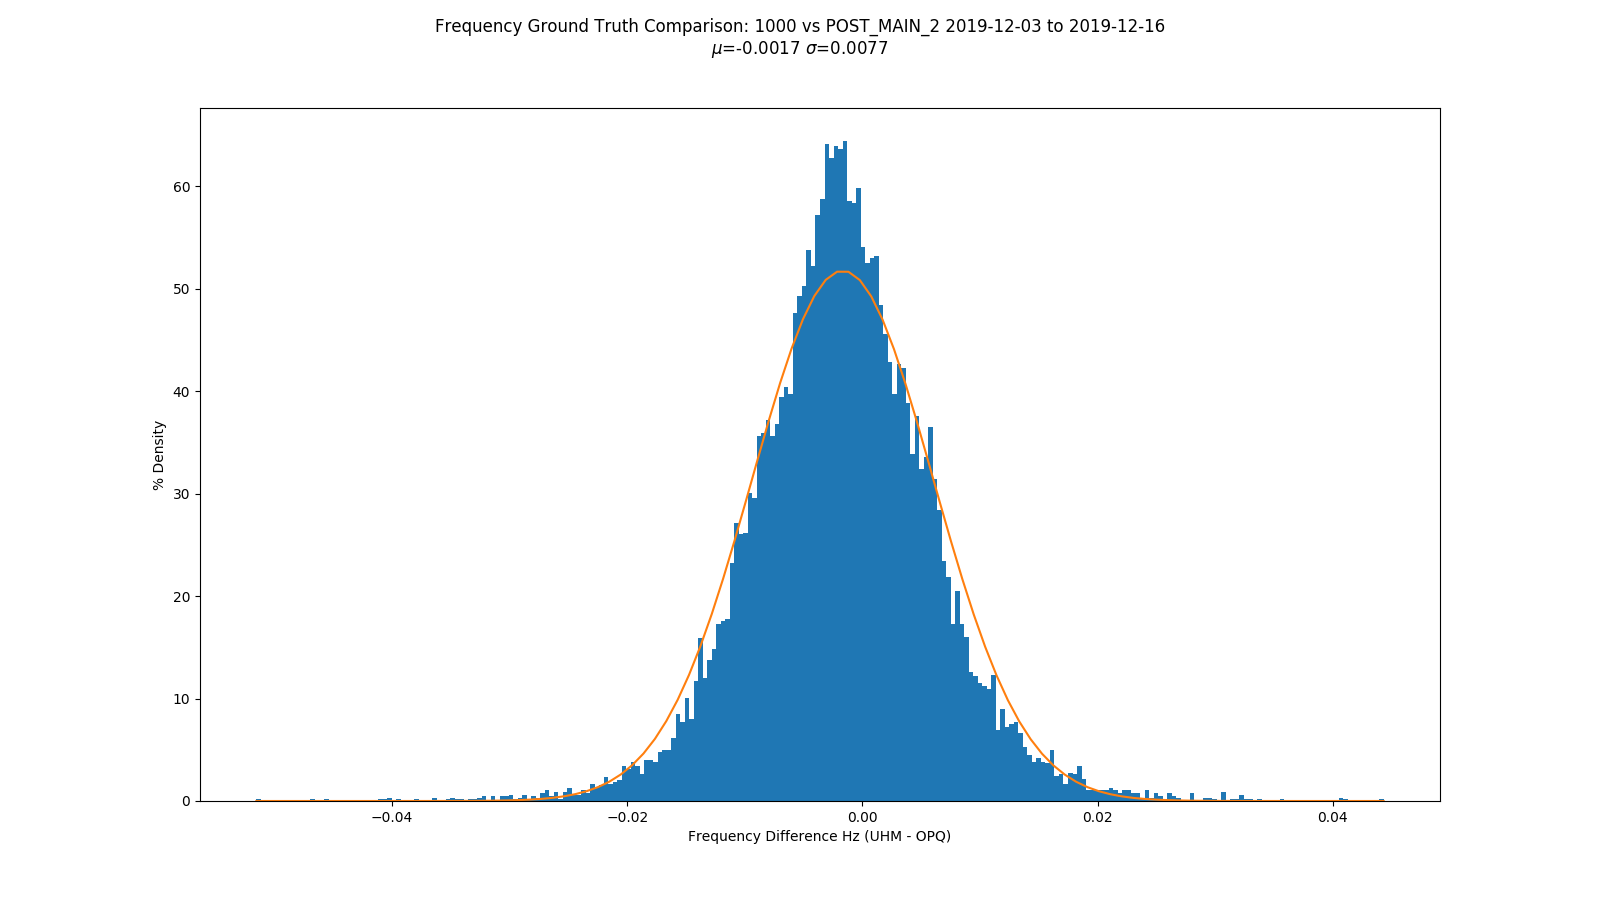
\includegraphics[width=0.75\linewidth]{figures/f_hist_1000_POST_MAIN_2.png}
    \caption{Frequency OPQ Box 1000 vs POST\_MAIN\_1}
    \label{fig:f_hist}
\end{figure}

The rest of the Frequency comparisons look very similar and the results are summarized in Table~\ref{table:gt_f}.

\begin{table}[H]
    \centering
    \caption{Frequency Trend Comparisons}
    \begin{tabularx}{\textwidth}{lXll}
        \toprule
        \textbf{OPQ Box} & \textbf{UHM Ground Truth Sensor} & \boldmath{$\mu$} & \boldmath{$\sigma$} \\
        \midrule
        1000 & POST\_MAIN\_1 & -0.0018 & 0.0079 \\
        1000 & POST\_MAIN\_2 & -0.0017 & 0.0079 \\
        1001 & HAMILTON..CH\_1 & -0.0007 & 0.0074 \\
        1001 & HAMILTON..CH\_2 & -0.0010 & 0.0074 \\
        1001 & HAMILTON..CH\_3 & -0.0012 & 0.0074 \\
        1001 & HAMILTON..MAIN\_1 & -0.0013 & 0.0074 \\
        1001 & HAMILTON..MAIN\_2 & -0.0011 & 0.0074 \\
        1001 & HAMILTON..MCC\_AC2 & -0.0009 & 0.0074 \\
        1002 & POST\_MAIN\_1 & -0.0018 & 0.0069 \\
        1002 & POST\_MAIN\_2 & -0.0017 & 0.0069 \\
        1003 & KELLER\_HALL\_MAIN & -0.0006 & 0.0073 \\
        1021 & MARINE\_SCIENCE\_MAIN\_A & -0.0010 & 0.0081 \\
        1021 & MARINE\_SCIENCE\_MAIN\_B & -0.0006 & 0.0081 \\
        1021 & MARINE\_SCIENCE\_MCC & 0.0003 & 0.0081 \\
        1022 & AG\_ENGINEERING\_MAIN & -0.0020 & 0.0078 \\
        1022 & AG\_ENGINEERING\_MCC & -0.0018 & 0.0078 \\
        1023 & LAW\_LIB\_MAIN & -0.0005 & 0.0078 \\
        1025 & KENNEDY\_THEATRE\_MAIN & -0.0013 & 0.0087 \\
        \bottomrule
    \end{tabularx}
    \label{table:gt_f}
\end{table}

As can be observed, the OPQ Boxes that we have co-located with UHM ground sensors track the Frequency quite accurately. In general we rarely see differences outside of 0.02 Hz and most sensors show a mean difference on the order of a mHz. These results are expected as grid stability relies heavily on the Frequency. Further, Frequency is generally affected at global scales rather than local scales, so we expect all UHM meters and OPQ Boxes to observe similar Frequency trends across the UHM micro-grid.

\subsubsection{Voltage Ground Truth Analysis}

OPQ Boxes measure RMS Voltage as a combination of three Voltage phases at 120 Volts. UHM ground truth meters measure RMS Voltage for each individual phase at different Voltages (480, 240, and 270). Because of these differences, the Voltages can not be compared directly and can only be performed for a small subset of our Boxes due to available ground truth data (those that contain Voltage channels for ``AB", ``BC", and ``CA").

In order to compare OPQ Box Voltages against UHM Voltages, a combination of Voltage values must exist within the ground truth data for each sensor with the following configurations: Voltage from phase A to phase B, Voltage from phase B to phase C, and Voltage from phase C to phase A. If these metrics exist, then the RMS value for the ground truth can be found by Equation~\ref{eq:gt_vrms} as described by Horowitz\cite{Horowitz:2015:AE:2960712} where $V_{AB}$, $V_{BC}$, and $V_{CA}$ provide the inter-phase Voltages reported by the UHM meters and $C$ is a constant dependent on the transformer configuration and the final step down Voltage. $C$ was empirically found to be 3.9985 for our data sets.

\begin{equation}
    V_{RMS} = \frac{1}{\sqrt{3}C} \sqrt{V_{AB}^2 + V_{BC}^2 + V_{CA}^2}
    \label{eq:gt_vrms}
\end{equation}

As an example, Figure~\ref{fig:v_hist} provides the difference in $V_{RMS}$ between OPQ Box 1000 and the UHM POST\_MAIN\_1 meter.

\begin{figure}[H]
    \centering
    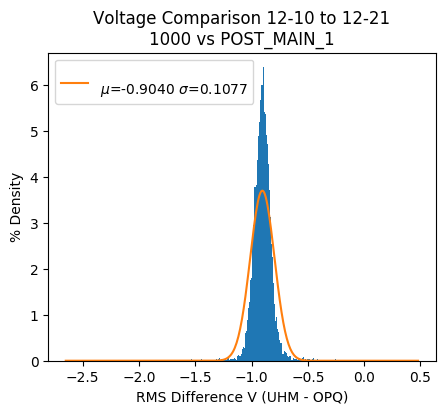
\includegraphics[width=0.75\linewidth]{figures/v_hist_1000_POST_MAIN_1.png}
    \caption{Voltage OPQ Box 1000 vs POST\_MAIN\_1}
    \label{fig:v_hist}
\end{figure}

Box 1000 averages about .9V higher than what is observed at the ground truth meter.

Some of the difference comparisons display multiple distributions which might be explained by the cycling of Voltage conditioning equipment and by larger loads on the grid during day time hours. However, I do not have enough information about the UH micro-grid detailed operations to be completely certain about these claims.

For example, Figure~\ref{fig:v_hist_ii} compares Box 1001 in POST to the POST\_MAIN\_1 meter.

\begin{figure}[H]
    \centering
    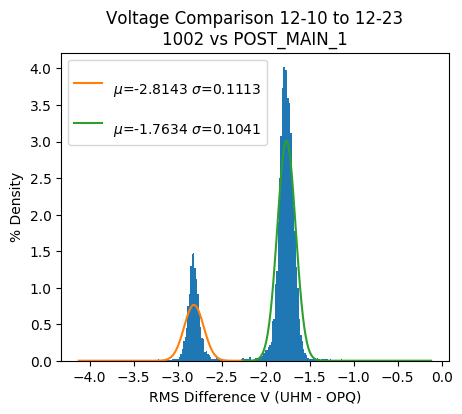
\includegraphics[width=0.75\linewidth]{figures/v_hist_1002_POST_MAIN_1.png}
    \caption{Voltage OPQ Box 1002 vs POST\_MAIN\_1}
    \label{fig:v_hist_ii}
\end{figure}

The green Gaussian fit shows Voltages collected during night time hours where the orange Gaussian fit shows values collected during the day time hours. It's interesting that Box 1000 and Box 1002 show such different results even though the Boxes are located on the same floor within the same building. The Boxes are however opposite each other within the building. I suspect that these Boxes are serviced by different electrical mains within the building. These claims are further supported by THD ground truth analysis in the following section which contains THD data for each electrical main.

Even more interesting is that several of our Voltage comparisons show three separate Gaussian distributions. As example, Figure~\ref{fig:v_hist_iii} compares Voltage values between Box 1021 and the MARINE\_SCIENCE\_MAIN\_A\_MTR.

\begin{figure}[H]
    \centering
    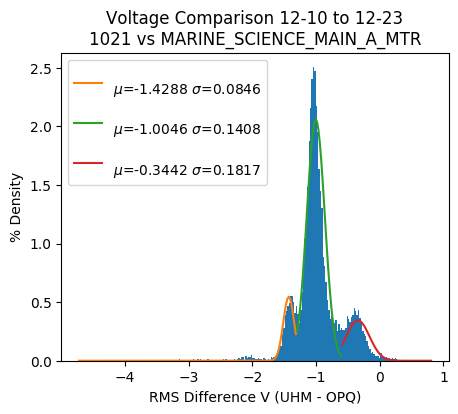
\includegraphics[width=0.75\linewidth]{figures/v_hist_1021_MARINE_SCIENCE_MAIN_A_MTR.png}
    \caption{Voltage OPQ Box 1021 vs MARINE\_SCIENCE\_MAIN\_A\_MTR}
    \label{fig:v_hist_iii}
\end{figure}

Here we can see that most of our values average about 1V higher than that of the ground truth with other peaks at 0.3V and 1.4V above the ground truth data.

Table~\ref{table:gt_v} summarizes the Voltage comparisons.

\begin{table}[H]
    \centering
    \caption{Voltage Trend Comparisons}
    \begin{tabularx}{\textwidth}{lXll}
        \toprule
        \textbf{OPQ Box} & \textbf{UHM Ground Truth Sensor} & \boldmath{$\mu$} & \boldmath{$\sigma$} \\
        \midrule
        1000 & POST\_MAIN\_1 & -0.9040 & 0.1077 \\
        1001 & HAMILTON..CH\_1 & -2.8192 -2.1797 -1.5725 & 0.2291 0.1516 0.2321 \\
        1001 & HAMILTON..CH\_2 & -3.0246 -2.3877 -1.7756 & 0.2310 0.1514 0.2285 \\
        1001 & HAMILTON..CH\_3 & -2.6499 -2.0276 -1.4360 & 0.2426 0.1419 0.2255 \\
        1001 & HAMILTON..MAIN\_1 & -2.5372 -1.9135 -1.3196 & 0.2346 0.1396 0.2361 \\
        1001 & HAMILTON..MAIN\_2 & -2.3670 -1.7215 -1.1026 & 0.2392 0.1519 0.2132 \\
        1001 & HAMILTON..MCC\_AC1 & -2.7611 -2.0735 -1.4276 & 0.2242 0.1886 0.2092 \\
        1001 & HAMILTON..MCC\_AC2 & -2.6994 -2.0377 -1.4231 & 0.2413 0.1674 0.2115 \\
        1002 & POST\_MAIN\_1 & -2.8143 -1.7634 & 0.1113 0.1041 \\
        1021 & MARINE\_SCIENCE\_MAIN\_A & -1.4293 -1.0043 -0.3454 & 0.0849 0.1406 0.1802 \\
        1021 & MARINE\_SCIENCE\_MAIN\_B & 0.9882 1.4071 2.0456 & 0.0720 0.1312 0.2049 \\
        1021 & MARINE\_SCIENCE\_MCC & -1.6304 -1.2121 -0.5738 & 0.0887 0.1300 0.1894 \\
        1022 & AG\_ENGINEERING\_MAIN & 0.0947 & 0.1704 \\
        1022 & AG\_ENGINEERING\_MCC & 0.0482 & 0.1703 \\
        1023 & LAW\_LIB\_MAIN & 0.6286 & 0.1841 \\
        \bottomrule
    \end{tabularx}
    \label{table:gt_v}
\end{table}

The POST (1000), MSB, Ag. Engineering, and Law Library buildings provide the most accurate comparisons to ground truth with average differences between .5V and 1V.

Hamilton Library is a major outlier in that the ground truth comparisons are generally off by around 1.5 to 2.5 Volts. Hamilton Library is fed by three electrical mains each with multiple channels. Ground truth data is only collected on Hamilton Ph III. I suspect that our Box in Hamilton is serviced by one of the other phases. This claim is further supported by the THD comparison in the next section.

\subsubsection{THD Ground Truth Analysis}

Total Harmonic Distortion (THD) is collected by both OPQ Boxes and UHM ground truth sensors. The feature that was used to make THD comparisons is the AVERAGE\_VOLTAGE\_THD from the ground truth data. Similar to the Frequency comparison, I subtracted the OPQ THD observations from the UHM THD observations and created histograms of the differences. I also attempted to fit the data with a Normal Distribution, but had less success than with the Frequency. This is due to the fact that several of the distribution do not follow a Gaussian, but instead present two separate Gaussian distributions.

The multiple distributions appear to be related to time of day and point towards either power conditioning equipment cycling on and off or an increased electrical load causing higher amounts of THD during the day (or perhaps both). When there are multiple THD distributions, the distribution throughout the night time hours is more accurate than the distribution created during day time hours.

Figure~\ref{fig:gt_thd_i} compares THD between the Pacific Ocean Science and Technology building (POST) OPQ Boxes and POST UHM sensors.

\begin{figure}[h]
    \begin{tabular}{cc}
        \subfloat[1000 vs. POST\_MAIN\_1]{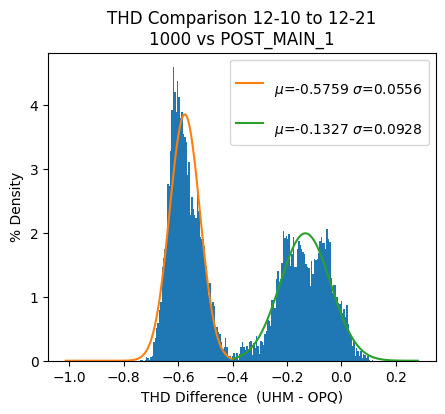
\includegraphics[width = 0.45\linewidth]{figures/thd_hist_1000_POST_MAIN_1.png}} &
        \subfloat[1000 vs. POST\_MAIN\_2]{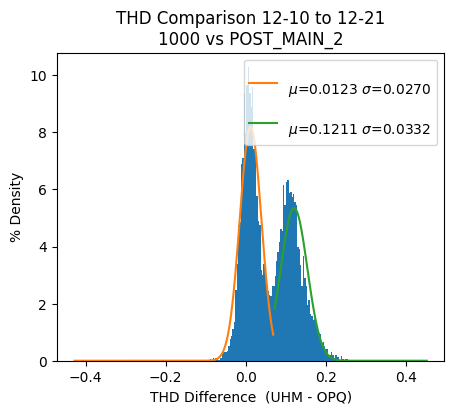
\includegraphics[width = 0.45\linewidth]{figures/thd_hist_1000_POST_MAIN_2.png}} \\
        \subfloat[1002 vs. POST\_MAIN\_1]{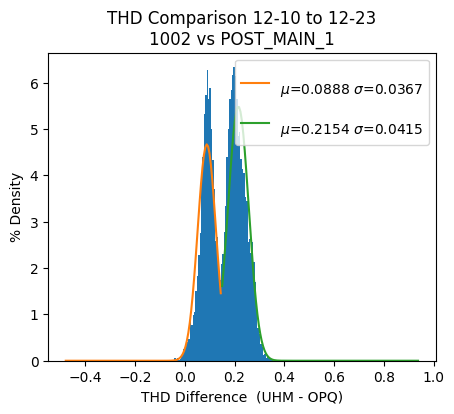
\includegraphics[width = 0.45\linewidth]{figures/thd_hist_1002_POST_MAIN_1.png}} &
        \subfloat[1002 vs. POST\_MAIN\_2]{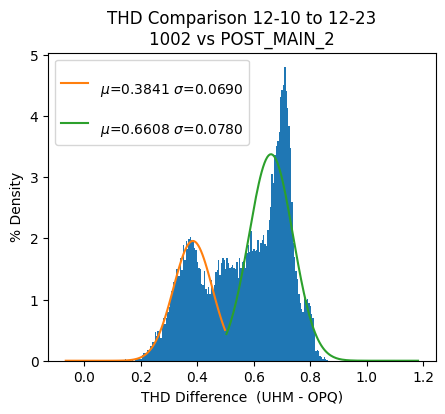
\includegraphics[width = 0.45\linewidth]{figures/thd_hist_1002_POST_MAIN_2.png}} \\
    \end{tabular}
    \caption{UHM THD vs. OPQ THD (POST)}
    \label{fig:gt_thd_i}
\end{figure}

The THD comparisons within the POST building provides several interesting features to discuss.

First, POST has two ground truth meters (POST\_MAIN\_1 and POST\_MAIN\_2) and two OPQ Boxes (1000 in the Collaborative Software Development Lab (CSDL) and 1002 in ICSpace). Both OPQ Boxes are on the third floor, roughly opposite each other in the building. As mentioned previously, I do not know exactly which electrical subsystem each OPQ Box is on when there are multiple electrical mains servicing a single building. In the case of POST, there are two electrical mains. I believe it's possible to guess which OPQ Box corresponds with which main by looking at the ground truth comparisons.

For instance, OPQ Box 1000 vs. POST\_MAIN\_2 provides a much smaller spread in THD difference (about .25\% THD) than OPQ Box 1000 vs. POST\_MAIN\_2 which has a spread of close to 1\% THD. I speculate that OPQ Box 1000 is on the same main as the POST\_MAIN\_2 meter. The opposite holds true for OPQ Box 1002. The spread for Box 1002 is smaller for POST\_MAIN\_1 (about 0.3\% THD) than it is for POST\_MAIN\_2 (about 0.6\% THD) which leads me to speculate that Box 1002 may be serviced by the same electrical main as the POST\_MAIN\_1 meter. These assumptions fit with assumptions made about the Voltage comparisons in the previous sections providing credence to the idea that 1000 and 1002 are serviced by separate mains with POST.

Table~\ref{table:gt_thd} summarizes the best Gaussian fit for THD comparisons between OPQ Boxes and available ground truth data.

\begin{table}[h]
    \centering
    \caption{THD Trend Comparisons}
    \begin{tabularx}{\textwidth}{lXll}
        \toprule
        \textbf{OPQ Box} & \textbf{UHM Ground Truth Sensor} & \boldmath{$\mu$} & \boldmath{$\sigma$} \\
        \midrule
        1000 & POST\_MAIN\_1 & -0.5759 -0.1327 & 0.0556 0.0928 \\
        1000 & POST\_MAIN\_2 & 0.0123 0.1200 & 0.0270 0.0320 \\
        1001 & HAMILTON..CH\_1 & 1.4245 & 0.4121 \\
        1001 & HAMILTON..CH\_2 & 1.4327 & 0.4114 \\
        1001 & HAMILTON..CH\_3 & 1.3943 & 0.4153 \\
        1001 & HAMILTON..MAIN\_1 & 1.4314 & 0.4072 \\
        1001 & HAMILTON..MAIN\_2 & 0.9872 1.6370 & 0.1339 0.3078 \\
        1001 & HAMILTON..MCC\_AC1 & 1.4338 & 0.4132 \\
        1001 & HAMILTON..MCC\_AC2 & 1.4441 & 0.4133 \\
        1002 & POST\_MAIN\_1 & 0.0888 0.2154 & 0.0367 0.0415 \\
        1002 & POST\_MAIN\_2 & 0.3875 0.6652 & 0.0655 0.0796 \\
        1021 & MARINE\_SCIENCE\_MAIN\_A & -0.6964 & 0.1156 \\
        1021 & MARINE\_SCIENCE\_MAIN\_B & 0.3098 0.5649 & 0.0725 0.0601 \\
        1021 & MARINE\_SCIENCE\_MCC & -0.6938 & 0.1160 \\
        1022 & AG\_ENGINEERING\_MAIN & 0.5406 & 0.0421 \\
        1022 & AG\_ENGINEERING\_MCC & 0.4993 & 0.0433 \\
        \bottomrule
    \end{tabularx}
    \label{table:gt_thd}
\end{table}

All comparisons (except for those at Hamilton Library) show average differences of around .5\% THD. Similar to what was discussed in the previous section comparing Voltage values, Hamilton remains the single outlier in our data set. Here, I observed upwards of 1.5\% THD difference across Hamilton based meters. This continues to lead me to believe that the OPQ Box in Hamilton is serviced by a different main that that of the HAMILTON\_PH\_III ground truth meters.

To summarize the comparison of OPQ Measurements and Trends to ground truth data, I showed that co-located OPQ Boxes and UHM ground truth meters trend quite closely together (except for at Hamilton Library) for low level metrics. Frequency is the most accurate metric, followed by THD and Voltage. I would have liked to have seen smaller differences and tighter bounds on the Voltage and THD comparisons, but differences of .5\% THD and .5V are still acceptable. I also wish I had a more concrete explanation for the multiple Gaussian distributions present in the THD and Voltage comparisons.

\subsubsection{Mauka Event Ground Truth Analysis}

Events contain metadata and a window of raw data that may or may not contain signals of interest. Events are produced in OPQ by two components. Mauka's threshold based Event detector and Napali's statistical based Event detector. This section focuses on Mauka's threshold based Event detection methods as the Napali Event Trigger is the focus of another Ph.D. dissertation in our research group.

Events generated by Mauka do not store information about which metric was used to generate that Event (Frequency, Voltage, or THD). When Mauka's Event detector was implemented, this seemed reasonable as Events are not supposed to make any type of assumption about what is non-nominal about the data, only that something non-nominal was observed.

Future implementations of the Mauka Event detector should store extra metadata about which metric was used to create an Event. This metric would be useful when comparing Events generated by Mauka to ground truth data using thresholding analysis.

In order to compare Mauka Events to ground truth data, I applied similar thresholds to those used by Mauka's Event detector to the ground truth data. The thresholds that were applied are $\pm$.16\% nominal Frequency, $\pm$2.5\% nominal Voltage, and +3\% THD. I then normalized the ground truth data by centering each feature's thresholds at zero and then counted the number of zero crossings for each feature and threshold for that feature.

Because the ground truth data is averaged over a minute window, I bin all Events by minute windows as well and only count windows that contain Events. I then compared the number of Events found by thresholding the ground truth data to the binned Events observed by Mauka. The results are shown in Table~\ref{table:gt_events}.

\begin{table}[h]
    \centering
    \caption{Events Comparisons}
    \begin{tabularx}{\textwidth}{lXll}
        \toprule
        \textbf{OPQ Box} & \textbf{UHM Ground Truth Sensor} & \textbf{OPQ Events} & \textbf{Ground Truth Events} \\
        \midrule
        1000 & POST\_MAIN\_1 & 580 & 928 \\
        1001 & HAMILTON\_LIB..CH\_1 & 291 & 394 \\
        1001 & HAMILTON\_LIB..CH\_2 & 291 & 380 \\
        1001 & HAMILTON\_LIB..CH\_3 & 291 & 371 \\
        1001 & HAMILTON\_LIB..MAIN\_1 & 291 & 375 \\
        1001 & HAMILTON\_LIB..MAIN\_2 & 291 & 615 \\
        1001 & HAMILTON\_LIB..MCC\_AC2 & 291 & 375 \\
        1002 & POST\_MAIN\_1 & 2678 & 928 \\
        1021 & MARINE\_SCIENCE\_MAIN\_A & 3613 & 379 \\
        1021 & MARINE\_SCIENCE\_MAIN\_B & 3613 & 821 \\
        1021 & MARINE\_SCIENCE\_MCC & 3613 & 391 \\
        1022 & AG\_ENGINEERING\_MAIN & 1605 & 929 \\
        1022 & AG\_ENGINEERING\_MCC & 1605 & 1138 \\
        \bottomrule
    \end{tabularx}
    \label{table:gt_events}
\end{table}

To perform this comparison, I required all three major features used by Mauka's Event generator, Frequency (``Frequency"), Voltage (``VAB", ``VBC", and ``VCA"), and THD (AVERAGE\_VOLTAGE\_THD). Ground truth data with all required features only provides co-located UHM sensors for OPQ Boxes 1000, 1001, 1002, 1021, and 1022.

Boxes 1000, 1001, and 1022 provide the best comparisons to ground truth. Mauka observes about 63\% of the ground truth Events for Box 1000 and 78\% for Box 1001. Mauka observed about 30\% more Events for Box 1022 as compared to ground truth data.

Boxes 1002 and 1021 show fairly anomalous results compared to the ground truth.

One interesting thing that I gathered during this comparison is that the main force driving Event generation within Mauka is THD Events. THD thresholds were set at 3\% for Event generation. Most ground truth data shows that ~80\% of all Events generated are likely caused by crossing the THD thresholds with close to 18\% being caused by Voltage threshold crossings. Only a very small percentage of Events generated were generated by Frequency threshold crossings. This means that observed differences in THD and Voltage readings between OPQ Boxes and ground truth sensors explain the differences that can be observed between ground truth data and OPQ Boxes.

For example, let's examine Box 1021 as a case study which observed 3,613 Events while ground truth only observed 391 Events. Figure~\ref{fig:gt_all_msb} shows the ground truth data for the MARINE\_SCIENCE\_MCC\_MTR sensor.

\begin{figure}[H]
    \centering
    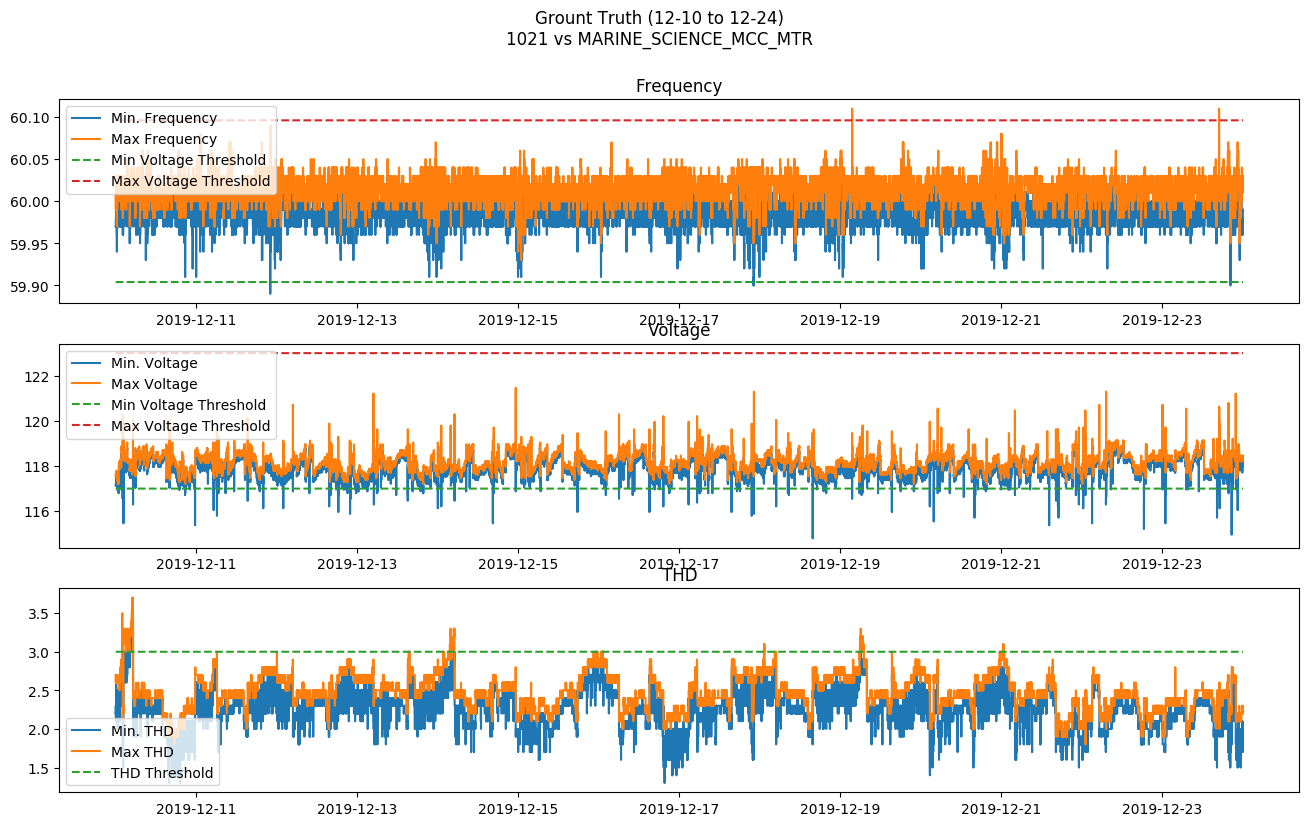
\includegraphics[width=\linewidth]{figures/gt_all_1021_MARINE_SCIENCE_MCC_MTR.png}
    \caption{Ground Truth MARINE\_SCIENCE\_MCC\_MTR}
    \label{fig:gt_all_msb}
\end{figure}

From the previous section, we saw Box 1021 observed THD that averages 0.7\% higher than what the ground truth observed. Adding the .7\% THD difference to the ground truth shown above pushes the THD just over threshold and causes Box 1021 to produce many more Events than what was observed by ground truth initially. These results are provided in Figure~\ref{fig:gt_adj_msb}.

\begin{figure}[H]
    \centering
    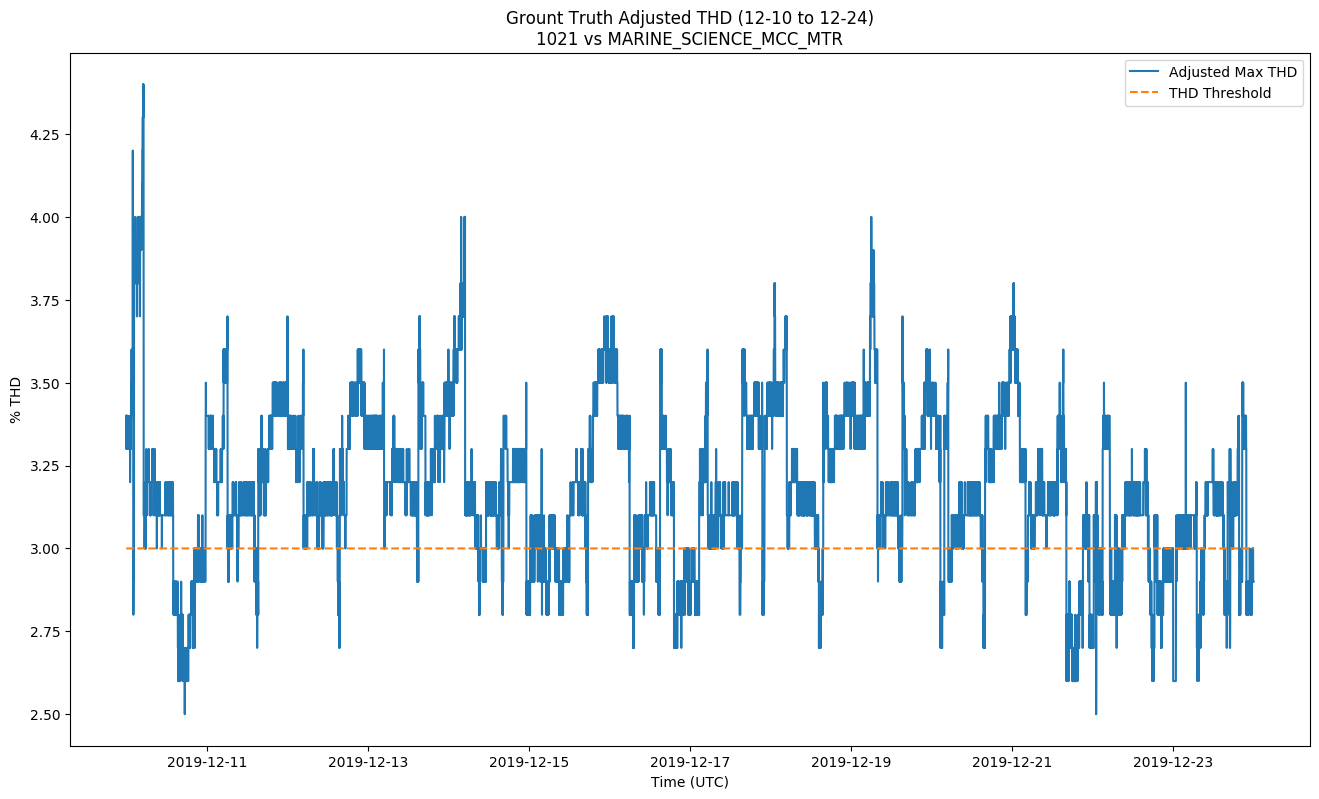
\includegraphics[width=\linewidth]{figures/gt_adj_1021_MARINE_SCIENCE_MCC_MTR.png}
    \caption{Ground Truth Adjusted THD MARINE\_SCIENCE\_MCC\_MTR}
    \label{fig:gt_adj_msb}
\end{figure}

Adding the average .7\% to the ground truth data increased the number of observed ground truth THD Events from 391 to 1252 bringing the total ground truth Events to 1562.

Perhaps the THD threshold is a bit too aggressive for Event generation and future work should look at relaxing this threshold a bit and observe how that affects the results.

The results for Box 1002 can also be explained using similar methodology. Figure~\ref{fig:gt_all_post_1} shows the ground truth readings at POST\_MAIN\_1.

\begin{figure}[H]
    \centering
    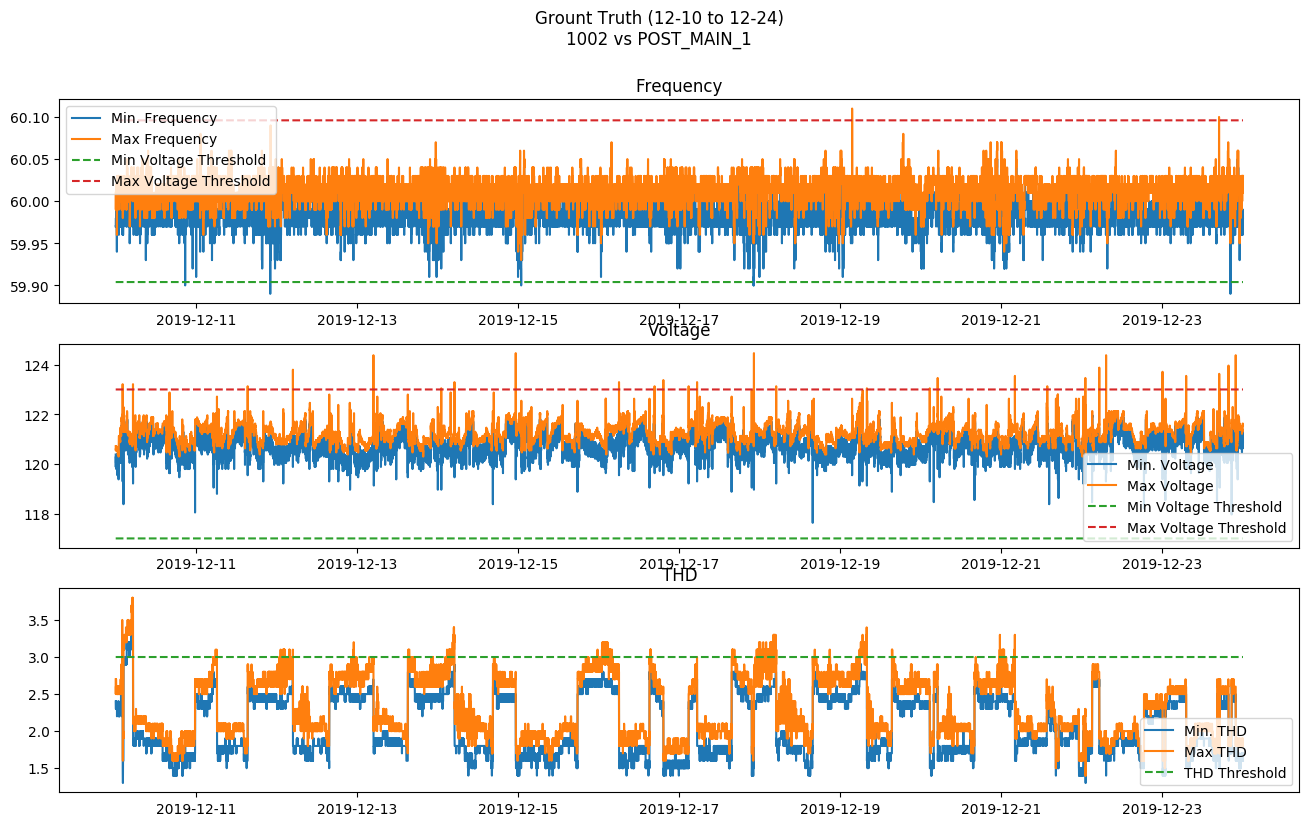
\includegraphics[width=\linewidth]{figures/gt_all_1002_POST_MAIN_1.png}
    \caption{Ground Truth POST\_MAIN\_1}
    \label{fig:gt_all_post_1}
\end{figure}

This time, THD is not the cause of the large difference in the comparison. Instead, it's the Voltage readings. Box 1002 reads on average 1.7 Volts higher than what is reported by ground truth. Figure~\ref{fig:gt_adj_post_1} shows the ground truth data adjusted to be 1.7 Volts higher.

\begin{figure}[H]
    \centering
    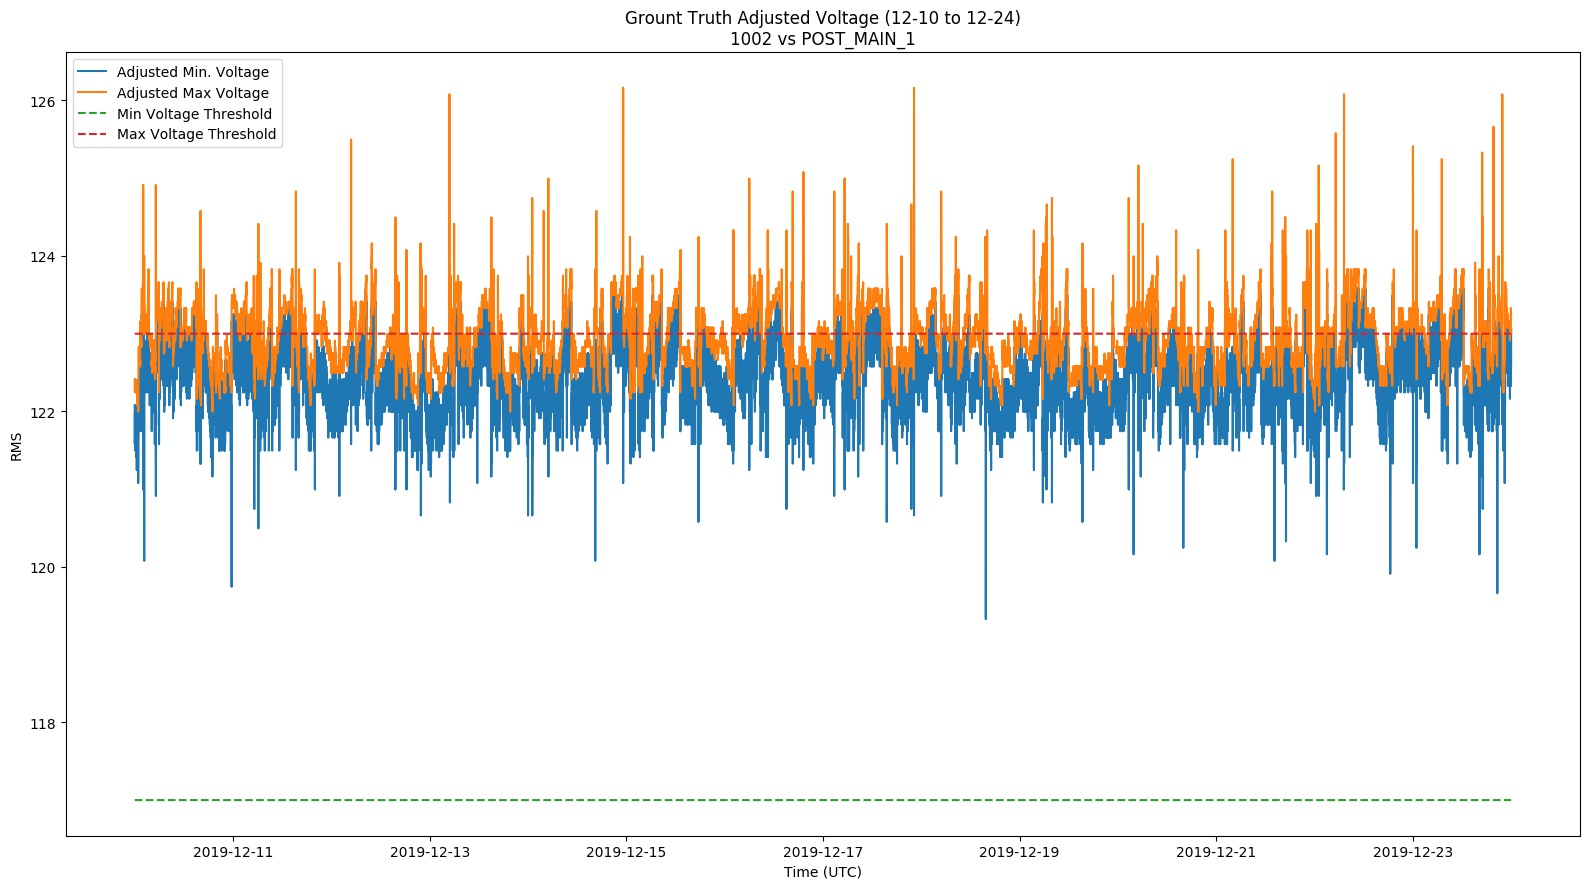
\includegraphics[width=\linewidth]{figures/gt_adj_1002_POST_MAIN_1.png}
    \caption{Ground Truth Voltage Adjusted POST\_MAIN\_1}
    \label{fig:gt_adj_post_1}
\end{figure}

Here, we can observe that the Voltage values are often passing the high Voltage threshold. This increases the number of Voltage Events from 34 to 1141 bringing the total observed ground truth Events to 2035 or 643 Events less than what OPQ Box 1002 observed.

What these results show is that the ground truth comparisons are largely affected by observed readings of THD and Voltage values by OPQ Boxes. These results also show that OPQ Boxes that produce large numbers of Events are caused by readings that hover near the feature thresholds that are utilized for Event creation.

The results from Event ground truth comparison are encouraging. The results show that although we may not be reading exactly what the ground truth sensors are reading, when adjusted for differences in low level metrics, expected Mauka Events match that of the ground truth data.

The next section will compare Mauka Incidents to ground truth data.

\subsubsection{Mauka Incident Ground Truth Analysis}

The OPQ ground truth data does not contain concepts that are related to Laha Incidents. In fact, the further we get away from the metrics that the ground truth provides (rolled-up one minute summaries), the harder it is to compare to higher levels in the Mauka hierarchy.

Instead, I apply thresholding to the ground truth data to determine where Incidents should have been observed verses when they were actually observed by Mauka. To complicate the matter, the OPQ ground truth data only provides features at a granularity of one minute. Therefore, I bin each individual Incident by minute and only count the number of bins that contain Incidents, similar to what was done for Events.

Using thresholding breaks down for many of the Incident types that rely on the duration of a disturbance to apply a classification (which is almost all of them). For instance, all IEEE defined PQ classifications rely on accurate durations of anomalous signals to apply a classification. This also holds true for Incidents that utilize industry standards such as ITIC or Semi-F47. These Incident types can not be compared to the ground truth data directly since ground truth data does not provide any notion of duration and only averages values over a one minute time window which is much too large for almost all of Mauka's Incident classifications. The best I can do for comparing Incidents is attempting to ensure that the threshold bounds make sense.

Incidents were compared using one month of data from December 1 to December 30.

\paragraph{Voltage Incidents Comparison}

Voltage Incidents include Voltage sags, swells and interruptions as well as Semi-F47 and ITIC classifications. All Voltage Incidents rely on the duration of the Incident in order to provide an accurate classification. Duration information is not provided by ground truth data. Instead, I use thresholding to determine where OPQ Incidents might have been observed. It's important to note here that Incidents observed by the ground truth data may not meet the duration thresholds to be classified by OPQ. I attempt to motivate this point using data from Events.

Table~\ref{table:gt_v_incidents} summarizes the results for the Voltage Incidents comparisons. Please note the abbreviations in the table where ``O." stands for an OPQ Box and ``U." stands for a UHM sensor.

\begin{table}[H]
    \centering
    \caption{Voltage Incidents Comparisons}
    \begin{tabularx}{\textwidth}{lXllll}
        \toprule
        \textbf{OPQ Box} & \textbf{UHM Ground Truth Sensor} & \textbf{O.Sags} & \textbf{O.Swells} & \textbf{U.Sags} & \textbf{U.Swells} \\
        \midrule
        1000 & POST\_MAIN\_1 & 0 & 0 & 2 & 108 \\
        1000 & POST\_MAIN\_2 & 0 & 0 & 2 & 346 \\
        1001 & HAMILTON\_LIB..CH\_1 & 34 & 0 & 90 & 8 \\
        1001 & HAMILTON\_LIB..CH\_2 & 34 & 0 & 104 & 2 \\
        1001 & HAMILTON\_LIB..CH\_3 & 34 & 0 & 82 & 10 \\
        1001 & HAMILTON\_LIB..MAIN\_1 & 34 & 0 & 80 & 12 \\
        1001 & HAMILTON\_LIB..MAIN\_2 & 34 & 0 & 38 & 18 \\
        1001 & HAMILTON\_LIB..MAIN\_AC1 & 34 & 0 & 90 & 12\\
        1001 & HAMILTON\_LIB..MAIN\_AC2 & 34 & 0 & 84 & 10\\
        1002 & POST\_MAIN\_1 & 2 & 0 & 2 & 108 \\
        1002 & POST\_MAIN\_2 & 2 & 0 & 2 & 346 \\
        1021 & MARINE\_SCIENCE\_MAIN\_A & 8 & 0 & 296 & 0 \\
        1021 & MARINE\_SCIENCE\_MAIN\_B & 8 & 0 & 2 & 62 \\
        1021 & MARINE\_SCIENCE\_MCC & 8 & 0 & 664 & 0 \\
        1022 & AG\_ENGINEERING\_MAIN & 8 & 0 & 48 & 10 \\
        1022 & AG\_ENGINEERING\_MCC & 8 & 0 & 52 & 10 \\
        1023 & LAW\_LIB\_MAIN & 0 & 0 & 30 & 10 \\
        \bottomrule
    \end{tabularx}
    \label{table:gt_v_incidents}
\end{table}

There are a couple of things to note here. Mauka did observe 8 Voltage swells over this time period all for Box 1008. However, we do not have ground truth data for this location and Mauka did not observe any other Voltage swells with co-located ground truth sensors.

All counts for OPQ are less than the counts shown by the OPQ ground truth data. This is important because the ground truth data does not provide any metric for swell or sag duration. This means that some percentage of the ground truth sags and swells durations are less than what is required to classify the data as an Incident by OPQ Mauka.

One of the reasons Mauka likely did not classify many Voltage swells is because they are much less common in general. Further, according to Power Standards Lab\cite{power_standards_lab_2017}, Voltage swells tend to be much smaller in duration compared to Voltage sags. This is due to the fact that Voltage swells are almost always caused by an abrupt decrease in load on the grid followed by rapid stabilization. Voltage sags on the other hand are caused by an increased load on the grid and last for as long as that load continues to persist. It's likely the Voltage spikes observed by the UHM sensors did not last long enough in duration to be classified as Mauka Incidents, however without more detailed ground truth data, this is only a hypothesis.

\paragraph{THD Incidents Comparison}

I compared THD observed by the UHM ground truth meters to THD observed by OPQ Boxes.

The OPQ Box computes THD over a window of six cycles. The window size that the UHM ground truth sensors utilize for THD calculations is unknown. Because the Mauka THD plugin computes THD per electrical cycle, I expect the THD generated by Mauka to be slightly higher than that of the OPQ Box Measurements or Trends which compute THD over a larger window.

This is caused by using a smaller THD computation window which has less of a chance to average out noise. On one hand, this provides THD per cycle which better exemplifies small transients in the data which would otherwise be averaged out using larger window lengths. On the other hand, measured THD will be higher due to added noise in the signal.

I empirically found that THD values calculated by Mauka add .5\% THD to the OPQ Box and UHM ground truth measurements. This added THD is due to added noise in the THD calculation caused by using a smaller window. Ground truth data had this constant added before comparing to THD Incidents produced by Mauka. Table ~\ref{table:gt_thd_incidents} summarizes the results of the THD Incidents comparison.

\begin{table}[H]
    \centering
    \caption{THD Incidents Comparisons}
    \begin{tabularx}{\textwidth}{lXllll}
        \toprule
        \textbf{OPQ Box} & \textbf{UHM Ground Truth Sensor} & \textbf{OPQ THD} & \textbf{UHM THD} \\
        \midrule
        1000 & POST\_MAIN\_1 & 3 & 0 \\
        1000 & POST\_MAIN\_2 & 3 & 0 \\
        1001 & HAMILTON\_LIB\_PH\_III\_CH\_1\_MTR & 41 & 456 \\
        1001 & HAMILTON\_LIB\_PH\_III\_CH\_2\_MTR & 41 & 464 \\
        1001 & HAMILTON\_LIB\_PH\_III\_CH\_3\_MTR & 41 & 281 \\
        1001 & HAMILTON\_LIB\_PH\_III\_MAIN\_1\_MTR & 41 & 491 \\
        1001 & HAMILTON\_LIB\_PH\_III\_MAIN\_2\_MTR & 41 & 465 \\
        1001 & HAMILTON\_LIB\_PH\_III\_MCC\_AC1\_MTR & 41 & 456 \\
        1001 & HAMILTON\_LIB\_PH\_III\_MCC\_AC2\_MTR & 41 & 443 \\
        1002 & POST\_MAIN\_1 & 3 & 0 \\
        1002 & POST\_MAIN\_2 & 3 & 0 \\
        1021 & MARINE\_SCIENCE\_MAIN\_A\_MTR & 59 & 0 \\
        1021 & MARINE\_SCIENCE\_MAIN\_B\_MTR & 59 & 481 \\
        1021 & MARINE\_SCIENCE\_MCC\_MTR & 59 & 0 \\
        1022 & AG\_ENGINEERING\_MAIN\_MTR & 21 & 111 \\
        1022 & AG\_ENGINEERING\_MCC\_MTR & 21 & 61 \\
        \bottomrule
    \end{tabularx}
    \label{table:gt_thd_incidents}
\end{table}

These results are not surprising. Similar to the Voltage Incidents, we observe that OPQ Boxes track less THD Incidents than the UHM ground truth meters. This is to be expected due to the fact that the Incidents are only classified when signals are non-nominal for specified durations. It's likely (yet unknown due to lack of detailed ground truth data) that the extraneous THD Incidents that were observed by the ground truth sensors did not meet the duration requirements for classification.

Boxes 1000 and 1002 provide the only surprising results in that the THD Incidents observed by Mauka were not observed by the UHM ground truth sensors. The Incidents correspond to high peaks in THD at those locations, but the peaks do not cross the THD threshold of 5\%. Since these Incidents correspond with peaks in the ground truth data, it is possible that the smaller THD computation window and added noise created these false positives.

\paragraph{Frequency Incidents Comparison}

Frequency Incidents are classified as either Frequency sags, swells, or interruptions.

Frequency is calculated by filtering a power signal and then fitting a sinusoid per cycle of that power signal. Because Frequency is calculated per cycle, I expect to see higher Frequency values than those compared to the OPQ Box. This is due to the fact that a smaller Frequency estimation window contains more noise. It is unknown what window the UHM sensors use for Frequency calculation, but since it trends so nicely with OPQ Box data, I suspect it is on the order of six cycles.

In order to compare Frequency Incidents with UHM ground truth data, the ground truth data must be scaled to account for the added noise provided by the smaller Frequency estimation windows. I empirically found the amount of added noise in the Frequency domain to be .21 Hz. This value was added to the maximum UHM values and subtracted from the minimum UHM values in order to provide an accurate comparison. The results are summarized in Table~\ref{table:gt_f_incidents}.

\begin{table}[H]
    \centering
    \caption{Frequency Incidents Comparisons}
    \begin{tabularx}{\textwidth}{lXllll}
        \toprule
        \textbf{OPQ Box} & \textbf{UHM Ground Truth Sensor} & \textbf{O.Sags} & \textbf{O.Swells} & \textbf{U.Sags} & \textbf{U.Swells} \\
        \midrule
        1000 & POST\_MAIN\_1 & 1004 & 926 & 4143 & 1813 \\
        1000 & POST\_MAIN\_2 & 1004 & 926 & 4039 & 1892 \\
        1001 & HAMILTON..CH\_1 & 341 & 186 & 3337 & 2091 \\
        1001 & HAMILTON..CH\_2 & 341 & 186 & 3526 & 1951 \\
        1001 & HAMILTON..CH\_3 & 341 & 186 & 3546 & 1896 \\
        1001 & HAMILTON..MAIN\_1 & 341 & 186 & 3876 & 2087 \\
        1001 & HAMILTON..MAIN\_2 & 341 & 186 & 3746 & 2123 \\
        1001 & HAMILTON..MCC\_AC1 & 341 & 186 & 3499 & 1988 \\
        1001 & HAMILTON..MCC\_AC2 & 341 & 186 & 3419 & 2055 \\
        1002 & POST\_MAIN\_1 & 297 & 522 & 4143 & 1813 \\
        1002 & POST\_MAIN\_2 & 297 & 522 & 4039 & 1892 \\
        1003 & KELLER\_HALL\_MAIN & 2680 & 2427 & 2549 & 1524 \\
        1021 & MARINE\_SCIENCE\_MAIN\_A & 3788 & 4269 & 3652 & 2134 \\
        1021 & MARINE\_SCIENCE\_MAIN\_B & 3788 & 4269 & 3455 & 2337 \\
        1021 & MARINE\_SCIENCE\_MCC & 3788 & 4269 & 3106 & 2678 \\
        1022 & AG\_ENGINEERING\_MAIN & 2218 & 2602 & 3435 & 1390 \\
        1022 & AG\_ENGINEERING\_MCC & 2218 & 2602 & 3380 & 1477 \\
        1023 & LAW\_LIB\_MAIN & 197 & 149 & 2437 & 1673 \\
        1025 & KENNEDY\_THEATRE\_MAIN & 1022 & 619 & 2823 & 1314 \\
        \bottomrule
    \end{tabularx}
    \label{table:gt_f_incidents}
\end{table}

Of all of the ground truth results, the Frequency comparison in the weakest. I suspect this is caused by the amount of noise inside the short Frequency estimation windows. For the most part, OPQ observed Frequency Incidents are less than possible UHM observed Incidents. This is expected since not all Frequency swells and sags will results in the creation of an Incident within Mauka. However, we see that Boxes 1003, 1021, and 1022 overestimate the amount of verified Frequency swells.

Future work on Frequency estimation should include experimenting with different sized windows in an attempt to remove some of the noise from the estimations.

\paragraph{Summarizing Ground Truth Comparisons}

Low level metrics for Frequency, Voltage, and THD were compared against metrics collected from OPQ ground truth sensors. The Frequency metrics provided the best fits, followed by Voltage and THD. Comparisons were made by subtracting the differences and finding the best Gaussian fits. Voltage and THD metrics sometimes exhibited multiple Gaussians.

Events were compared to UHM ground truth data by applying thresholding on the data and correcting for differences in low level metrics. Events were binned by minute to match ground truth bins. Mauka Events are accounted for and are slightly underrepresented if the ground truth data is to be believed.

Incidents were compared to UHM ground truth data by applying thresholding to the data and correcting for differences in noise generation. Voltage and THD Incidents are well characterized, but Frequency Incidents were not as accurate.

Other than Frequency Incidents, these results provide evidence that the OPQ Mauka system provides accurate measurements as compared to the ground truth. By the rule of transitivity, I would like to say that all other Incidents that rely on features not collected by the UHM ground truth sensors are hopefully well characterized by virtue of the fact that all of the data feeding into those Incidents are well characterized.

Future work should seek to find ground truth options that provide more details such as the duration of anomalies or something similar to Events so that Incidents can be more easily and more directly compared to the ground truth data.

\subsection{Ground Truth Analysis: Lokahi}\label{subsec:ground-truth-analysis:-lokahi}

The Lokahi Infrasound network is unique in that most Events and Incidents are generated manually over known signals of interest. That is, something happens and an Event and possible an Incident are generated from a known signal. All public Incidents identified by Lokahi framework have been sourced and vetted. Thus, the question of sensor accuracy is: how well does Lokahi characterize Infrasound signals using mobile devices? Results were found in accordance to the Evaluation section~\ref{subsec:validate-data-collected-by-lokahi-deployment}.

This topic was studied and discussed extensively in Asmar's dissertation ``Modernizing Infrasound Systems: Characterization and Analytics Approaches for Next-Generation Sensors"\cite{asmar19}.

In Asmar's dissertation, the author compared Infrasound signals obtained by mobile sensors to industry standard microphones (Bruel \& Kjaer Microphone Type 4193) and microbarometer sensors (MB3 digital microbarometer) for ground truth. The infrasound signals were generated by a calibrated rotary sub-woofer capable of accurately producing infrasound signals.

Figure~\ref{fig:asmar_1} shows the noise power spectral density levels between a mobile sensor with an iPrecision microphone and a B\&K ground truth sensor.

\begin{figure}[H]
    \centering
    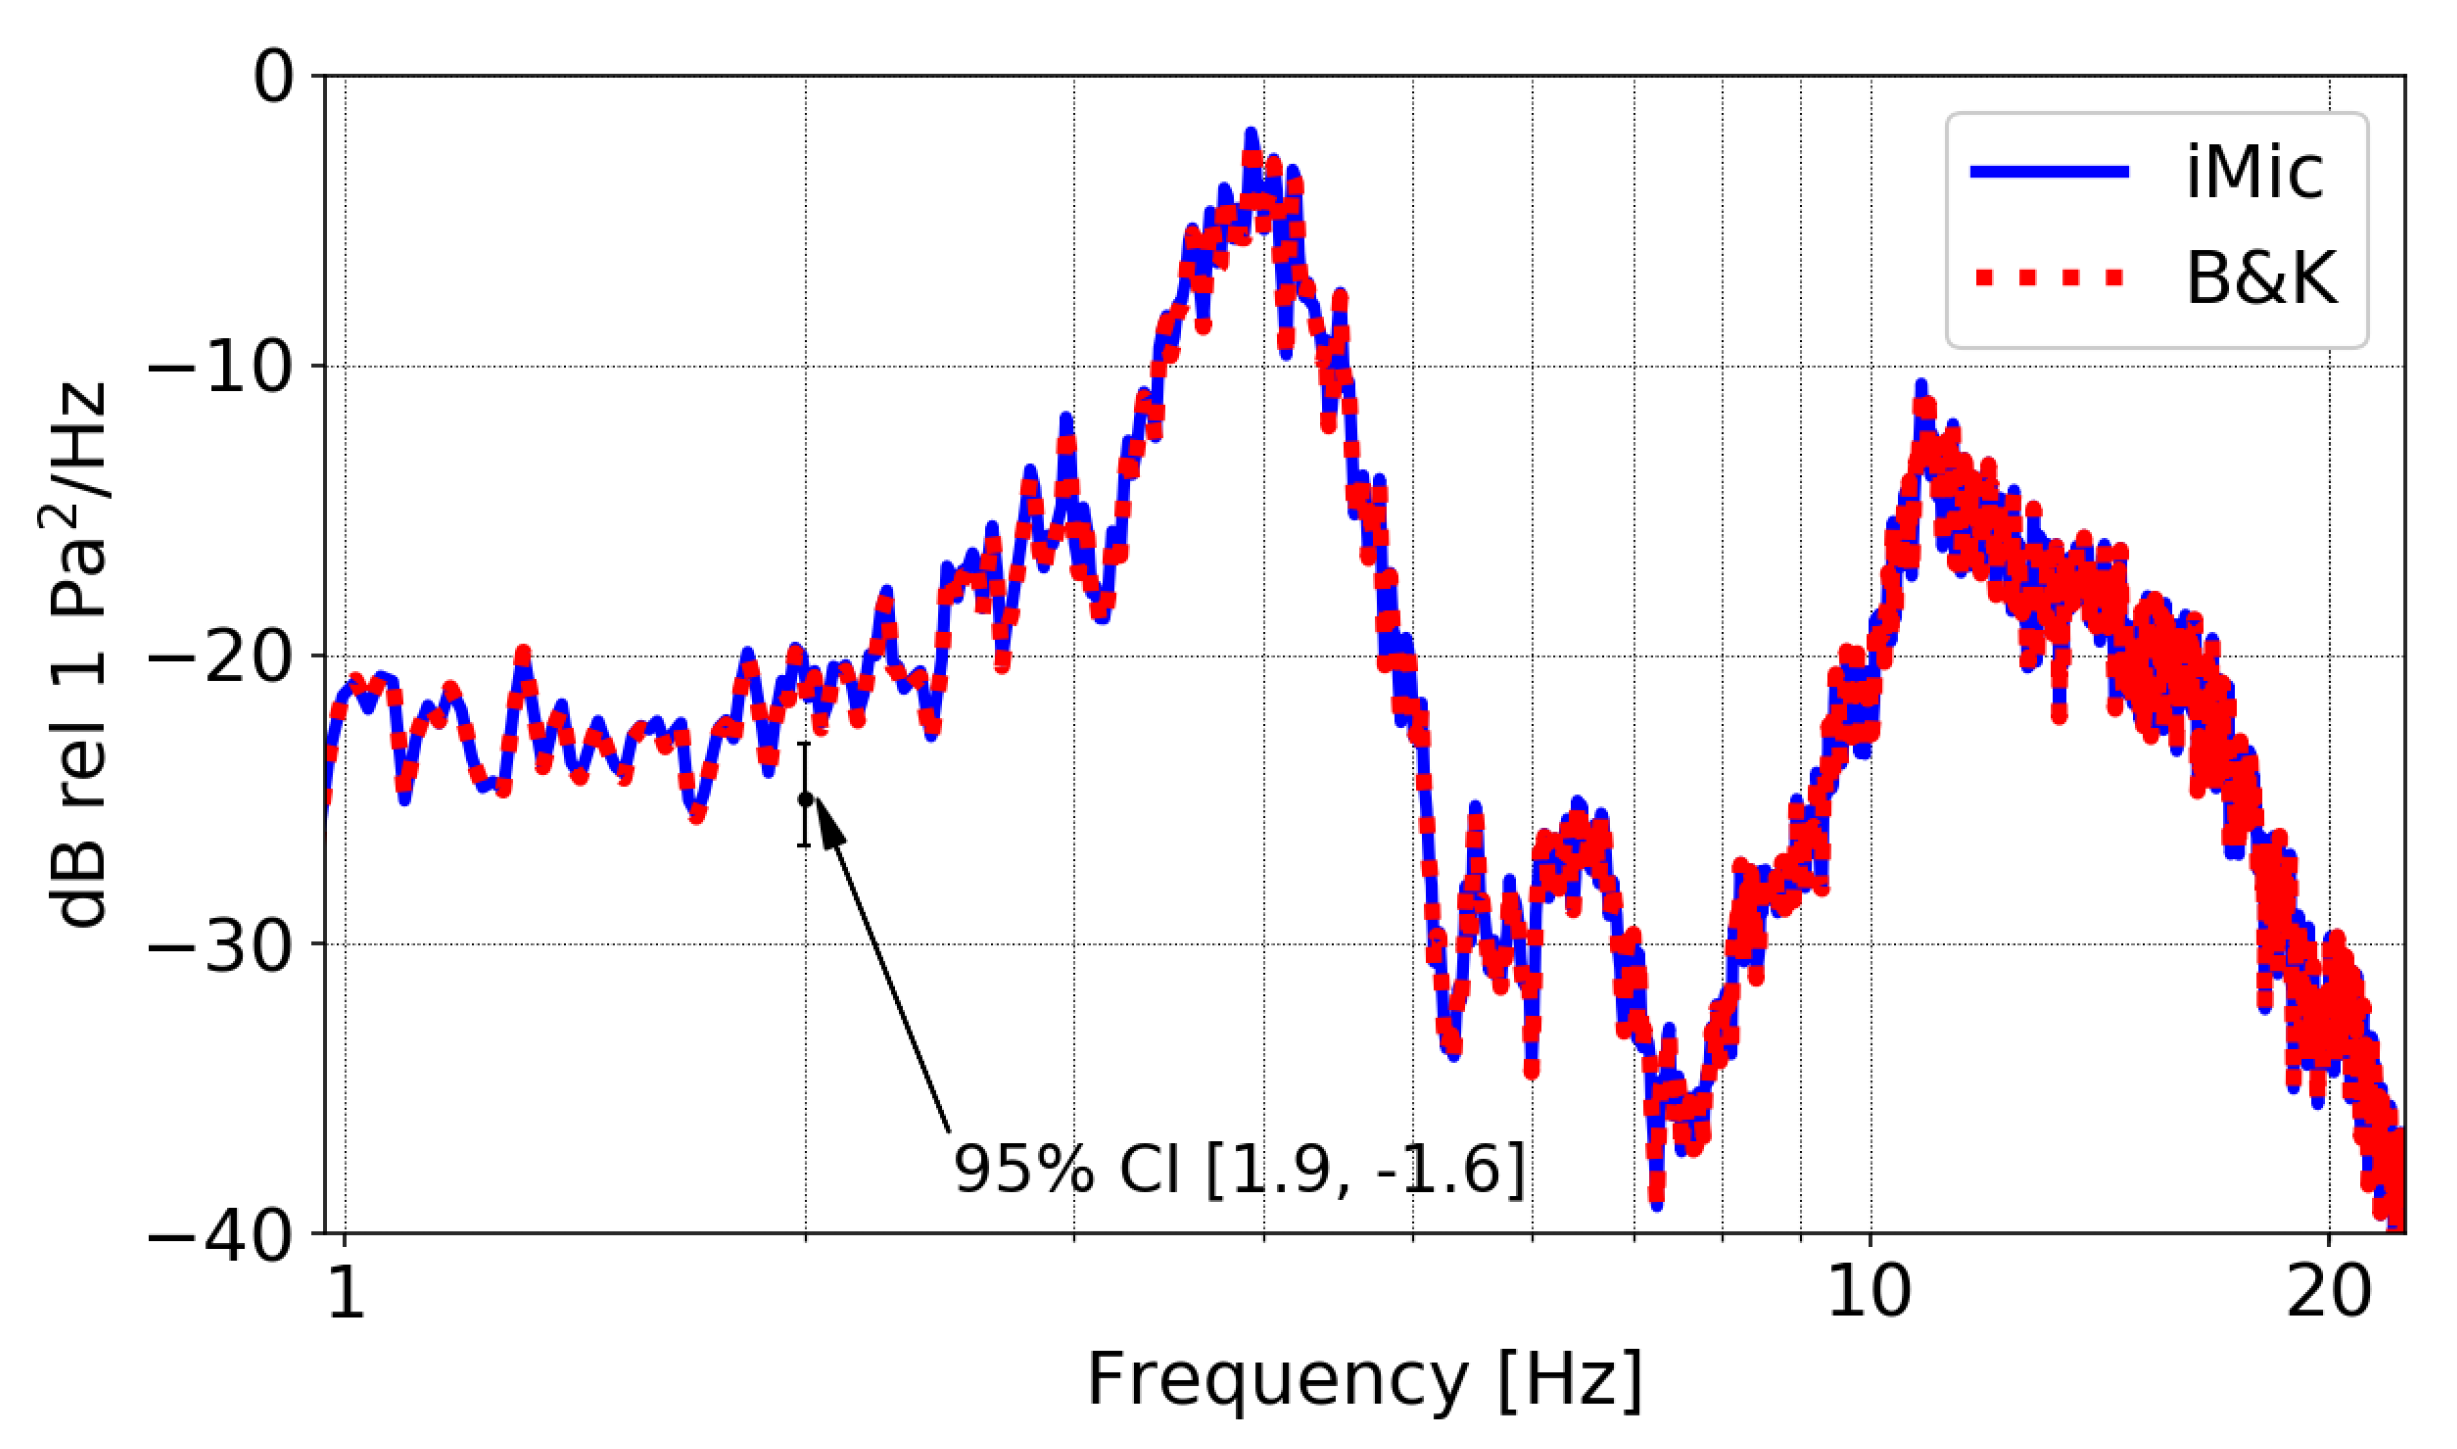
\includegraphics[width=\linewidth]{figures/asmar_1.png}
    \caption{Noise power spectral density levels with 95\% confidence interval (CI) [1.9, -1.6] dB re 1 $Pa^2$/Hz for iMic and B\&K across 0.97 to 22.4 Hz.}
    \label{fig:asmar_1}
\end{figure}

Figure~\ref{fig:asmar_2} shows the noise coherence results between a mobile sensor with an iPrecision microphone and a B\&K ground truth sensor.

\begin{figure}[H]
    \centering
    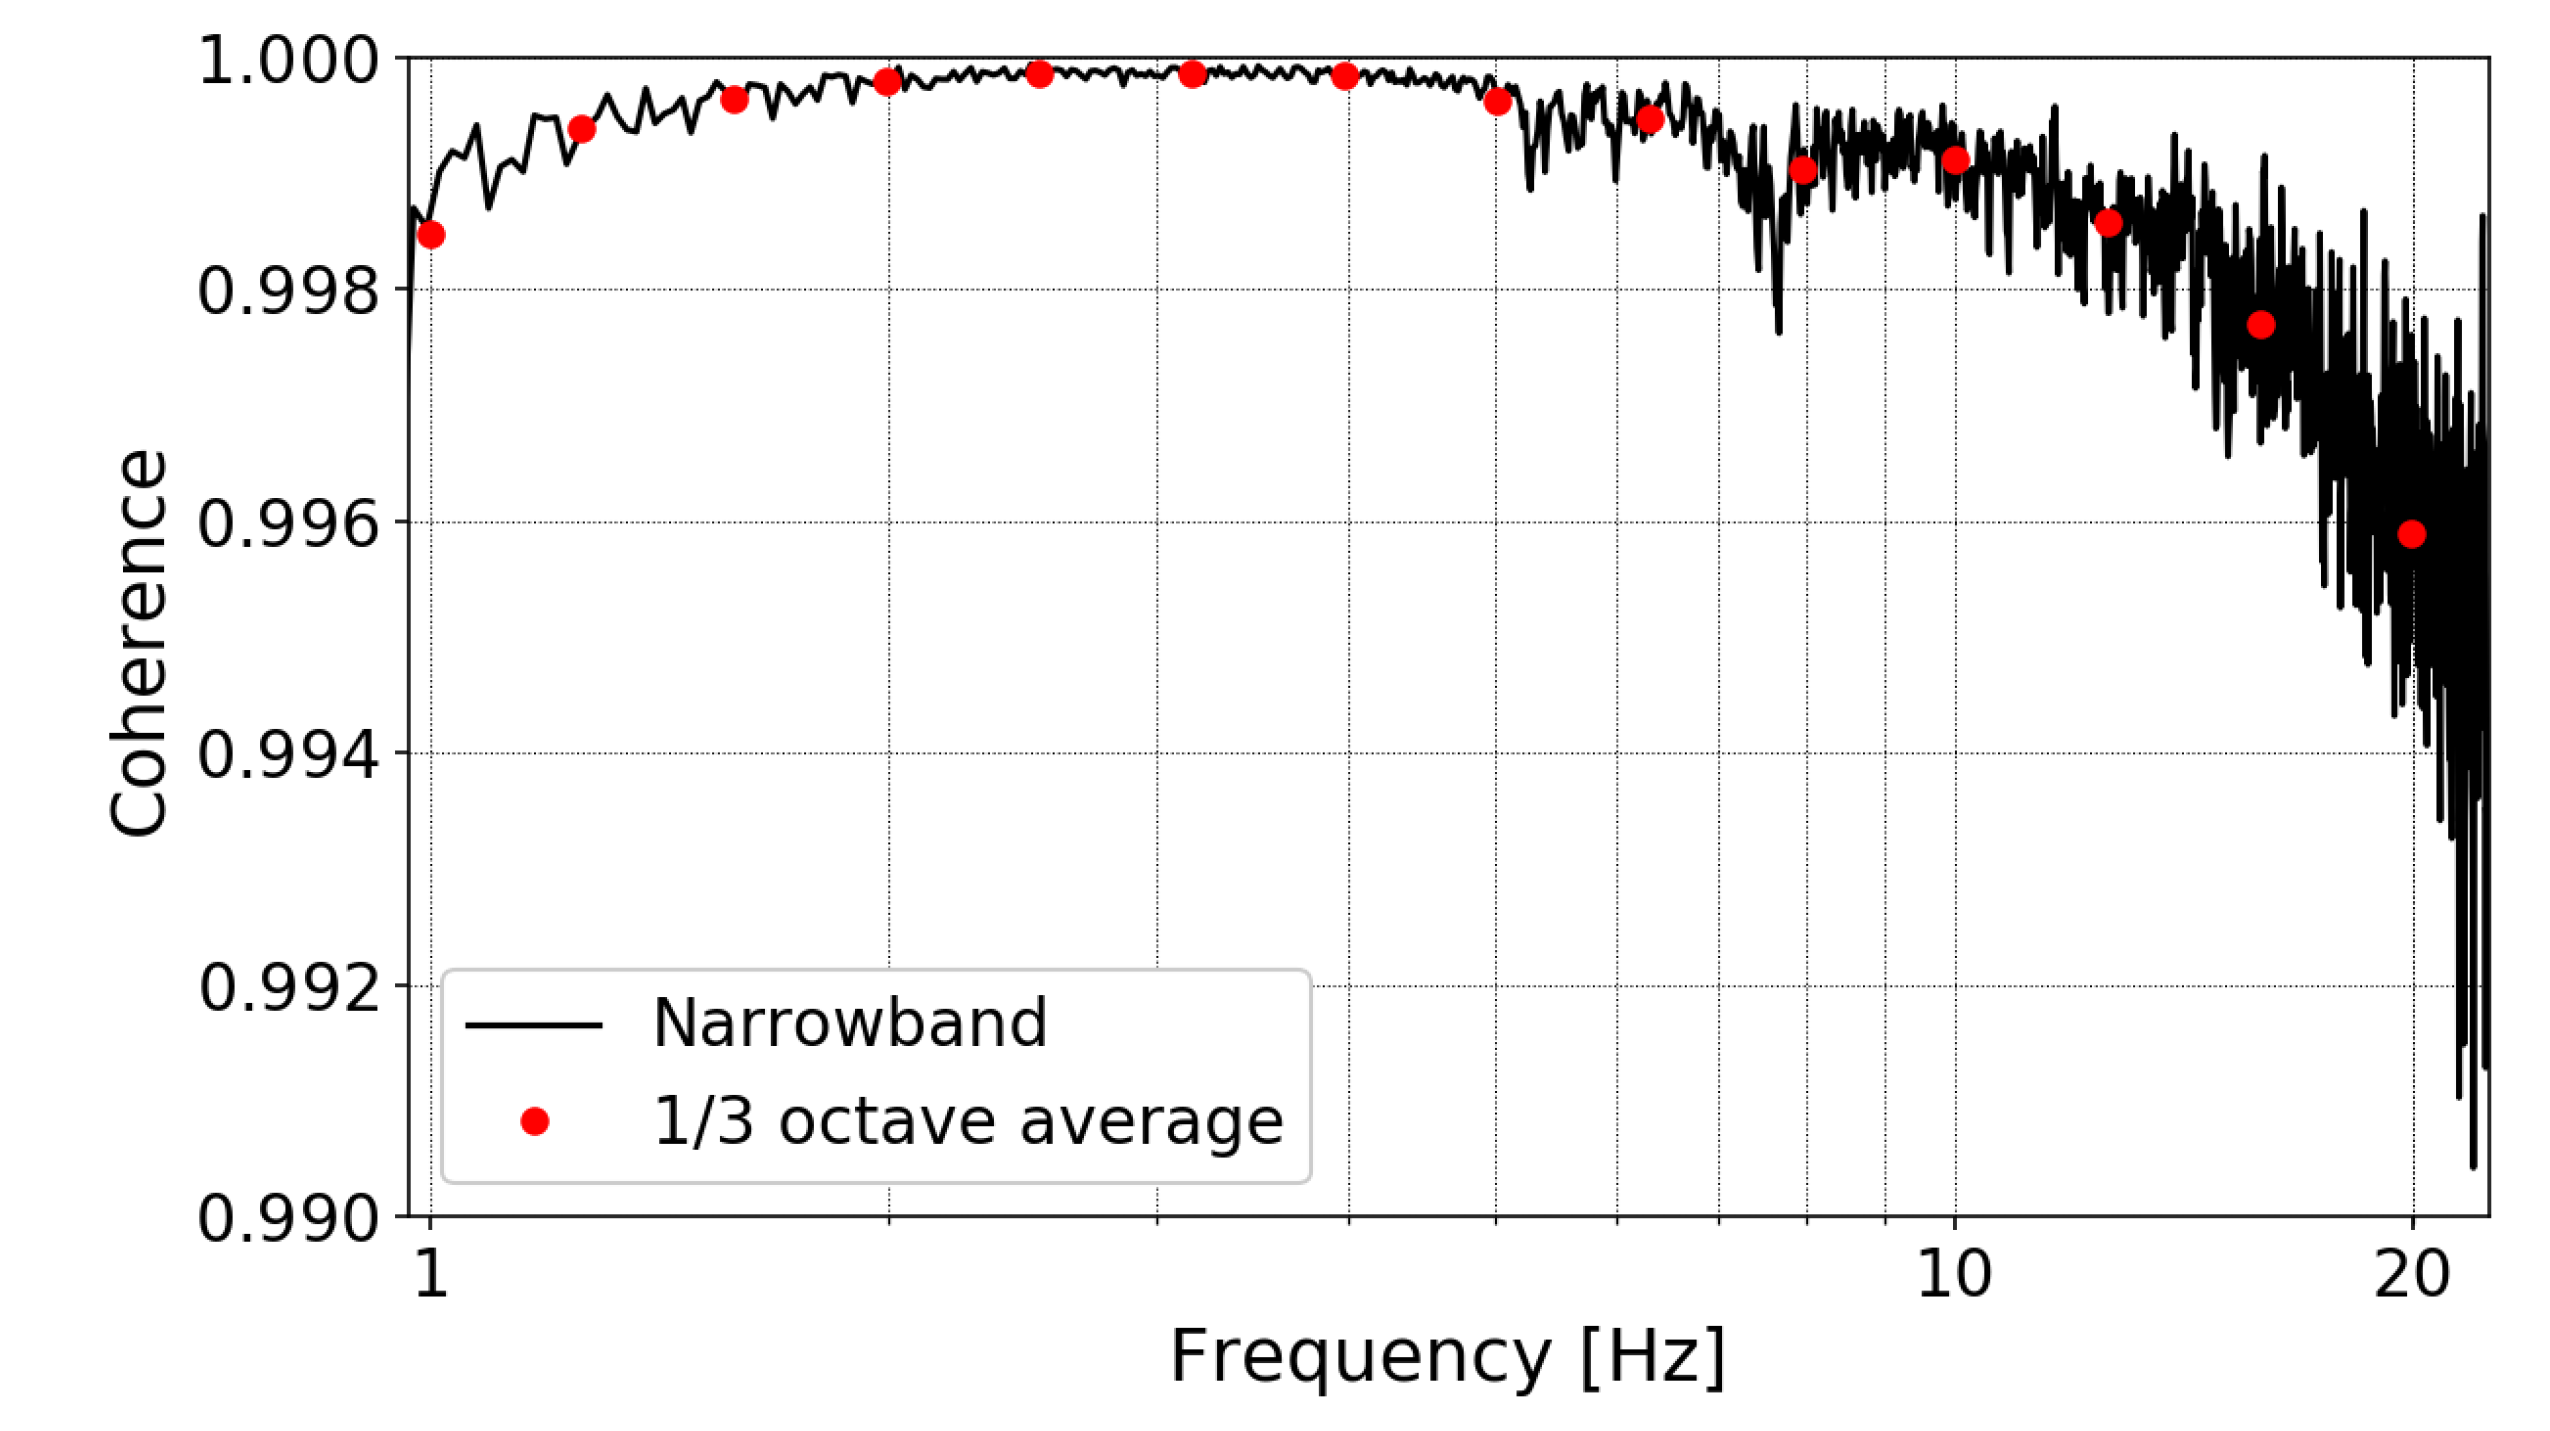
\includegraphics[width=\linewidth]{figures/asmar_2.png}
    \caption{Noise coherence results for iMic and B\&K across 0.97 to 22.4 Hz. The solid line represents the coherence between the sensors. The filled circles represent 1/3-octave band averaging.}
    \label{fig:asmar_2}
\end{figure}

Figure~\ref{fig:asmar_3} shows the noise response results between a mobile sensor with an iPrecision microphone and a B\&K ground truth sensor.

\begin{figure}[H]
    \centering
    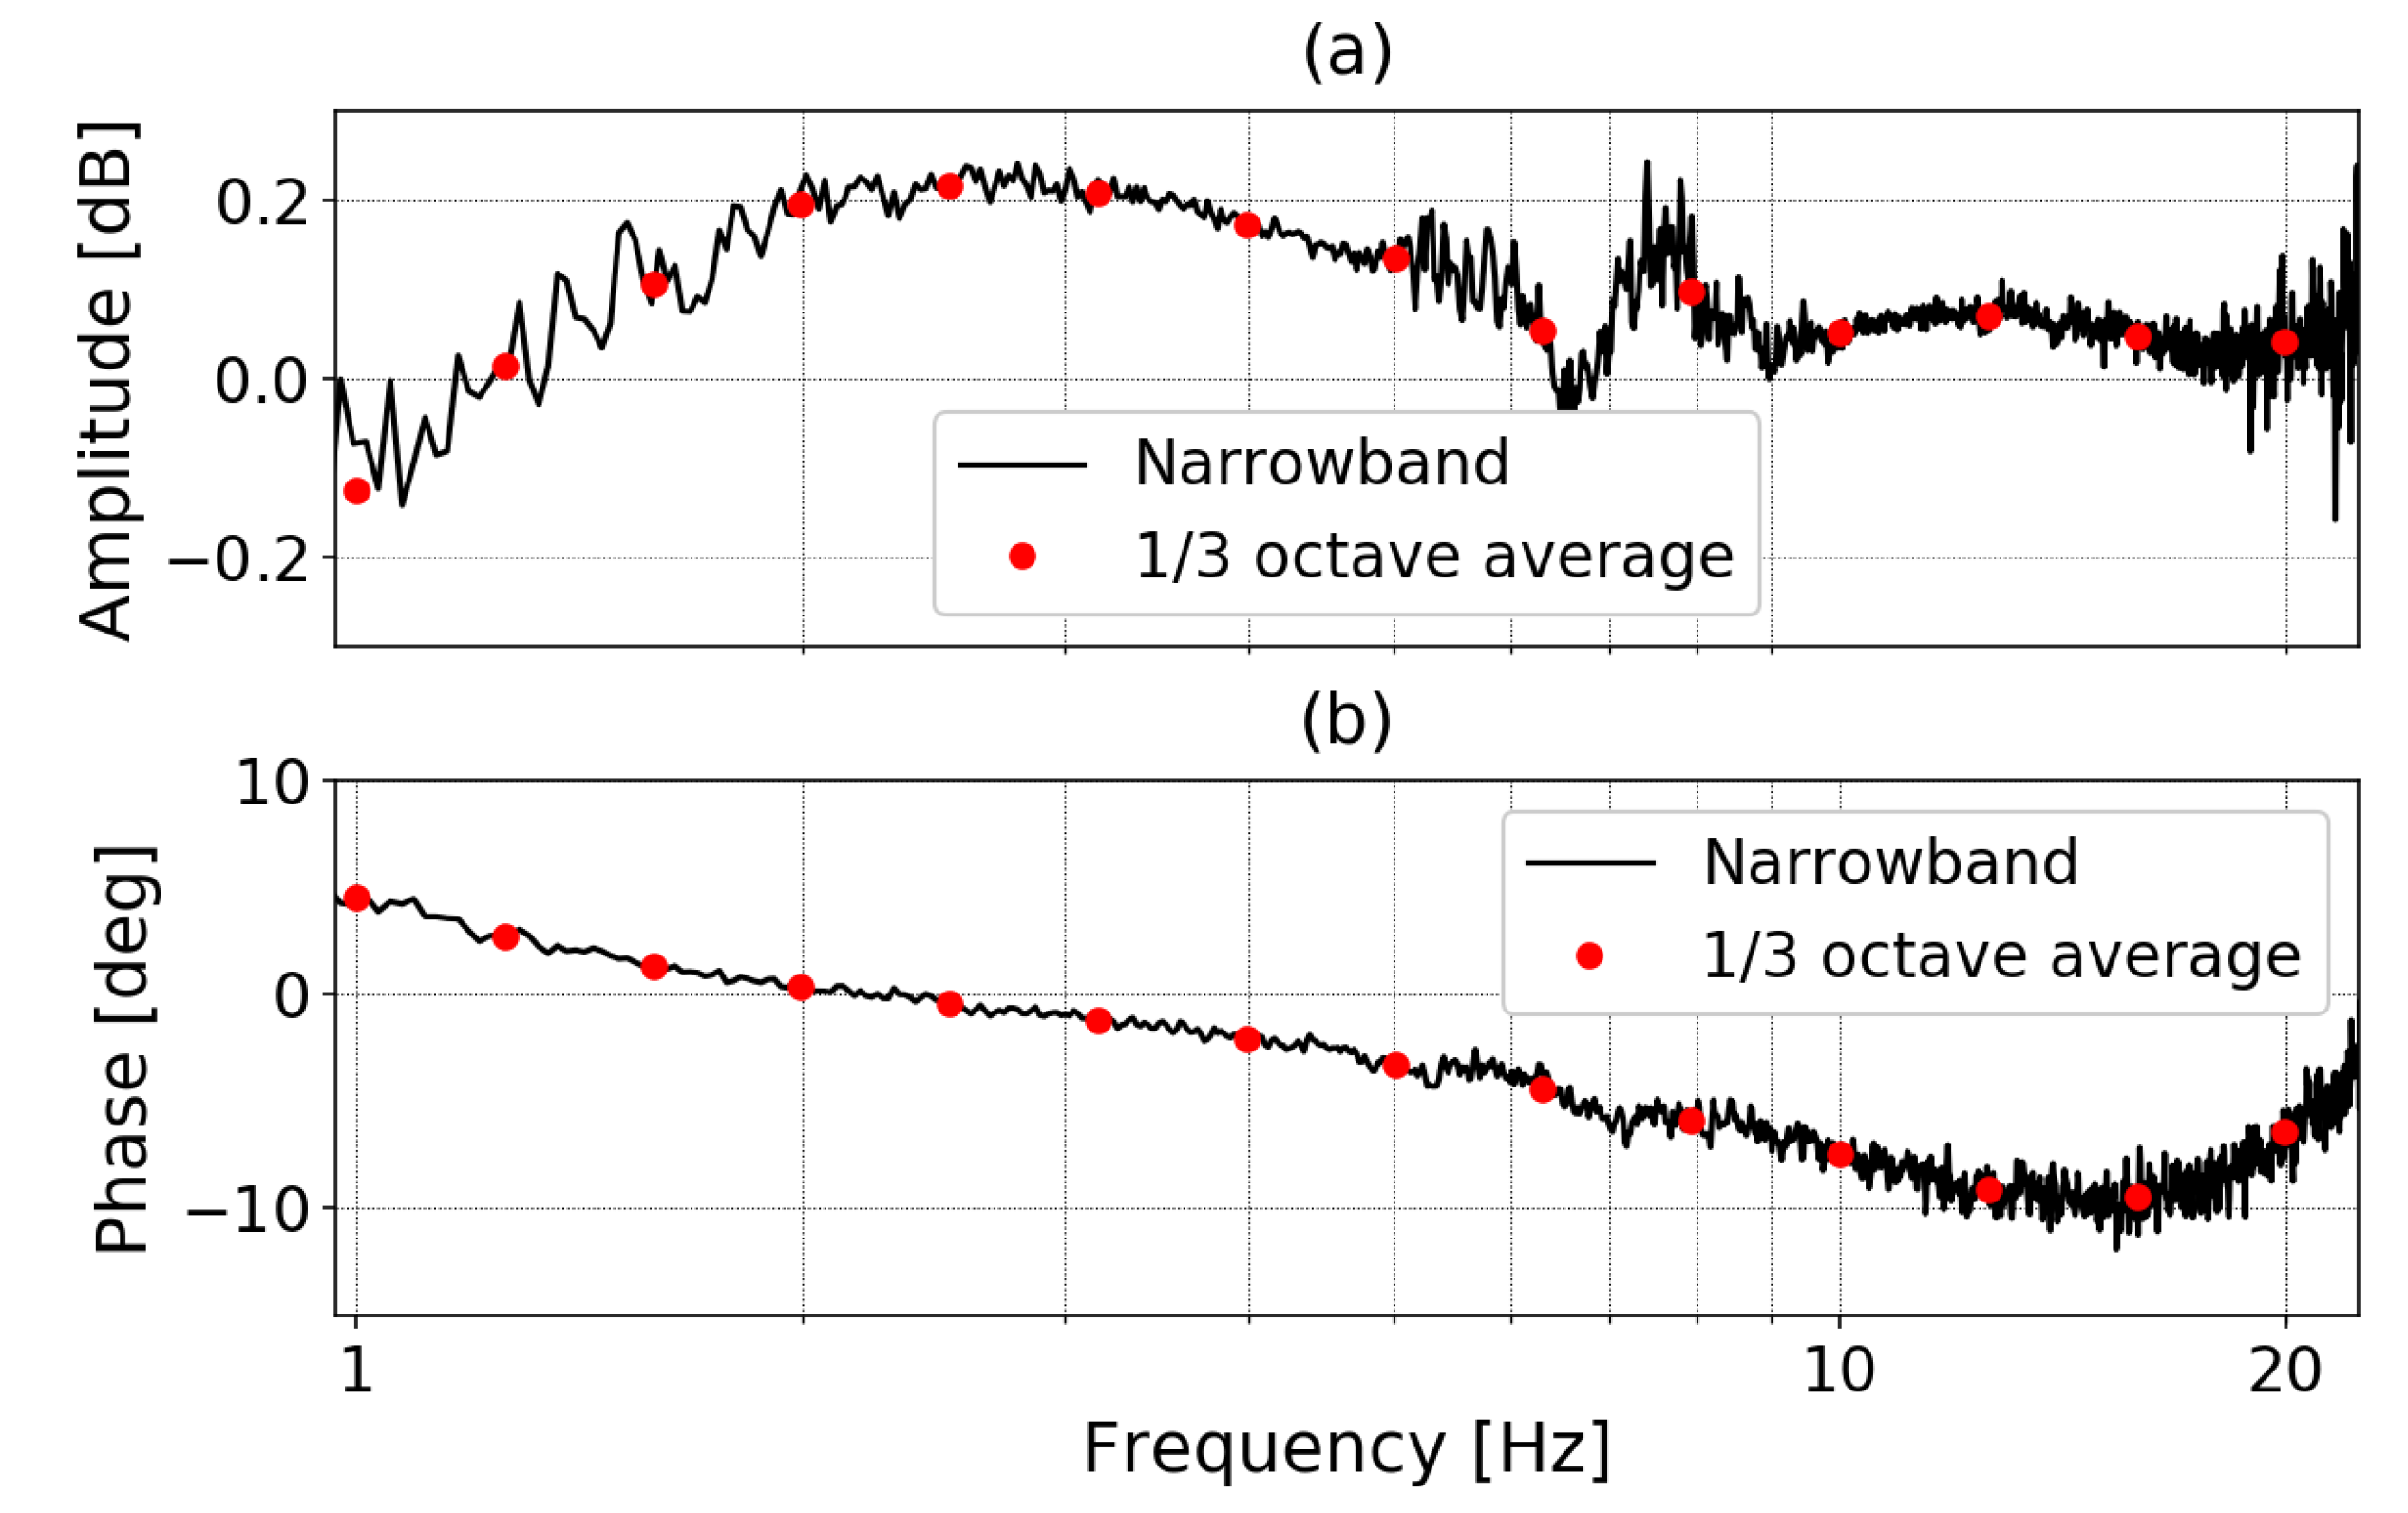
\includegraphics[width=\linewidth]{figures/asmar_3.png}
    \caption{Noise response results for iMic relative to B\&K across 0.97 to 22.4 Hz. (a) Relative amplitude between the sensors, computed as the ratio of their response corrected spectra. (b) Relative phase, computed as the angle of the response corrected cross-spectrum. Raw computations are represented by a solid line, while 1/3-octave band averaging is represented by the filled circles.}
    \label{fig:asmar_3}
\end{figure}

In summary, these results show that distributed mobile devices meet the standards provided by the International Monitoring System (IMS) and can be used to supplement the IMS network with mobile distributed infrasound data. The data recorded by the mobile sensors trend nicely with data collected by ground truth sensors.

This shows that not only are Detections and Incidents accounted for within Lokahi, but the underlying sensors are able to accurately record infrasound levels. Asmar concluded her dissertation by providing methods for calibrating other mobile sensors that don't make use of the iPrecision microphones. These calibration methods have since been adapted and many of Lokahi's other mobile sensors are accurately calibrated to the ground truth sensors.

\section{Results of Generality of this Framework}\label{sec:results-of-generality-of-this-framework}

I have claimed Section~\ref{subsec:generality-of-the-laha-framework} that the Laha framework is general enough to to be suitable for use in multiple domains of DSNs. In the Evaluation chapter~\ref{subsec:evaluation-of-the-generality-of-this-framework}, I provided guidelines for evaluating Laha's generality across the OPQ and Lokahi distributed sensor networks. Next, I will revisit the evaluation guidelines and provide discussion and analysis that provides evidence that the Laha Framework is general enough to be useful in multiple domains while still meeting the requirements of the individual DSNs.

\subsection{Results of Laha Generality for OPQ}\label{subsec:results-of-laha-generality-for-opq}

I claimed in the Evaluation chapter~\ref{subsec:evaluation-of-the-generality-of-this-framework} that the OPQ network must be able to observe common power quality issues including Voltages sags and swells, Frequency sags and swells, excessive THD, and transients. These features were described and shown to exist within OPQ in the previous section on validating collected data by deployments. I will summarize these results here.

Table~\ref{table:incidents_summary} summarizes the relevant Incidents over the three month deployment.

\begin{table}[H]
    \centering
    \caption{Summary of OPQ Incidents}
    \begin{tabularx}{\textwidth}{Xll}
        \toprule
        \textbf{Incident Classification} & \textbf{Total Observed} & \textbf{Mean Observed / Day} \\
        \midrule
        FREQUENCY\_SWELL & 291235 & 3235.94 \\
        FREQUENCY\_SAG & 244286 & 2714.29 \\
        EXCESSIVE\_THD & 21395 & 237.72 \\
        VOLTAGE\_SAG & 620 & 6.89 \\
        ITIC\_NO\_DAMAGE & 93 & 1.03 \\
        SEMI\_F47\_VIOLATION & 24 & 0.27 \\
        VOLTAGE\_INTERRUPTION & 16 & 0.18 \\
        FREQUENCY\_INTERRUPTION & 14 & 0.16 \\
        VOLTAGE\_SWELL & 8 & 0.09 \\
        \bottomrule
    \end{tabularx}
    \label{table:incidents_summary}
\end{table}

As can be observed, Laha was able to detect the types of Incidents as defined by the Evaluation chapter. I will now examine several of these Incidents in greater detail.

\subsubsection{Example OPQ Incidents}

Figure~\ref{fig:vsag_semi_itic} shows a Voltage sag with associated Semi-F47 and ITIC violations. Note, this is the only such Incident where the Voltage sag created both a Semi-F47 violation and an ITIC violation. This occurred during a power outage on the UHM campus on November 9, 2019.

\begin{figure}[H]
    \centering
    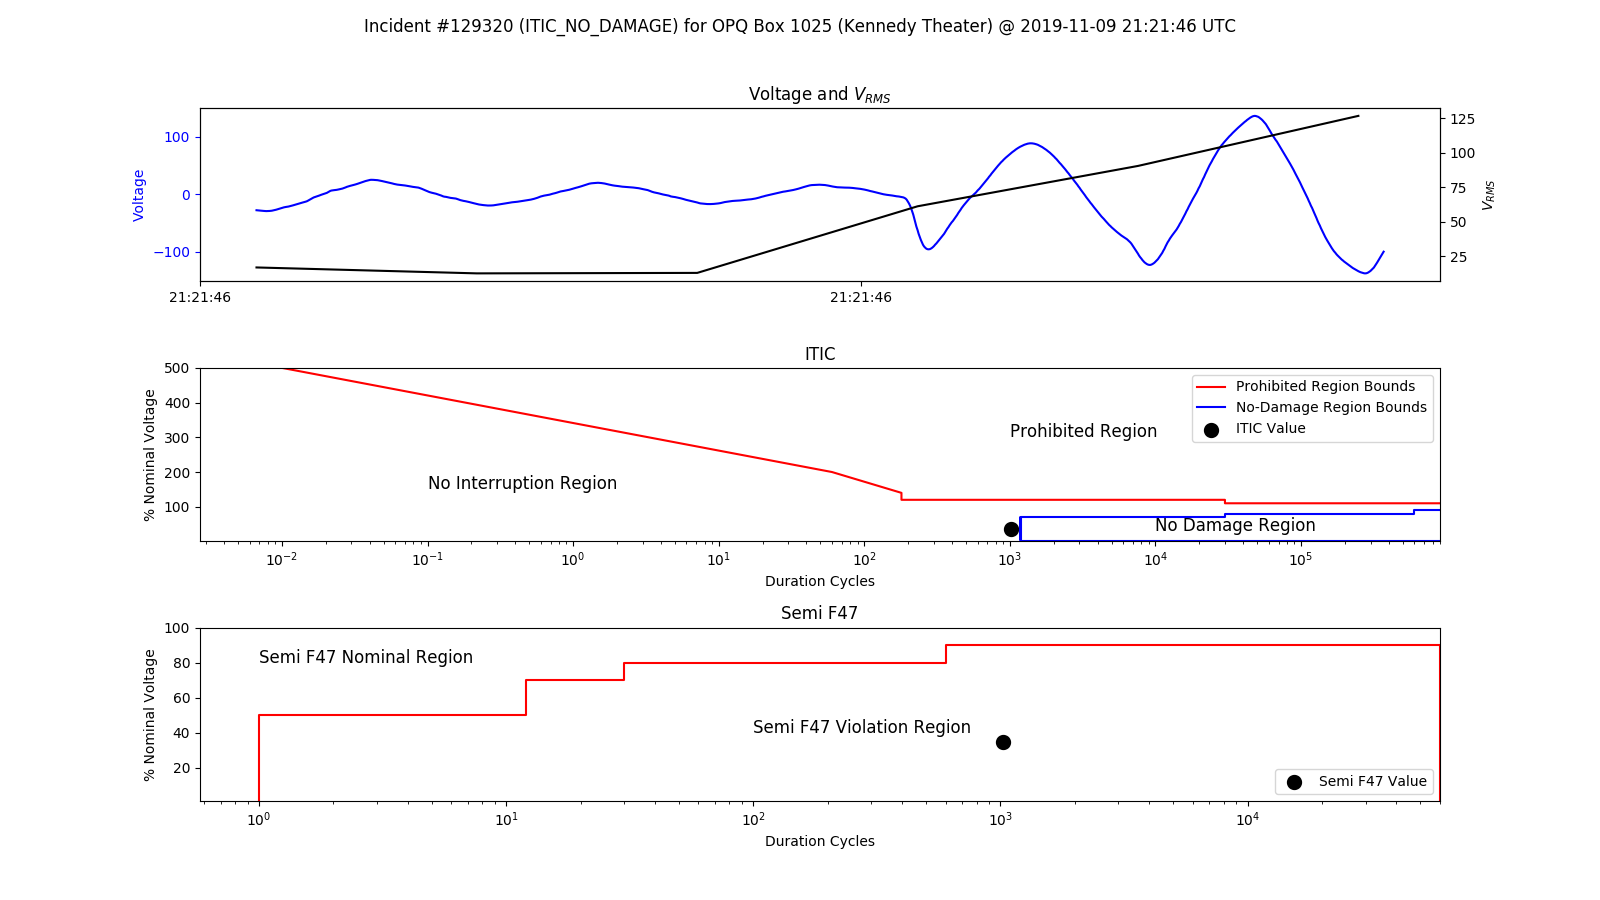
\includegraphics[width=\linewidth]{figures/semi_itic.png}
    \caption{Voltage Sag with Associated Semi-F47 and ITIC Violation}
    \label{fig:vsag_semi_itic}
\end{figure}

Here, the initial voltage waveform and $V_{RMS}$ show a sag on the order of $10^3$ cycles. This is just long enough in duration and low enough in Voltage that is breaches the Semi-F47 threshold and barely surpasses the ITIC threshold.

Figure~\ref{fig:vsag_semi} provides an example of both a large Voltage sag and a related Semi-47 violation, but no ITIC violation. This is much more common in the data.

\begin{figure}[H]
    \centering
    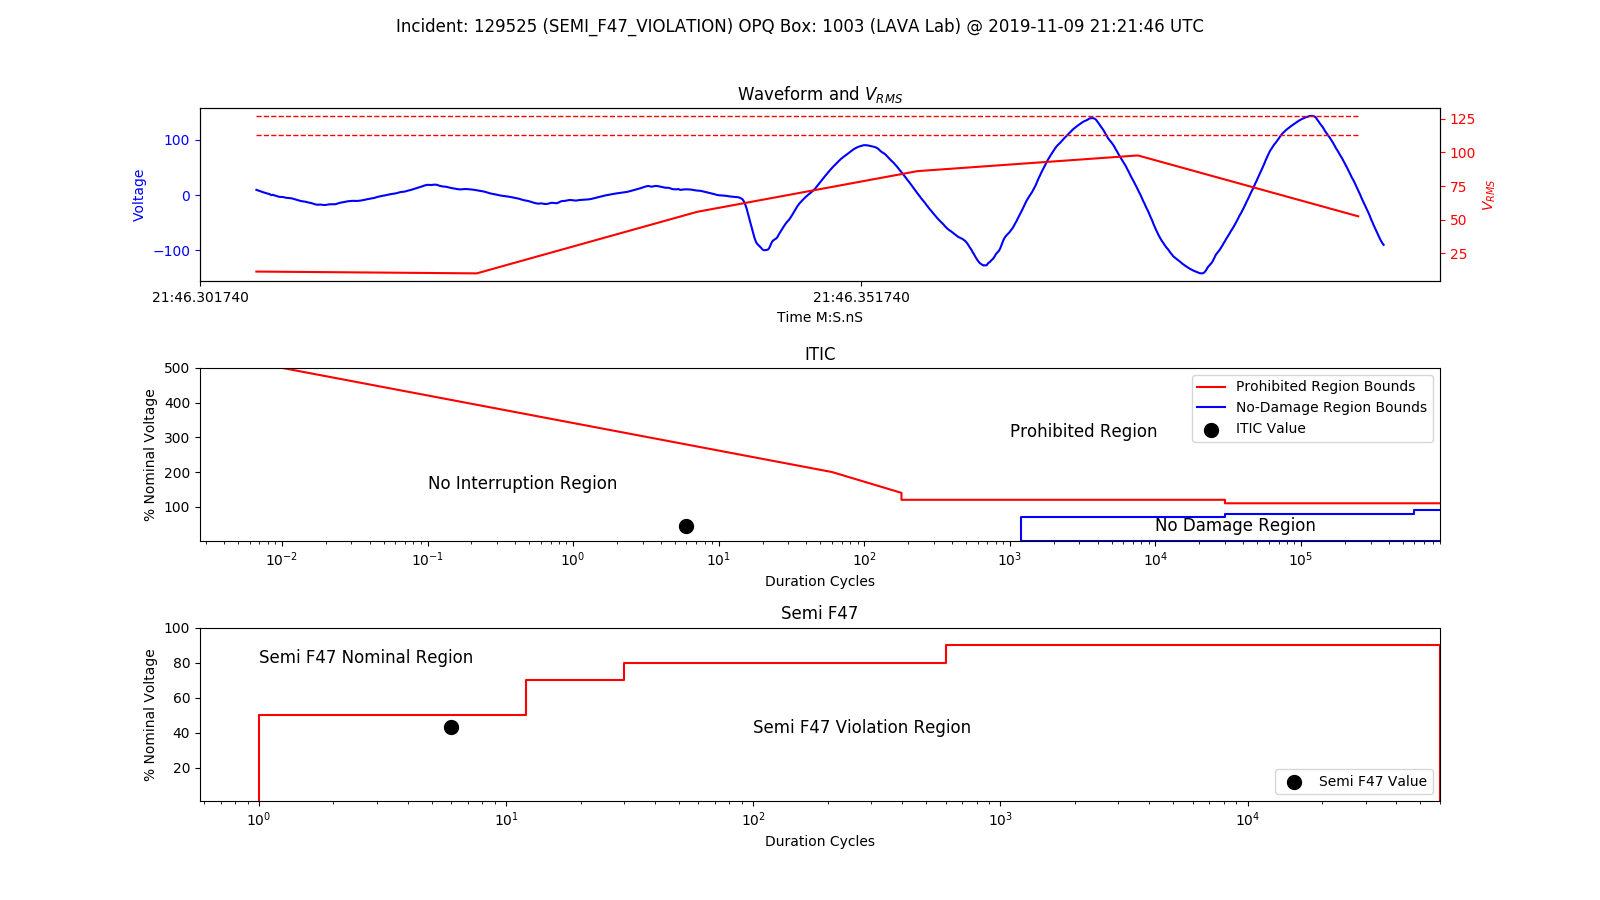
\includegraphics[width=\linewidth]{figures/voltage-incident-129525.png}
    \caption{Voltage Sag with Associated Semi-F47 Violation}
    \label{fig:vsag_semi}
\end{figure}

Figures~\ref{fig:vsag_1} and~\ref{fig:vsag_2} show a Voltage sag that was observed by multiple OPQ Boxes.

\begin{figure}[H]
    \centering
    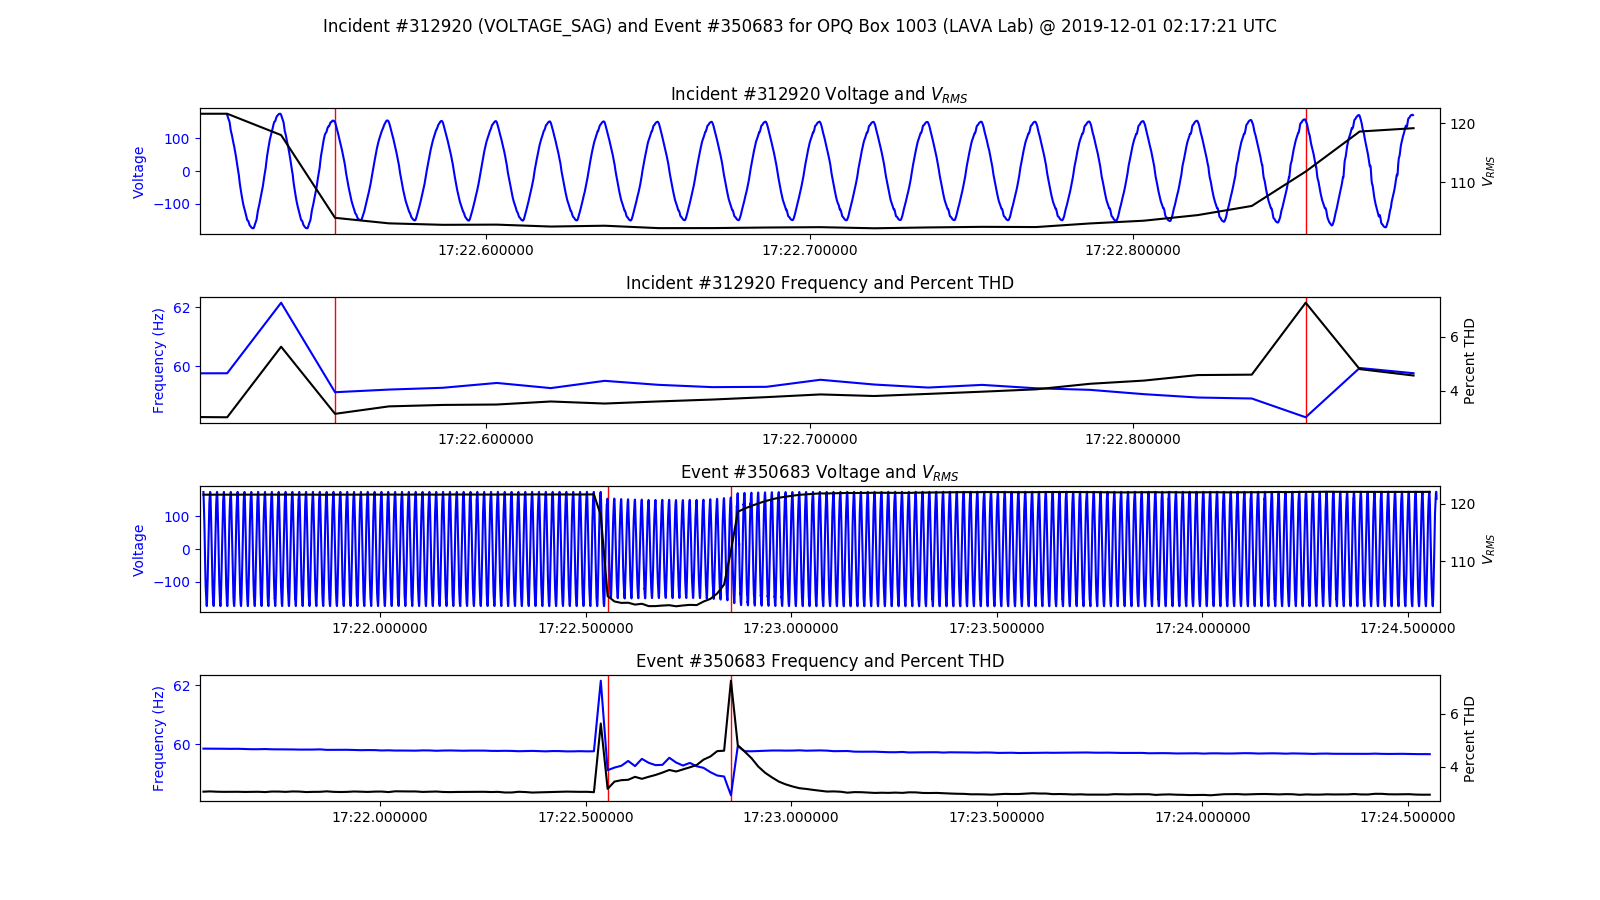
\includegraphics[width=\linewidth]{figures/vsag_1.png}
    \caption{Co-Observed Voltage Sag A}
    \label{fig:vsag_1}
\end{figure}

\begin{figure}[H]
    \centering
    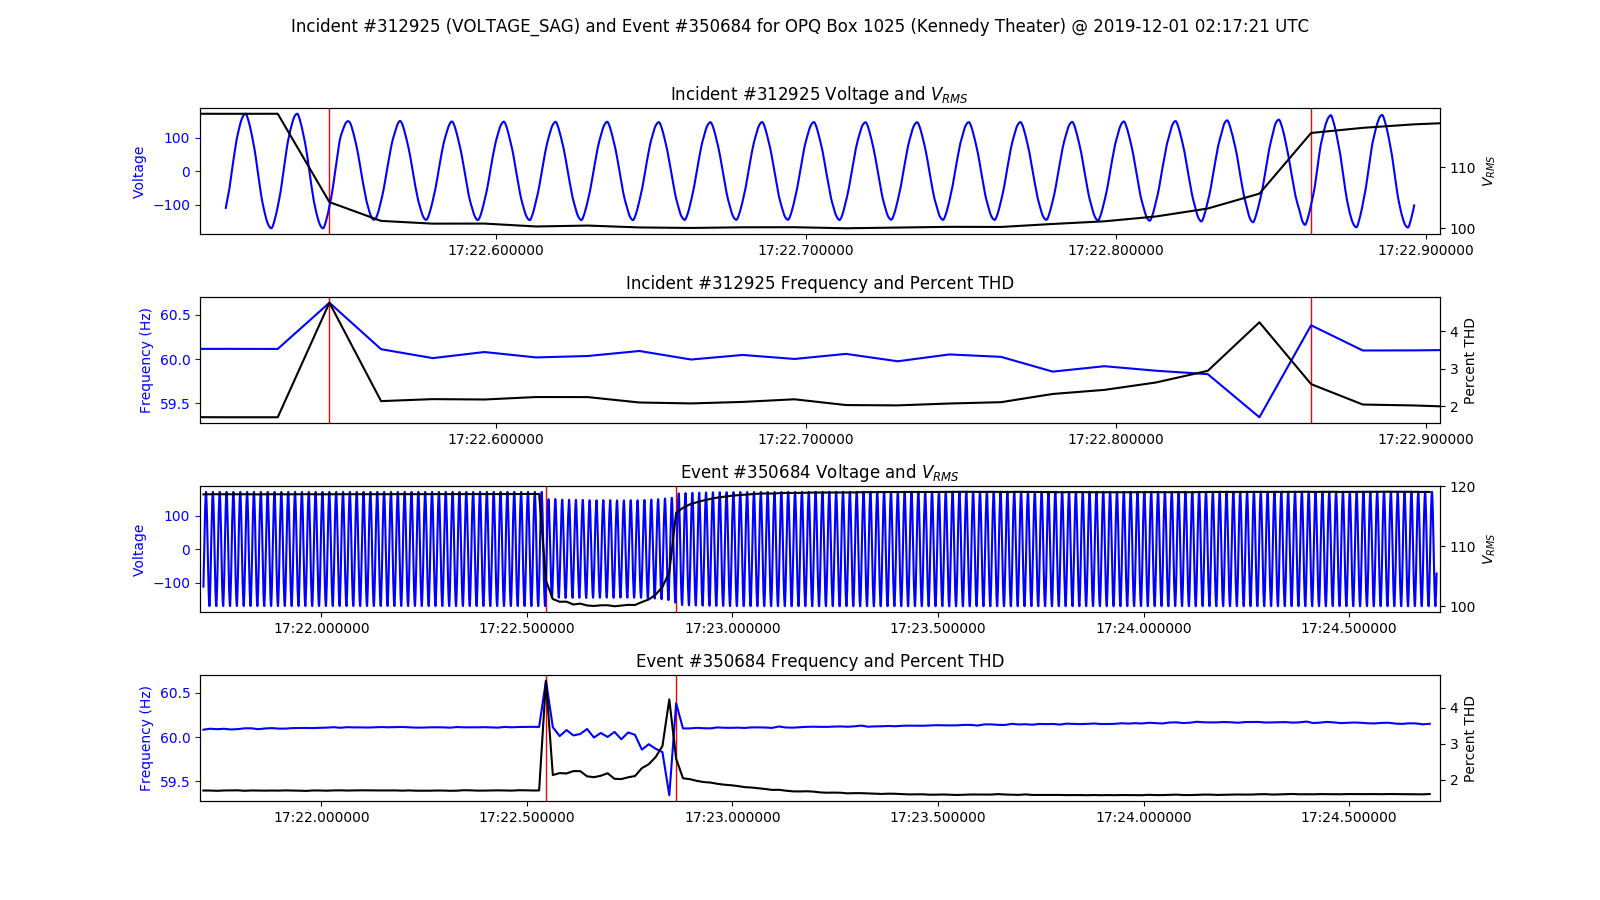
\includegraphics[width=\linewidth]{figures/vsag_2.png}
    \caption{Co-Observed Voltage Sag B}
    \label{fig:vsag_2}
\end{figure}

These two figures show a semi-global Incident that was detected by two OPQ Boxes. The first Box was located Keller while the other was located in Kennedy Theater. There are both Voltage and Frequency deviations that were tracked by both Boxes.

Figure~\ref{fig:vswell} shows an example of a Voltage swell. You will note that the Semi-F47 does not classify Voltage swells which is why there is a value absent for the bottom panel.

\begin{figure}[H]
    \centering
    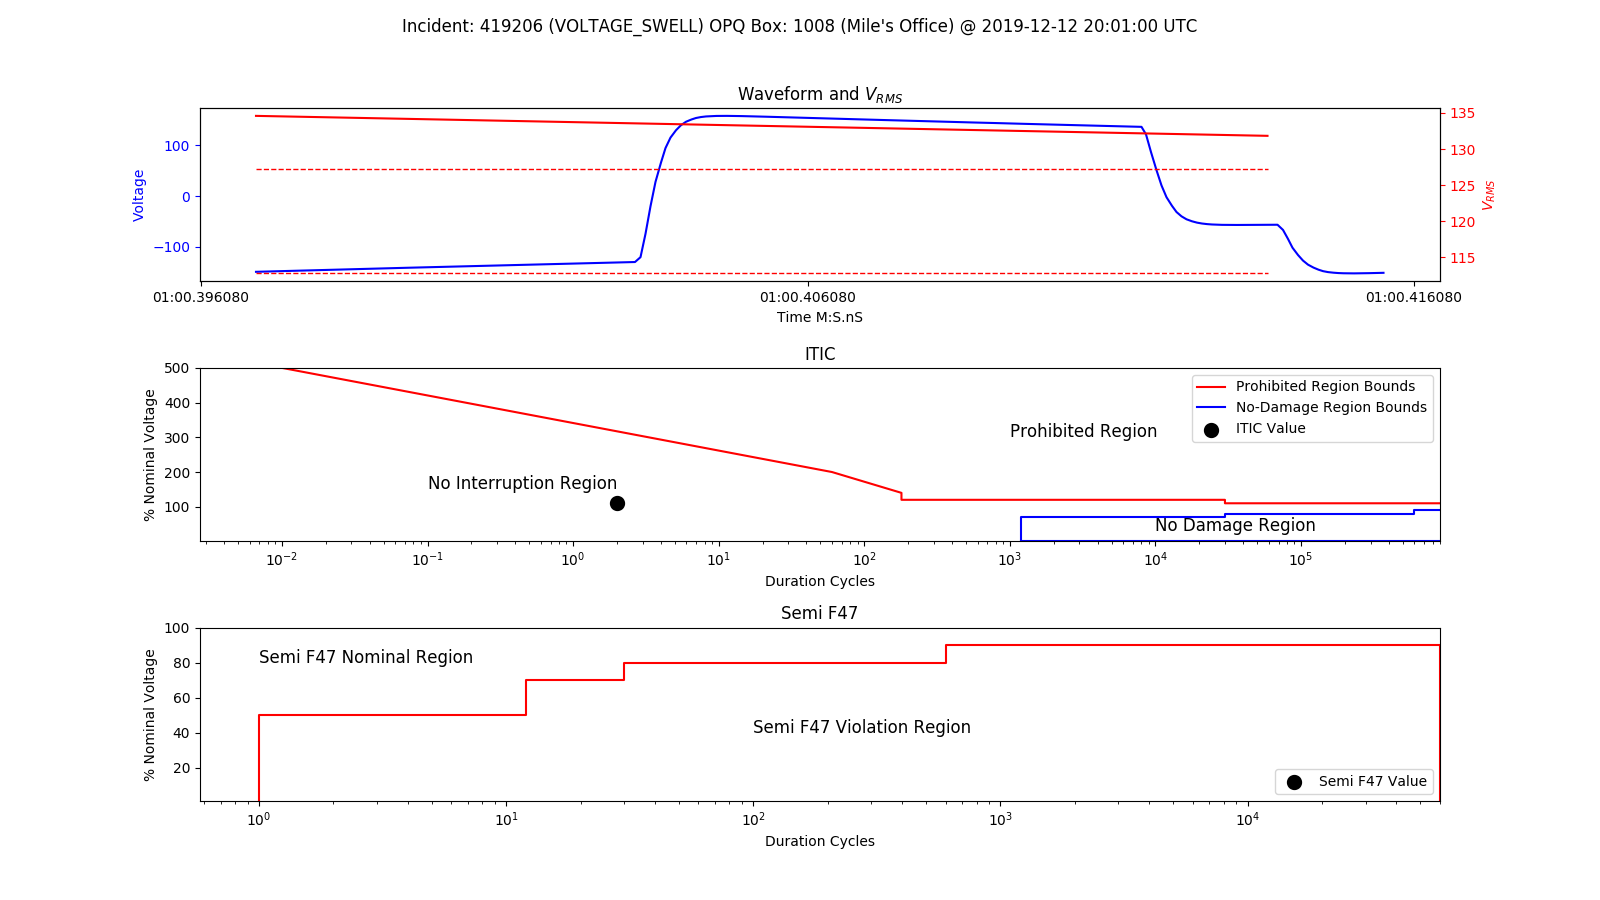
\includegraphics[width=\linewidth]{figures/voltage-incident-419206.png}
    \caption{Voltage Swell}
    \label{fig:vswell}
\end{figure}

Figure~\ref{fig:thd} shows an example of an excessive THD Incident.

\begin{figure}[H]
    \centering
    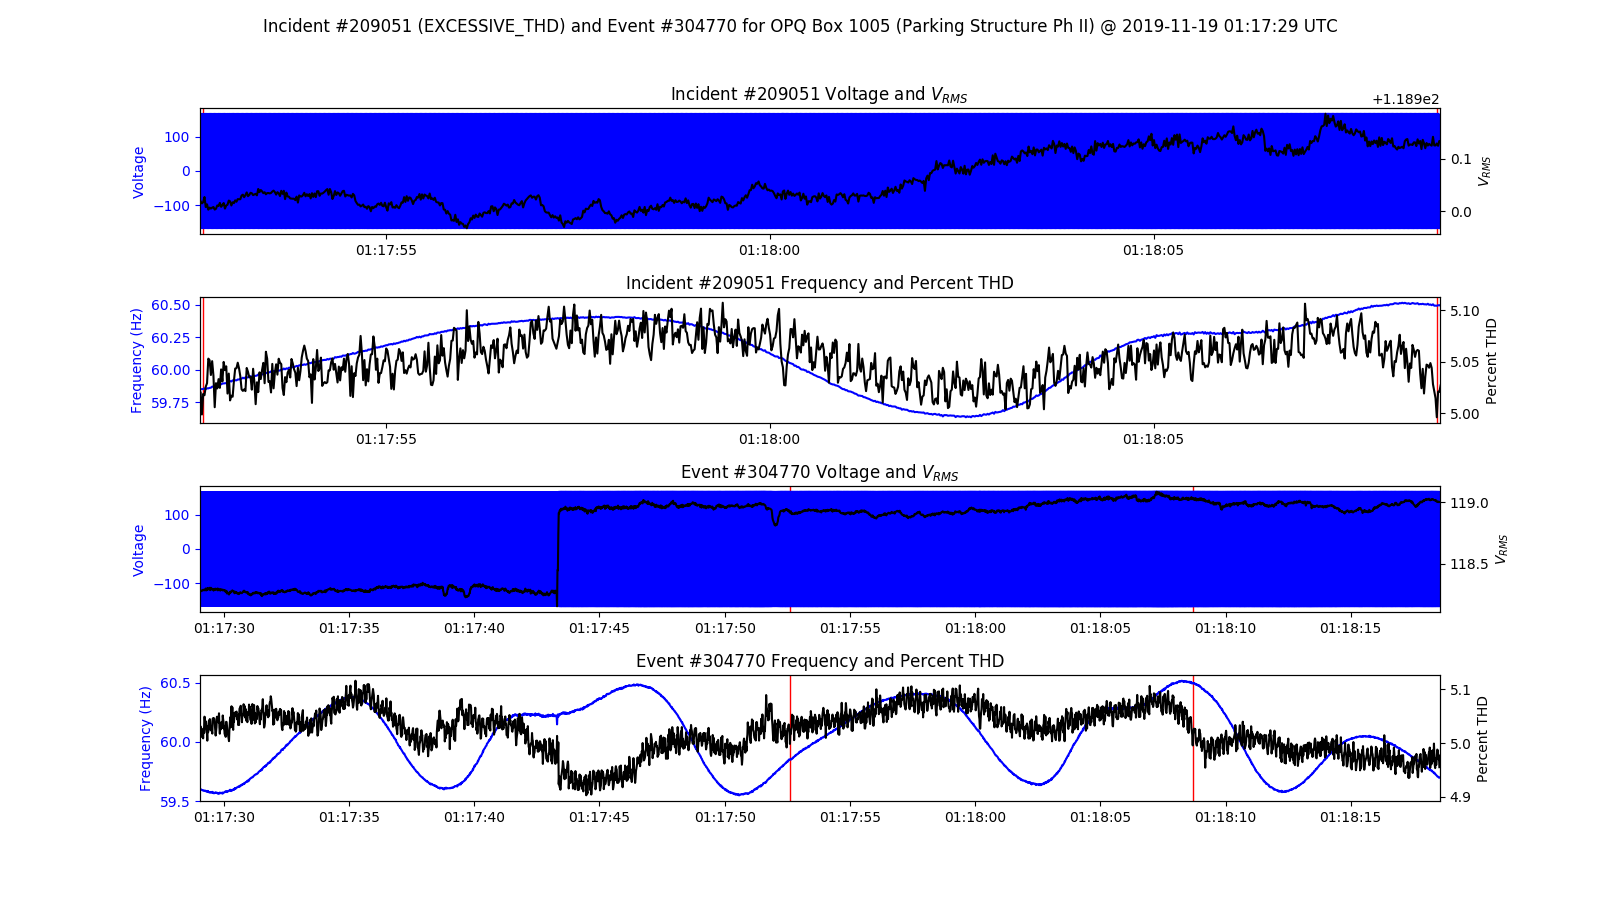
\includegraphics[width=\linewidth]{figures/thd.png}
    \caption{Excessive THD}
    \label{fig:thd}
\end{figure}

THD exceeds 5\% for a period of near 20 seconds.

Figure~\ref{fig:transients} shows an example of a transient that was recorded on Oct 7, 2019.

\begin{figure}[H]
    \centering
    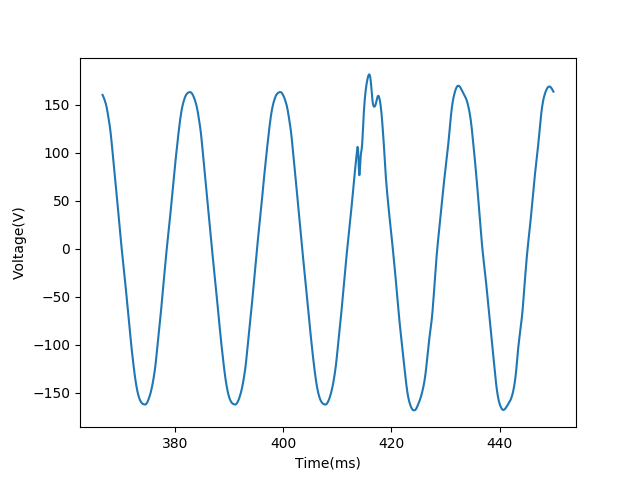
\includegraphics[width=\linewidth]{figures/transient.png}
    \caption{Detected Transients: Box 1001}
    \label{fig:transients}
\end{figure}

Figure~\ref{fig:fsag} shows an example of a Frequency sag.

\begin{figure}[H]
    \centering
    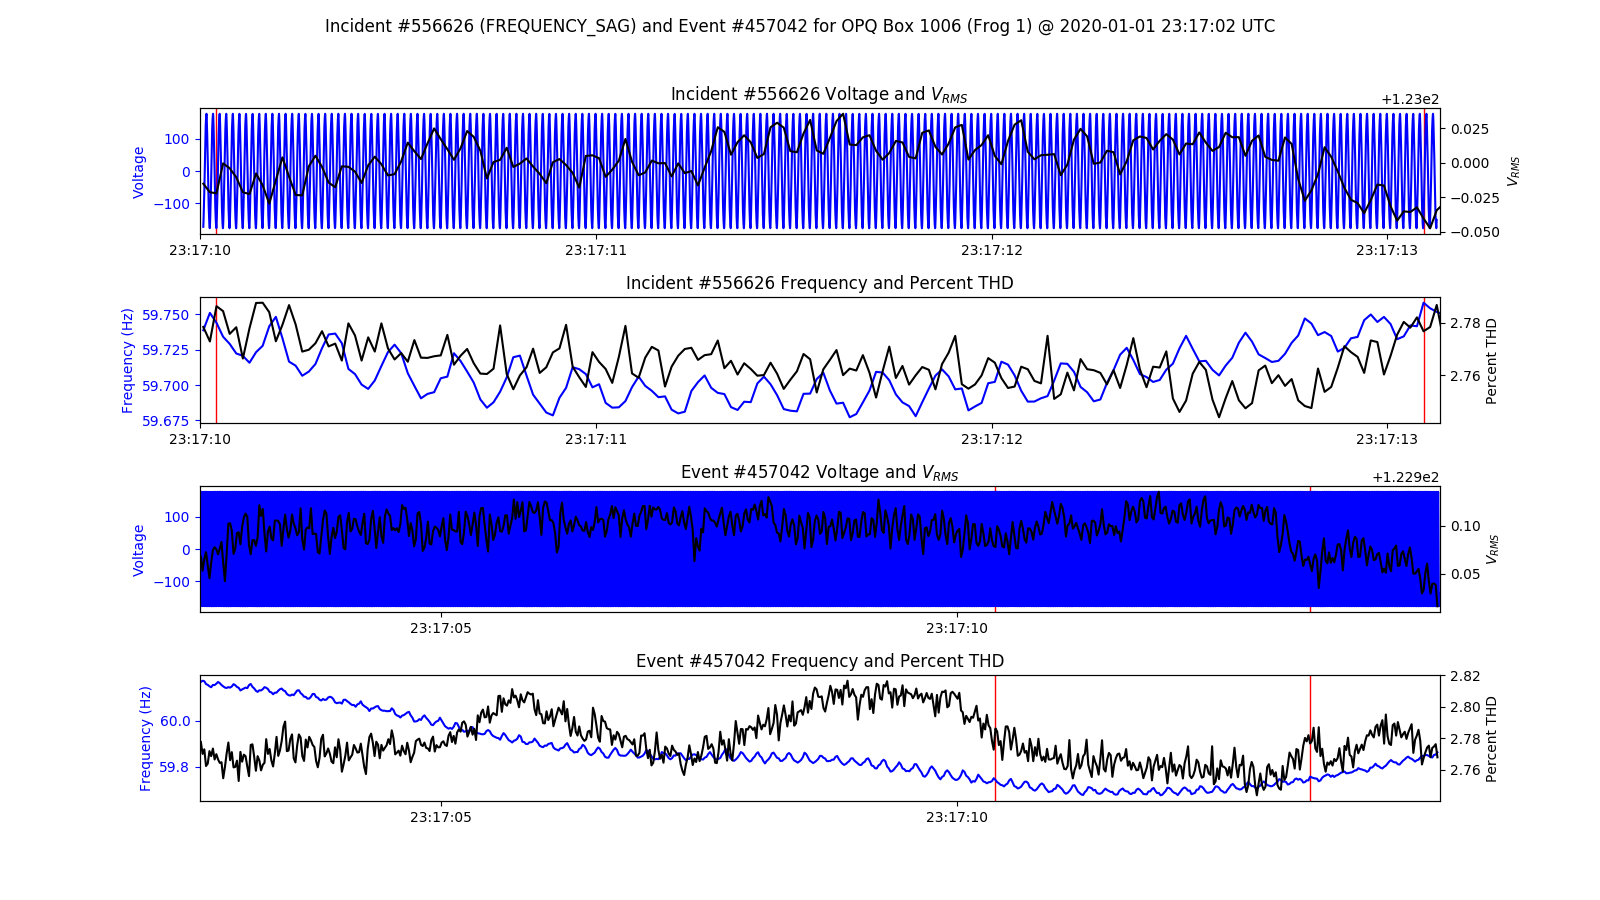
\includegraphics[width=\linewidth]{figures/incident-556626.png}
    \caption{Frequency Sag}
    \label{fig:fsag}
\end{figure}

Figure~\ref{fig:fswell} shows an example of a Frequency swell.

\begin{figure}[H]
    \centering
    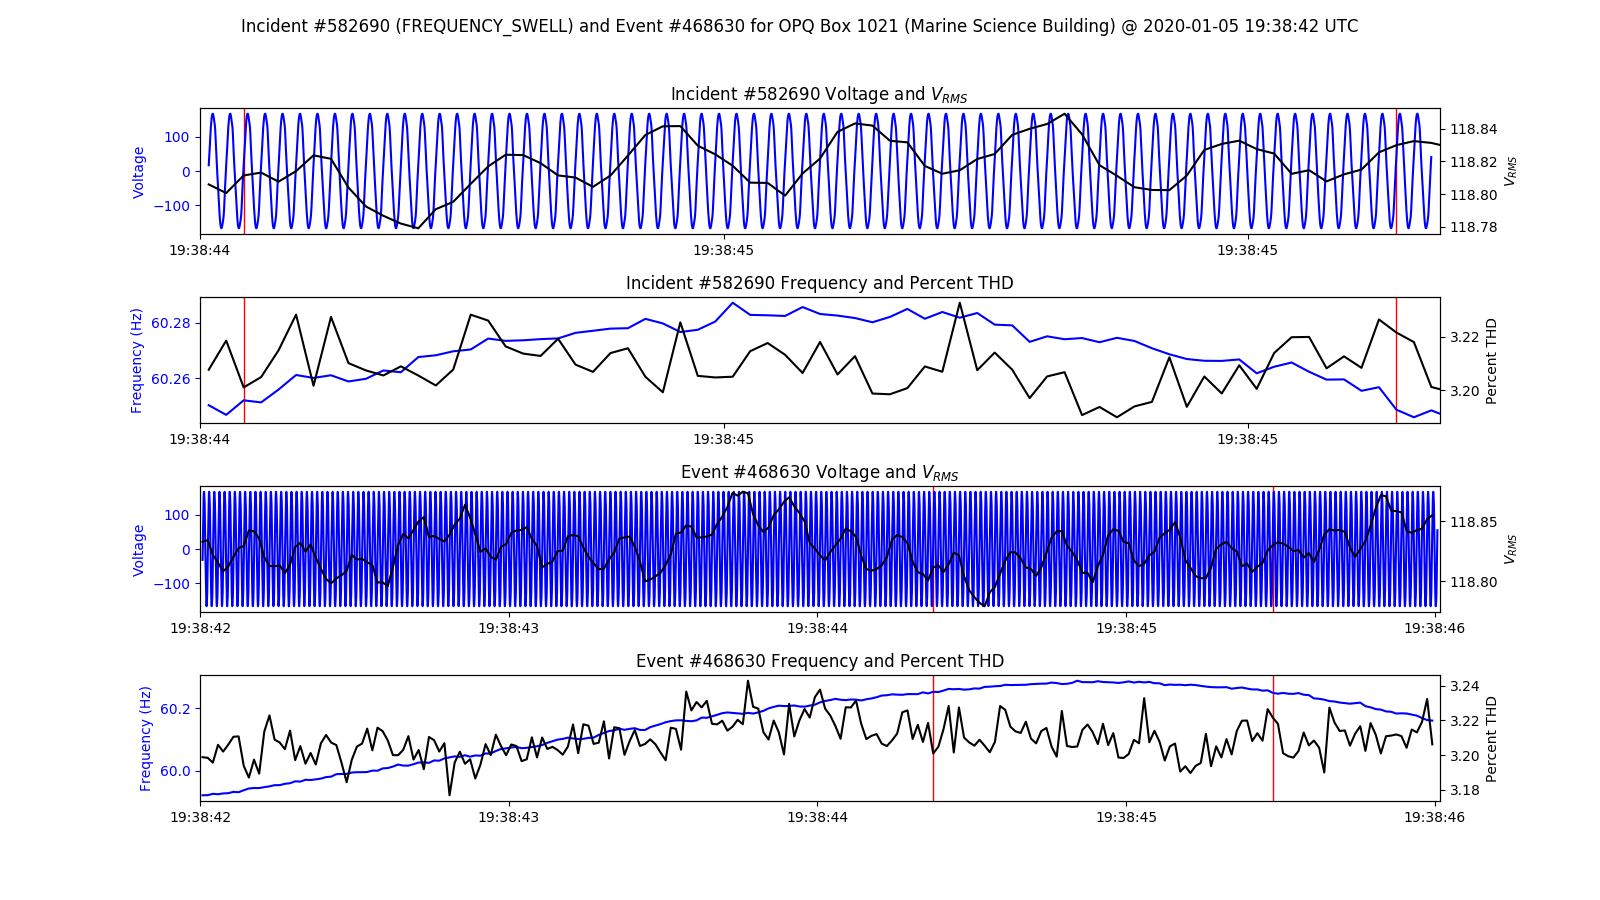
\includegraphics[width=\linewidth]{figures/incident-582690.png}
    \caption{Frequency Swell}
    \label{fig:fswell}
\end{figure}

These examples illustrate a subset of the types of PQ issues that OPQ Mauka is able to detect utilizing the Laha framework. All Incidents are publicly available through OPQ View.

\subsubsection{Local, Semi-Global, and Global Incidents}

I also claimed in the Evaluation chapter that the OPQ network is capable of detecting grid wide signals of interest. I had hoped to see at least one grid wide signal during out deployment, but am happy to report that we actually see many grid wide signals daily. One such way of looking for grid wide signals is to utilize Napali's triggering results (Napali is described in~\cite{napali}). These results provide anomalous signals of interest that were observed by more than one OPQ Box. Table~\ref{table:global_summary} summarizes the number of signals observed by one Box and multiples Boxes.

\begin{table}[H]
    \centering
    \caption{Summary of Global and Semi-Global Events}
    \begin{tabularx}{\textwidth}{ll}
        \toprule
        \textbf{Total Events} & \textbf{Number of Boxes that Observed the Events} \\
        \midrule
        170925 & 1 \\
        1654 & 2 \\
        1109 & 3 \\
        853 & 4 \\
        593 & 5 \\
        416 & 6 \\
        354 & 7 \\
        246 & 8 \\
        203 & 9 \\
        160 & 10 \\
        162 & 11 \\
        130 & 12 \\
        169 & 13 \\
        210 & 14 \\
        477 & 15 \\
        463 & 16 \\
        \bottomrule
    \end{tabularx}
    \label{table:global_summary}
\end{table}

As can be observed, most Events that were triggered were only triggered from a single Box. These were triggered by Mauka's triggering algorithm. All Events that were triggered by more than one Box were triggered by Napali's triggering algorithm. Local Events, or those that were only observed by a single Box make up close to 96\% of the observed Events. The other 4\% are either semi-global or global. We see that 463 of the Events triggered were triggered on all available Boxes and I consider these to be global Events. Events that were triggered by 2 to 15 Boxes I consider semi-global Events.

These results provide evidence that Laha as implemented by OPQ can accurately identify semi-global and global power signals-of-interest.

\subsubsection{Examples of Semi-Global and Global Events}

First, let's look at an example of a semi-global Event as shown in Figures~\ref{fig:sg_events} and~\ref{fig:sg_events_1}.

\begin{figure}[H]
    \centering
    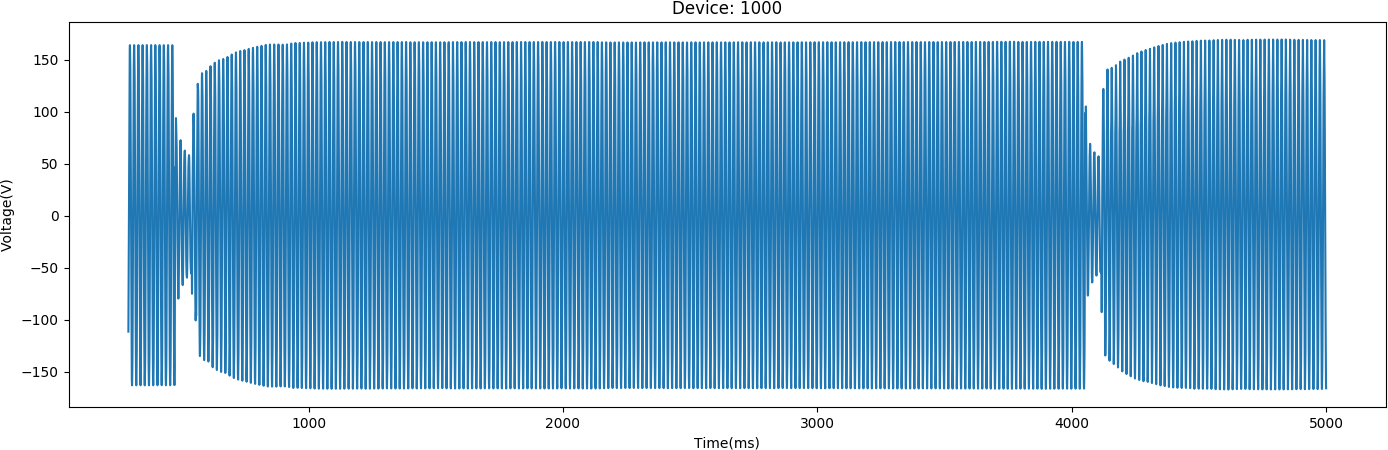
\includegraphics[width=\linewidth]{figures/events_1.png}
    \caption{Semi-Global Events I}
    \label{fig:sg_events}
\end{figure}

\begin{figure}[H]
    \centering
    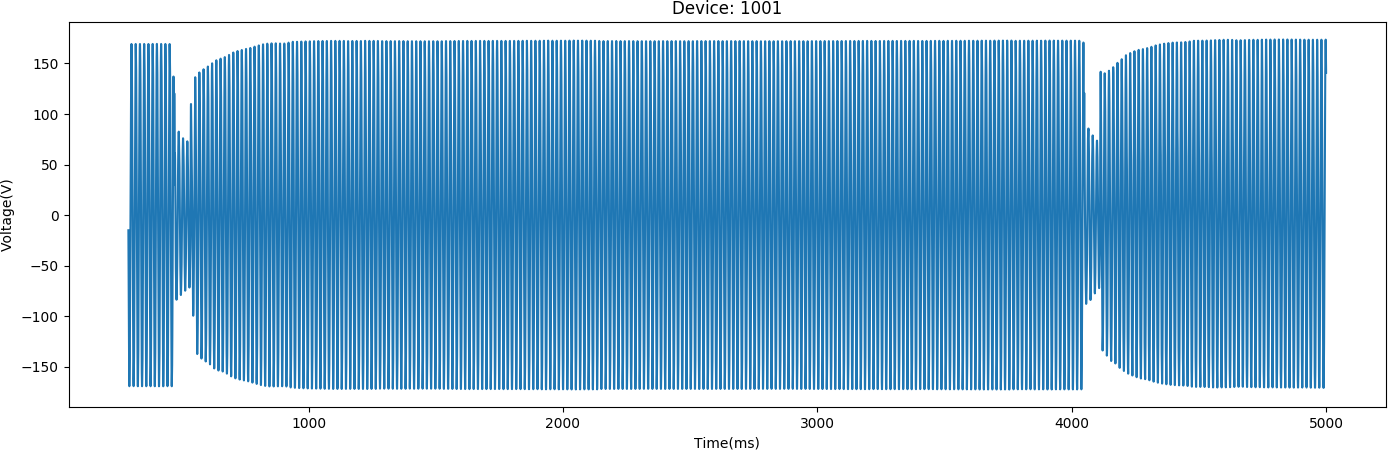
\includegraphics[width=\linewidth]{figures/events_2.png}
    \caption{Semi-Global Events II}
    \label{fig:sg_events_1}
\end{figure}

This collection of Events was recorded on November 9, 2019 and observed by 15 OPQ Boxes over a duration of 5 seconds. There are two Voltages sags that drop to about 80 Volts.  These sags were observed by 15 OPQ Boxes. I only show two devices above for brevity. The rest look similar.

Next, let's examine an example of a semi-global Incident. Figure~\ref{fig:i_1} and Figure~\ref{fig:i_2} show examples of a Voltage sag Incident observed across 7 OPQ Boxes on November 23, 2019.

\begin{figure}[H]
    \centering
    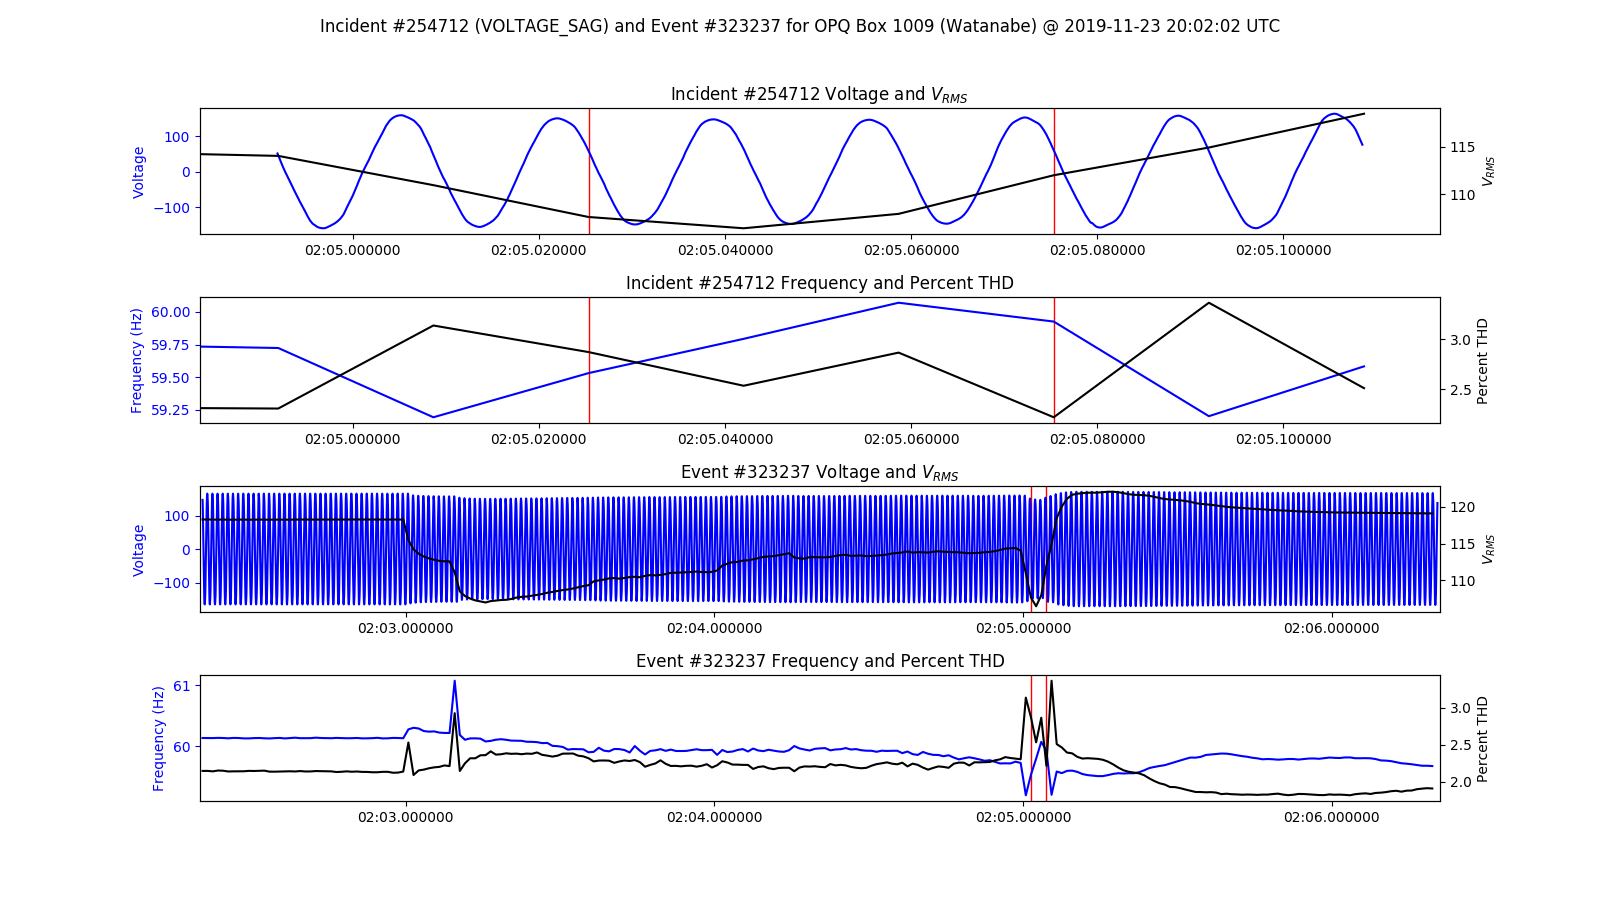
\includegraphics[width=\linewidth]{figures/vsag_g_1.png}
    \caption{Semi-Global Incidents I}
    \label{fig:i_1}
\end{figure}

\begin{figure}[H]
    \centering
    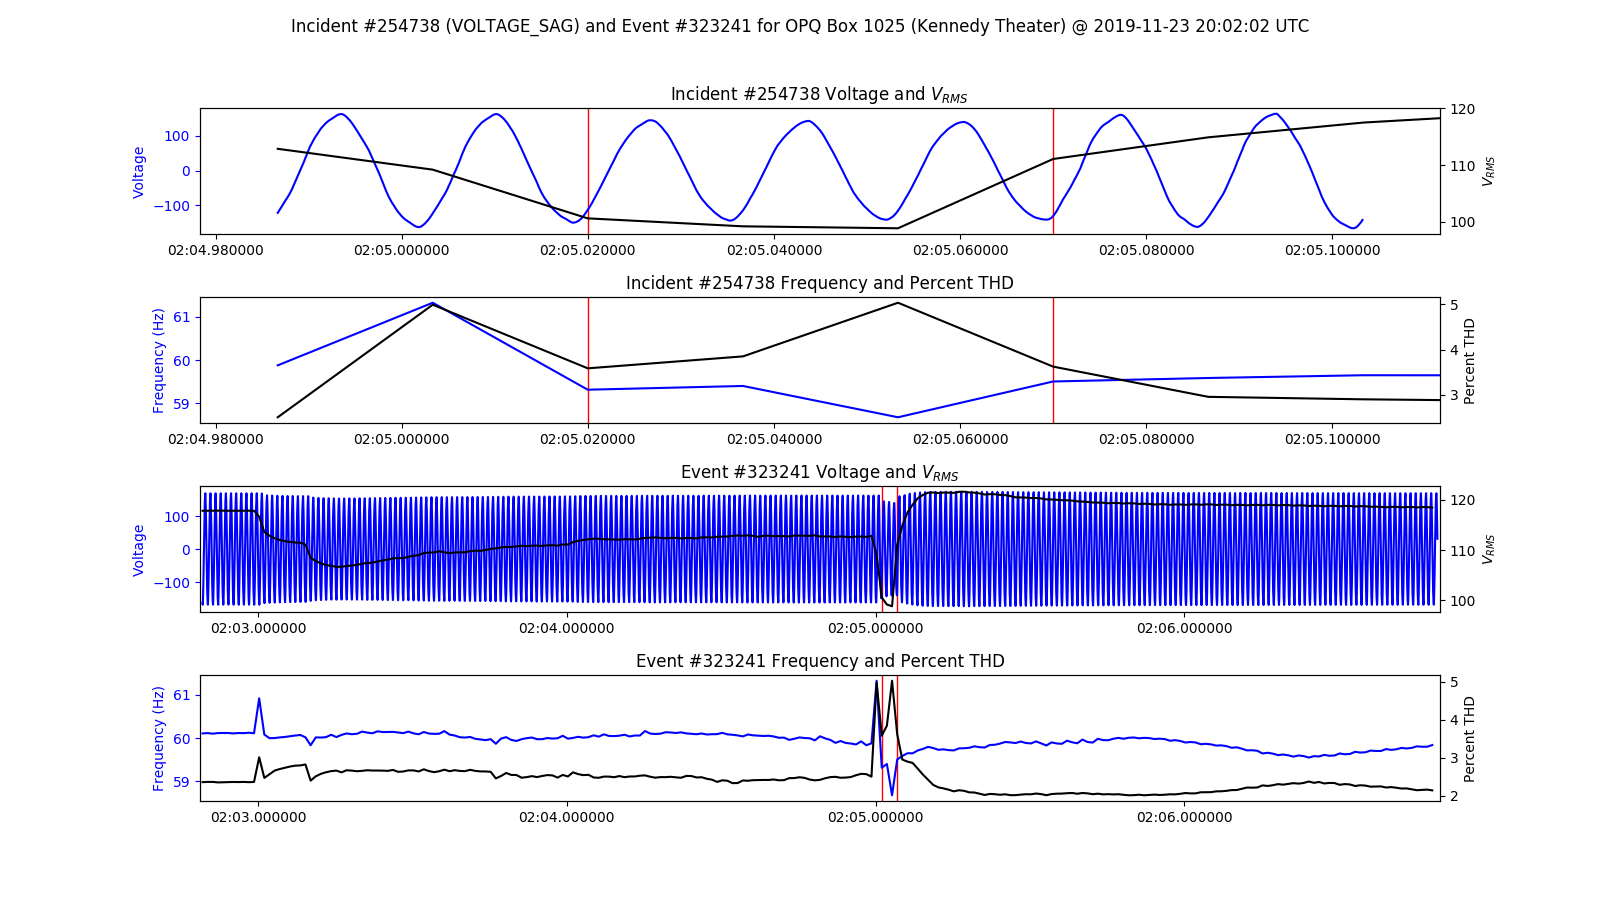
\includegraphics[width=\linewidth]{figures/vsag_g_2.png}
    \caption{Semi-Global Incidents II}
    \label{fig:i_2}
\end{figure}

Here, each Box observes a sag of down to near 100 Volts. You'll note other Voltage sags in the Event waveform. These were also classified as semi-global Incidents. Only two Boxes are shown for brevity.

In summary, I've shown examples of several interesting semi-global Events and Incidents.

\subsubsection{Summary of Laha Generality for OPQ}

In this section, I showed that the OPQ network meets and surpasses the minimum requirements set out in the Evaluation chapter to show the generality of the Laha framework as implemented by OPQ. I showed that OPQ is able to detect common PQ issues and also showed that it is able to detect semi-global and global signals-of-interest.

\subsection{Results of Laha Generality for Lokahi}\label{subsec:results-of-laha-generality-for-lokahi}

I claimed in the Evaluation chapter~\ref{subsec:evaluation-of-the-generality-of-this-framework} that the Lokahi infrasound network is able to securely detect infrasonic signals of interest from a wide variety of heterogeneous mobile devices. The Lokahi network has successfully detected many signatures of interest with different modalities. These include rocket launches, aircraft operations, explosions, and signals created from objects reentering the Earth's atmosphere.

I will now summarize and showcase some of the most interesting data that was collected from Lokahi that meets the requirements set forth in the Evaluation chapter. In particular, I hope to show that Lokahi is able to detect infrasonic signals generated from a diverse set of sources.


\subsubsection{Big Island Earth Quake}
Figures~\ref{fig:quake_1} and~\ref{fig:quake_2} show a magnitude 4.5 earth quake (USGS\cite{usgs_quake}) that was detected in the infrasound range and by accelerometers on the Big Island of Hawaii on August 12 2019. The earth quake was observed by four sensors. I show only one sensor here (and the rest of this section) for brevity. The full results for all examples are publicly available online\cite{redvox_reports}.

\begin{figure}[H]
    \centering
    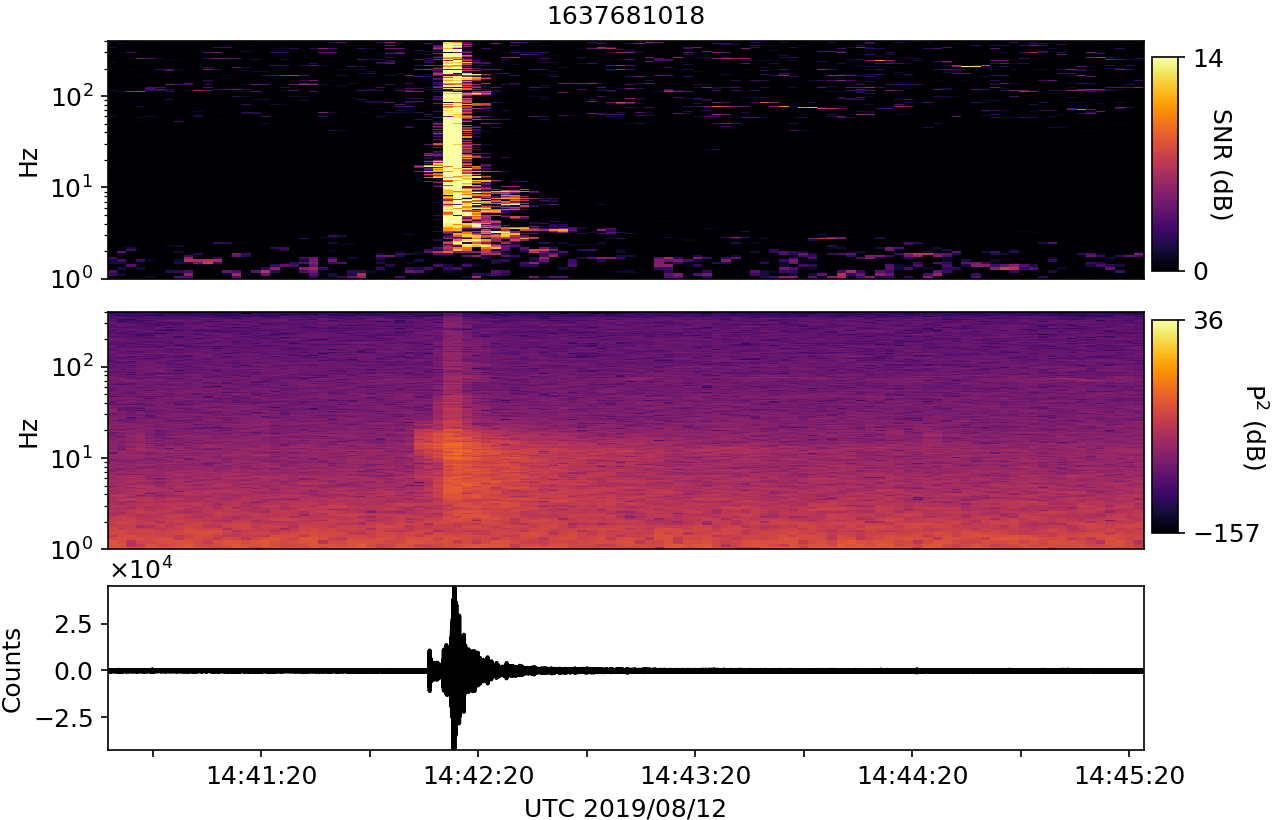
\includegraphics[width=\linewidth]{figures/quake_1.png}
    \caption{Infrasound of Earth Quake}
    \label{fig:quake_1}
\end{figure}

The above Figure shows the infrasound spike created by the earth quake.

\begin{figure}[H]
    \centering
    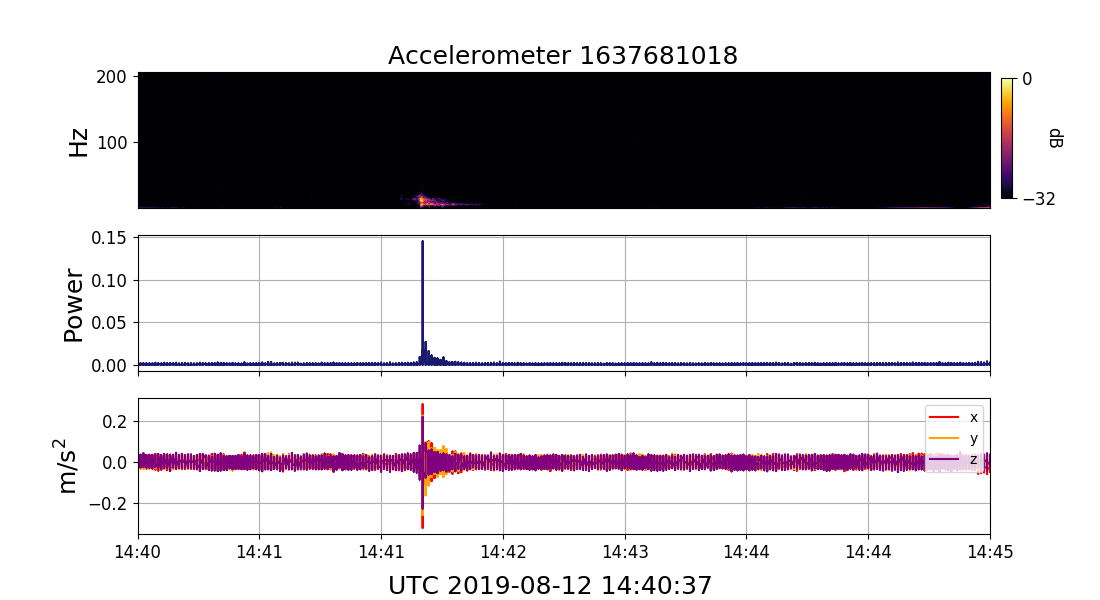
\includegraphics[width=\linewidth]{figures/quake_2.png}
    \caption{Accelerometer of Earth Quake}
    \label{fig:quake_2}
\end{figure}

The above Figure shows the anomalous accelerometer readings during the earth quake.

Figure~\ref{fig:quake_3} shows the map of the earth quake epicenter (in red) and the location of the sensors (white are iPhones and green are Android phones) when the earthquake occurred.

\begin{figure}[H]
    \centering
    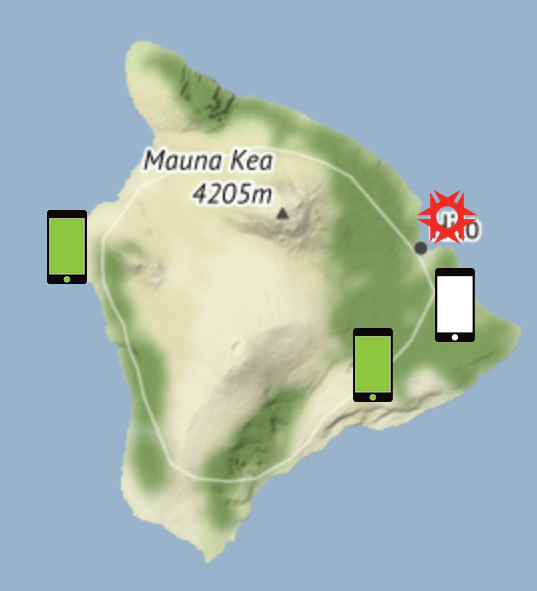
\includegraphics[width=.50\linewidth]{figures/quake_3.png}
    \caption{Location of Earth Quake and Sensors}
    \label{fig:quake_3}
\end{figure}

It should be noted that there are two sensors on top of each other in Kailua-Kona that are not visible in the above map.

\subsubsection{Meteor Entry Over Hawaiian Islands}
On July 25 2019, a meteor entered the atmosphere above the Hawaiian islands as reported by the American Meteor Society\cite{ams}. The Lokahi network observed the event on 19 sensors stationed on the islands of Oahu, Maui, and the Big Island.

Figure~\ref{fig:meteor_1} shows the infrasound as recorded by device 1637610019:1472585716. A large spike can be observed in the infrasound range showing the meteor entering Earth's atmosphere.

\begin{figure}[H]
    \centering
    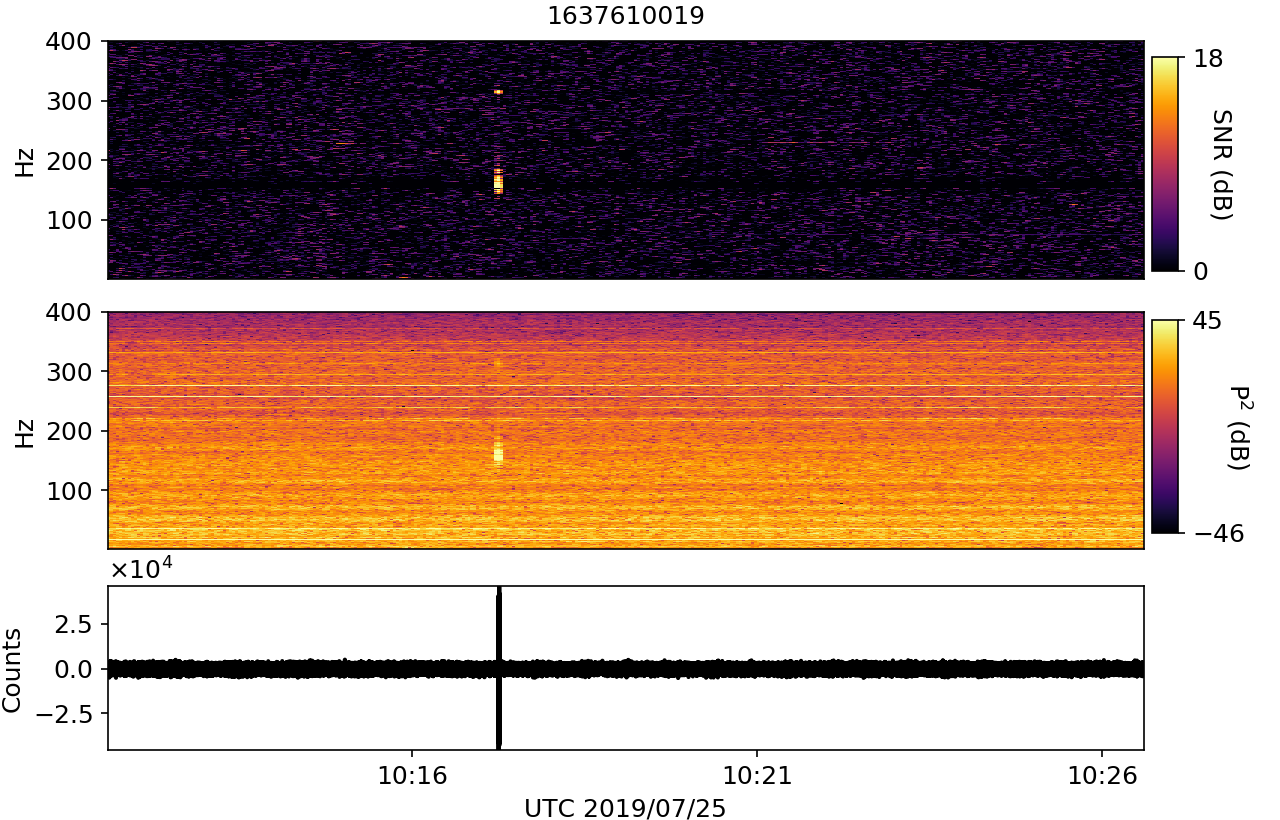
\includegraphics[width=\linewidth]{figures/meteor_1.png}
    \caption{Infrasound of Meteor Entry}
    \label{fig:meteor_1}
\end{figure}

Figure~\ref{fig:meteor_2} shows the locations of sensors that observed the meteor entry.

\begin{figure}[H]
    \centering
    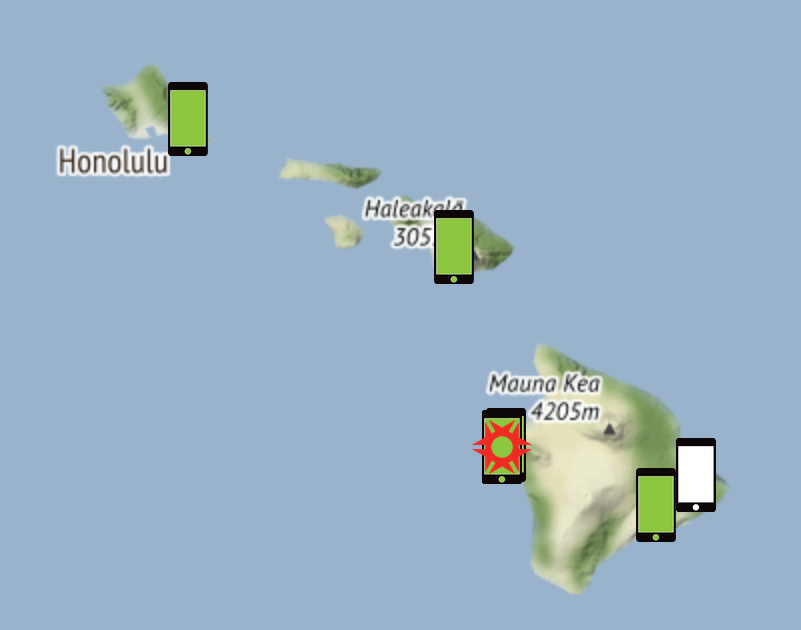
\includegraphics[width=.75\linewidth]{figures/meteor_2.png}
    \caption{Meteor Entry Sensor Locations}
    \label{fig:meteor_2}
\end{figure}

\subsubsection{Falcon 9 Launch and First Stage Landing}

On November 11 2019, SpaceX launched its Falcon 9 rocket on a mission to deploy 60 Starlink satellites\cite{spacex}. The Lokahi network observed the launch and landing of the fist stage on a barge off the coast of Florida in the infrasound range with four sensors located near Cape Canaveral, Florida.

Figure~\ref{fig:spacex_1} shows the infrasound signal for the launch and the first stage landing.

\begin{figure}[H]
    \centering
    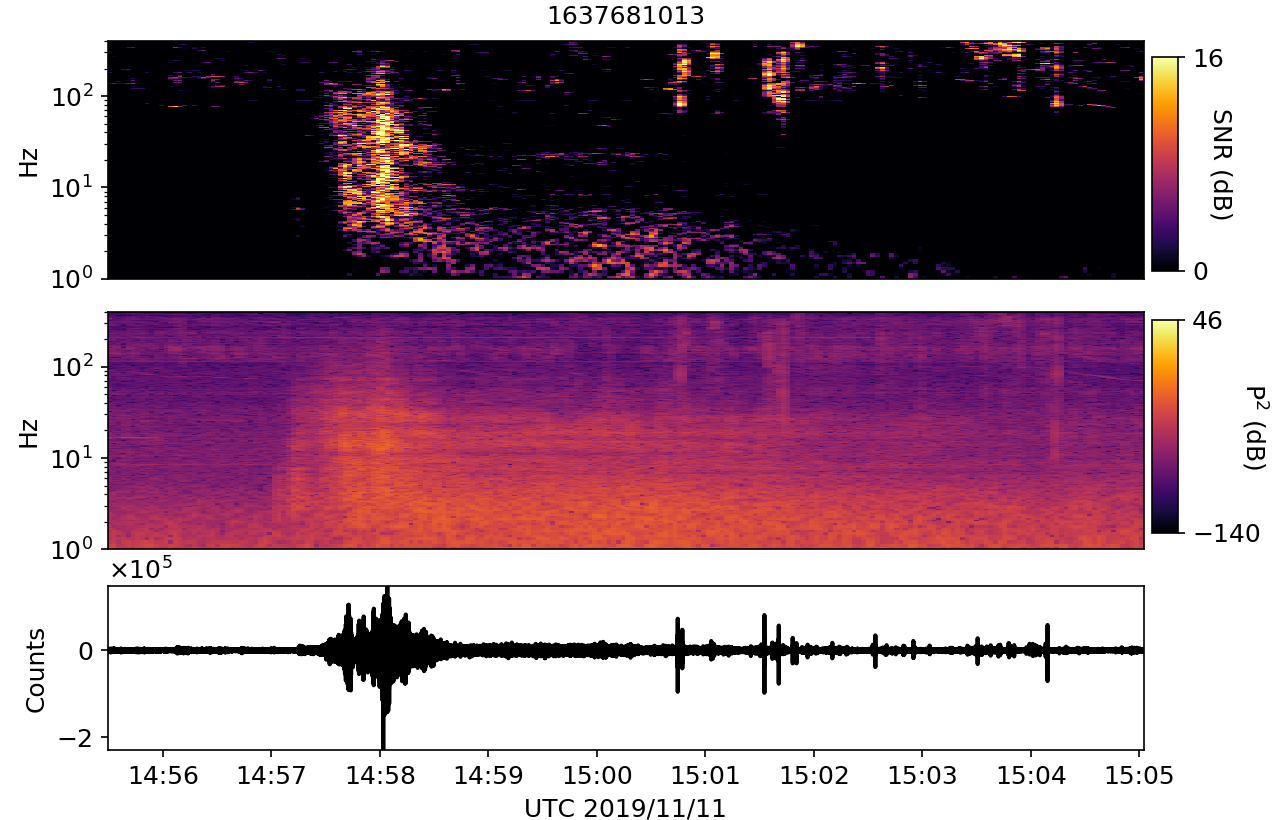
\includegraphics[width=\linewidth]{figures/spacex_1.png}
    \caption{Infrasound of Meteor Entry}
    \label{fig:spacex_1}
\end{figure}

The initial launch can be observed around 14:58 UTC with the stage 1 landing occurring near 15:02 UTC.

Figure~\ref{fig:spacex_2} shows the locations of the source and sensors for the SpaceX launch.

\begin{figure}[H]
    \centering
    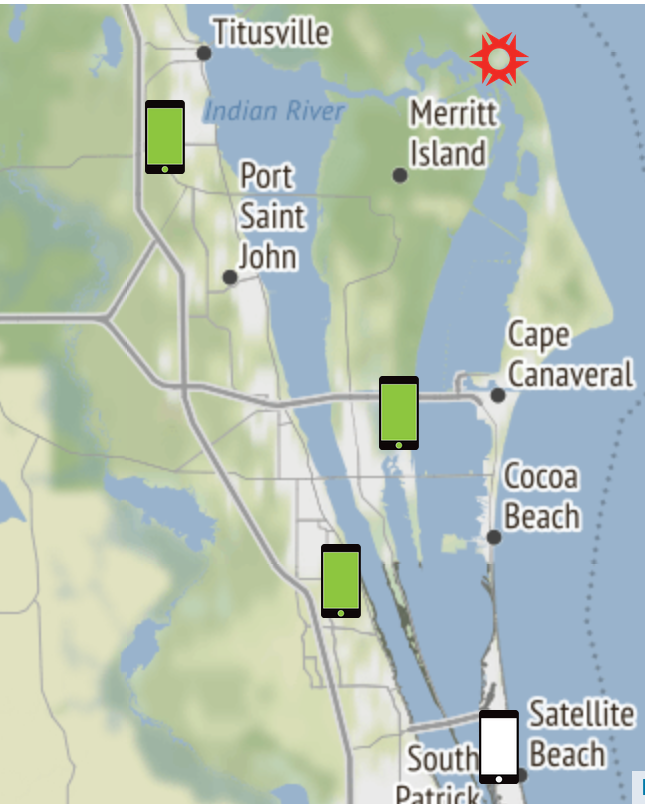
\includegraphics[width=.5\linewidth]{figures/spacex_2.png}
    \caption{Infrasound of Meteor Entry}
    \label{fig:spacex_2}
\end{figure}

\subsubsection{Hurricane Lane}

Hurricane Lane was a major hurricane that passed close to the Hawaiian islands on August 24, 2018\cite{wiki:Hurricane_Lane}. The Lokahi network observed the passing of the storm using its barometer sensors (which is still considered to be in the infrasound range) with 12 sensors stationed on Oahu and the Big Island.

Figure~\ref{fig:hurricane_1} displays the barometer readings over a 24 hour window showing the storm's arrival and departure in the infrasound range.

\begin{figure}[H]
    \centering
    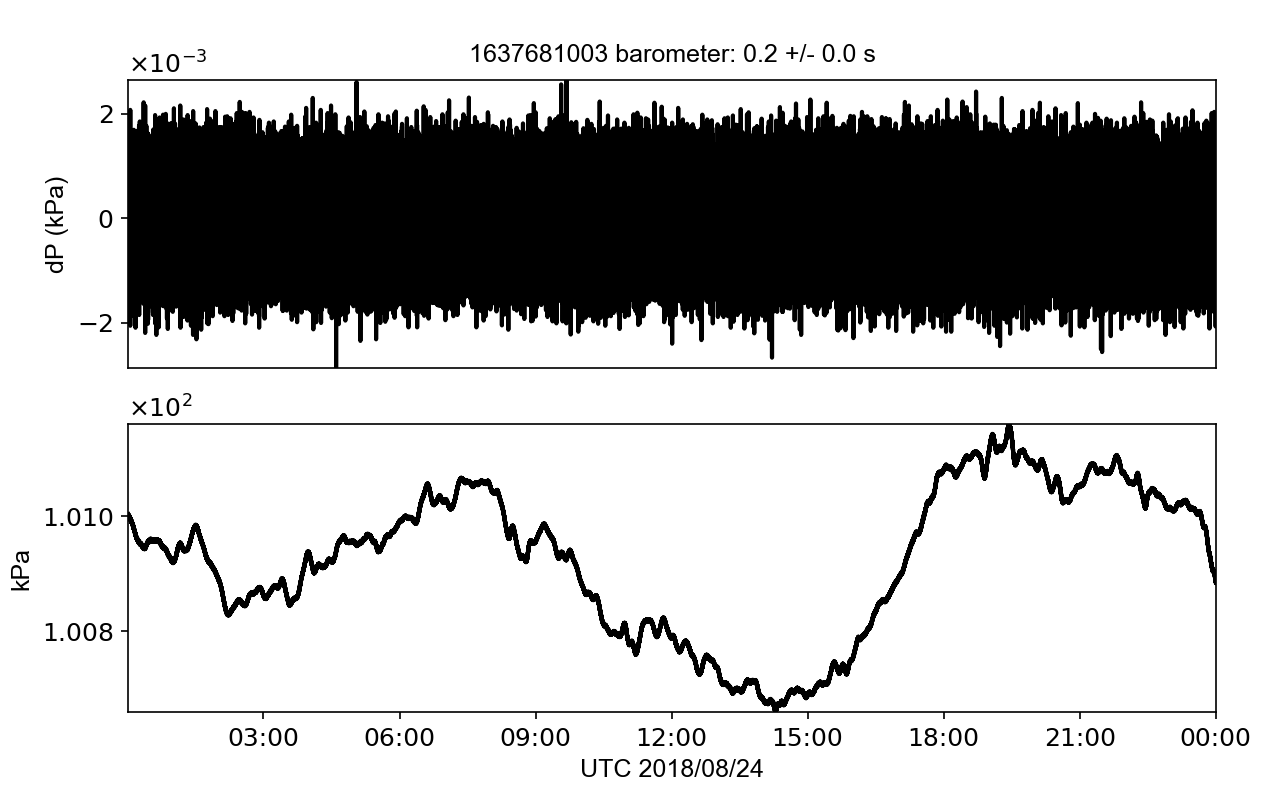
\includegraphics[width=\linewidth]{figures/hurricane_1.png}
    \caption{Barometer Readings of Hurricane Lane}
    \label{fig:hurricane_1}
\end{figure}

I've provided evidence that Lokahi is able to characterize infrasound signals over a wide variety of source modalities including infrasound caused by ground movement, storms, rocket launches, and atmospheric entries.

\subsubsection{Availability of Lokahi}

One of Lokahi's goals is to ensure data delivery in the face of network outages. Lokahi achieves this by buffering recorded data on board the mobile sensors until a time that a network becomes available. Luckily, most Lokahi based sensors are mobile phones which provide gigabytes of storage space. Depending on the sensor, it is possible to store weeks worth of data when a network is absent or restricted.

Lokahi only stores metrics on data received and does not know if a sensor is trying to send data, but is not able to. Because of this restriction, I setup a controlled experiment with 5 Lokahi based sensors. Over the course of the week, I disabled network access on the sensors for periods of 1 minute, 1 hour, 4 hours, and 1 day. I confirmed that the network outage data was missing and then re-enabled network access. I then confirmed that 100\% of originally missing data was uploaded to the Lokahi servers.

At least in a controlled environment, Lokahi was able to restore 100\% of its data. Anecdotally, we've observed issues in other deployments where networks have been spotty rather than either fully present or fully not present. We've encountered small amounts of data loss (on the order of minutes) in such situations. It is possible to suffer data loss in situations with incredibly spotty networks, but in my experience, this is quite rare.

\subsubsection{Other Claims Supporting the Generality of the Lokahi Network}\label{subsec:other-claims-supporting-the-generality-of-the-lokahi-network}

I've showcased a multitude of signals that the Lokahi framework has generated, but I believe there are other tangibles to consider.

The Lokahi network supported the Hawaiian Volcano Observatory during the 2018 lower Puna eruption by supplementing scientists with infrasound data produced by venting gases from magma chambers.

The Lokahi network directly supports several national laboratories (Idaho National Labs, Lawrence Livermore National Labs, Oakridge National Labs, and Lawrence Berkeley National Labs) by providing a secure channel to share real time infrasound data from strategically placed sensors. This data is consumed by the national labs and then analyzed and fused with other data streams in an effort to support the Labs' missions. The research group responsible for working with the Lokahi network works directly with the national labs providing guidance and support on the data.

The Lokahi network also supports several private groups by providing secure real-time data collected from strategically placed sensors.

Finally, the Lokahi network has served as the basis for several students to receive their graduate degrees. Julie Schnurr received her Masters degree in 2017 for her thesis ``Air Blasts: Explosion Yield Estimation and Waveform Modeling"\cite{julie} using data in part collected by Lokahi. Karina Asmar received her Ph.D\cite{asmar19} in 2019 using data collected by the Lokahi network.

\subsection{Discussion on Types of DSNs Laha is Suitable For}\label{subsec:discussion-on-types-of-dsns-laha-is-suitable-for}

In the Introduction Sections~\ref{subsec:anticipated-contributions} and~\ref{sec:anticipated-contributions-of-laha}, I stated that I would provide a discussion on the types of DSNs that Laha is suitable for. Working with two different DSNs in two different domains has provided me the opportunity to think about Laha's strengths and weaknesses compared to the domain that it is being utilized in. It's also given me the opportunity to think about other domains that Laha would be useful for. I will first discuss the strengths and weaknesses as compared to OPQ and Lokahi directly.

I find Laha's data savings in the lower levels of the Laha hierarchy to be useful in situations where the sensors have high sampling rates and where the raw data will eventually be sent to the cloud for analysis. This is true of both OPQ and Lokahi who have sampling rates of 12,000 Hz and up to 8,000 Hz respectively. In both cases, the raw data is sent to the cloud for further analysis. In OPQ, this takes place when triggering algorithms detect an Event. In Lokahi, the raw data is sent along with the high level AML feature extracted data. When TTL is implemented for these networks, we observe a large decrease in stored data and an increase in stored signal-to-noise ratio.

Networks with low sampling rates (on the order of seconds to minutes and higher) would not see as large of benefit in terms of storage savings due to the low sampling rate. In fact, networks with low sampling rates may benefit from a store everything approach if the resources are available.

Laha's data savings at higher levels in the hierarchy are only achievable for long running networks. Further, Laha's self-optimization capabilities only kick in over longer durations of network uptime. Because of this, Laha is better suited for networks with longer lasting deployments. Laha would be too cumbersome and not provide enough benefits for short lived, ad-hoc networks.

Laha is incredibly well suited for networks that experience a low signal to noise ratio. When most of the data is noise, Laha's data management combined with its ability to filter out noise in analysis puts it in a unique position to deal with large volumes of noisy data. Networks with a high signal-to-noise ratio would not gain the data saving benefits that Laha provides.

Laha attempts to classify Events and Incidents in near real time. If Events and Incidents are not classified in a timely manner, the underlying data might be garbage collected. Because of this, Laha is suited for networks that send data features in a timely manner. Sensors within the Laha framework are expected to be networked. Laha is ill suited for networks that don't provide data in a timely manner such as those that require physical access to get the data or those that buffer the data for long durations before transmitting. Further, Laha expects all data to arrive at a central location for further processing. This requires a network where each sensor in the network is able to send its data to an analysis process. Laha is not suited for networks where data must be retrieved from each sensor.

One of the major differences between OPQ and Lokahi is the number of identified Events and Incidents. Events and Incidents for OPQ are automatically found and classified and as it turns out, there is a lot going on on the UHM micro-grid in terms of PQ signals of interest. Contrast this to Lokahi which aims to classify significant signals observed in the infrasound range. Because the thresholds are higher for classifying Lokahi Events and Incidents, there are naturally less of them. This dichotomy is important because higher levels of the Laha hierarchy make use of large numbers of Events and Incidents to produce viable Phenomena. Because of that, Laha is better suited for networks that produce large amounts of Events and Incidents. These larges amounts of Events and Incidents provide Laha a greater opportunity to produce Phenomena and self-tune.

An interesting consequence of the above is that data at different levels in the two networks appear to provide different weights of importance. For example, Events and Incidents are somewhat rare in the Lokahi network due to the high threshold required to become an Event or Incident. These Incidents are generally infrasonic events that are well characterized. Because of the high threshold and rarity of these data types, the Incidents that are classified by Lokahi tend to provide greater context than Events and Incidents in OPQ where there are many more Events and Incidents and I rely on Phenomena to find important signals of interest. This leads me to believe that networks with large amounts of Events and Incidents are better analyzed with Phenomena where networks with low amounts of Events and Incidents may not necessarily need Phenomena to provide use context and actionable insights.

Networks that require only binary classifications or a small number of classifications would not be well suited by Laha. As an example, a network of temperature sensors that only creates Events when a threshold is crossed is likely better served by edge processing or sending all the data and only saving high level metrics and thresholds event indications. Laha really shines when it has the ability to apply multiple classification to multimodal data and to act on those classifications with Phenomena.

Networks that only send high level metrics (e.g. AML values) would be a difficult fit for Laha as Laha relies on the fact that it can access high-fidelity data to perform analysis in the Detection and Incident levels. Laha can still be used (from the AML up), but I suspect the quality of the results to greatly suffer.

I found that it's much easier to build a Laha network from the ground up compared to integrating Laha into an existing network. OPQ was designed with the explicit purpose of being a Laha compatible network. Further, OPQ, being an academic project, had the freedom to allow me to make any changes required to fit the implementation to the theory.

Lokahi on the other hand has goals of providing a secure and stable Infrasound network. Lokahi also provides much of the basis for work done at the Infrasound Laboratory in Kailua-Kona and at other institutions by our collaborators. Because of these requirements, it was more difficult to make sweeping changes specifically to fit Laha's model.

I believe that Laha would be useful in many distributed sensing domains that collect large amounts of data and provide opportunities for many different types of signal classifications. Although not part of my direct research, Lokahi is experimenting with including other sensor data other than infrasound such as magnetometer, accelerometer, gyroscope, light, and barometer in order to provide more sensing modalities. Laha provides a basis for integrating and analyzing these new sensing modalities.

In summary, I believe Laha would be a great fit for long running networks that provide high data rates and multiple classification possibilities. These include networks that perform earth quake monitoring, environmental monitoring, traffic monitoring, and security monitoring to name a few. As network speeds increase and as the availability  Laha is not well suited for networks with low data rates or simple classifications schemes.

\subsection{Discussion of Laha Levels}\label{subsec:discussion-of-laha-levels}

In the Introduction Sections~\ref{subsec:anticipated-contributions} and~\ref{sec:anticipated-contributions-of-laha}, I stated that I would provide a discussion on Laha hierarchy. Now that I've had the chance to implement Laha levels in two separate DSNs, I want to discuss my thoughts on the layout of the levels and the individual levels themselves.

To summarize, Laha utilizes 5 levels. The Instantaneous Measurements Level (IML) includes sampled raw data waveforms. The Aggregate Measurements Level (AML) contains summary statistics about features extracted from the IML. The Detection Level (DL) utilizes Events to define windows of data that may or may not contain signals of interest. The Incident Level (IL) contains data and metadata for classified signals of interest. The Phenomena Level (PL) provides context to groupings of subsets of data and also provides the ability to predict Future signals of interest all the while providing optimizations for the rest of the levels below it.

I believe that these original levels worked well in both DSN domains that I analyzed, however, there are a few things that would be interesting to experiment with in future work.

The IML is a bit contrived for some networks. Take OPQ as an example. The IML solely exists on the OPQ Boxes themselves bounded by the available memory. This is in contrast to all other levels which co-exist within a single cloud infrastructure. It feels like the IML is a bit removed from the rest of the levels because of this.

When Events are found, the IML data is copied into the Event. Similarly, IML data is copied into Incidents. This is in contrast to all other levels which do not perform any copying and merely ``point" to the data. For example, Incidents and Events simply point to a range of Measurements and Trends instead of copying those values into those levels. This is possible because the TTL values of those Measurements and Trends match those of the Events, Incidents, or Phenomena.

I think it would be useful to add another level under the IML called the Sensor Measurement Level (SML). This level would signify all of the raw data that is currently living on the sensors themselves and hasn't been sent to a central server for analysis. I would keep the IML, but this level would contain all of the raw samples that were sent from sensors to a central server. Instead of copying data into Events and Incidents, the data would remain in the IML and simply be referenced from Events and Incidents.

I believe the AML is critical and I'm not sure that I would make any changes to it directly. It alone is responsible for providing the triggering architecture required for detecting Events. However, I would consider adding a new level between the AML and the DL called the Data Fusion Level (DFL).

The DFL would be responsible for collecting AML data from heterogeneous sources. For instance, I found myself wishing that I had a way to feed ground truth data into OPQ alongside the OPQ Box data in an attempt to perform real time validation of our data. It would also be interesting to fuse other data sources such as temperature data, weather data, or power usage data in an attempt to find correlations between other data streams and what was observed by the OPQ Boxes. I would place the DFL between the AML and DL because I would like the DL an IL to be abstracted over AML values.

In certain instances, I believe the DL and IL could be combined into a single level. The main difference between Events and Incidents is that Incidents provide a known classification and only reference a subset of the Event data. It would be easy to combine these levels into a single Detection Level that has parameters listing known classifications within the Event along with timestamps. This would require less housekeeping and potential data savings by not copying the Incident waveform from the Event waveform.

I would not make many changes to the PL. I believe the PL is fundamentally important for providing context for large amounts of Events and Incidents.

I think there is room to create sub-levels within the main levels. For example, sub-levels could be added to perform compression, encryption, metric collection, quality assurance, or logging. These are currently handled by individual Actors within the levels, but in certain instances, I think it could be helpful to promote these ideas to sub-levels as useful parts of the Laha hierarchy.

\section{Results of Converting Primitive Data into Actionable Insights}\label{sec:results-of-converting-primitie-data-into-actional-insights}

Converting primitive data into actionable insights in one of the main tenants of this framework as described in Section~\ref{subsec:ability-to-convert-primitive-data-into-actional-insights}. This is accomplished within Laha by moving data upwards through Laha's hierarchy. Results for converting primitive data into actionable insights were found using the guidelines provided in the Evaluation Section~\ref{subsec:evaluation-of-converting-primitive-data-into-actionable-insights}.

Within Laha, raw sampled signals (IML) are first converted into low fidelity feature streams (AML). This provides context by extracting known features from the signal and providing a summary statistics view of those features. Within OPQ, raw ADC samples are converted to feature streams that contain minimum, maximum, and average values for Voltage, Frequency and THD. Within Lokahi, raw ADC samples are converted to feature streams that include summary statistics about the sampled data as well as a summary statistics for other fields (such as location and timing accuracy). In, both networks, raw samples are converted to feature streams which add context to the original data. These feature streams provide actionable insights in the form of informing higher levels in the hierarchy if a nominal signal is likely within that stream. This brings us to the Detections Level (DL).

The DL is responsible for identifying Detections which provide a window that includes metadata, IML, and AML data which may or may not include signals of interest. Detections add context to the AML in the form of metadata (such as window length and sensors affected). Detections are found either manually (in the case of Lokahi) or using a triggering algorithms (OPQ). Detections provide actionable insights by providing the Incidents Level (IL) with the chance to classify known signals of interest from the Detection window. Without Detections, Incidents could not be found as easily. Once a Detection has been observed, the data is forwarded to the IL where signal classification occurs.

The IL is responsible for classifying signals of interest against known signals. Multiple Incidents can be found within a single detection. The IL provides added context in the form of these classifications. These classifications are actionable because they inform us about anomalous conditions on the network. These conditions are useful for others who might want to further investigate why anomalous signals were observed. For example, if many Voltage sags are observed by OPQ for a single device, it alerts others that there may be a power issue somewhere in the building that the sensor is located. This issue may or may not need to be addressed, but it is actionable.

Perhaps the most interesting actionable insights Laha gathered are from Phenomena.

\subsection{Results of Phenomena}\label{subsec:results-of-phenomena}

When I first conceptualized Phenomena, I expected them to be useful for providing context to data that didn't exist at lower levels. Being able to determine if a signal is periodic or not is interesting. Being able to decide if Incidents are similar is interesting. Being able to create Future/Predictive Phenomena is interesting. All of these Phenomena are interesting in their own right, but I believe the greater discovery is that Phenomena provide a way to filter out the signal from the noise. They provide a way of grouping lots of similar signals together so that they can be discussed as a group. This is something that all Phenomena have in common, they take collections of signals found at lower levels which have been grouped in such a way that they can be discussed as a grouping of data.

The design of Phenomena can be found in Section~\ref{sec:phenomena} with implementation details outlined in Section~\ref{ssec:pq_plugins}. Evaluation guidelines can be found in Sections~\ref{subsec:evaluation-of-converting-primitive-data-into-actionable-insights} and~\ref{sec:evaluation-of-tertiary-goals}.

\subsubsection{Results of Annotation Phenomena}

Annotation Phenomena provide the means to add context to groupings of Events, Incidents, and sensors as mentioned in Section~\ref{subsec:annotations-phenomena}). Annotations contain a description grouping together related data as well as meta-data further describing the related data. Annotations add context on top of general classifications. As an example, Incidents within OPQ only provide information related to the PQ classification that it was assigned. However, this tells us nothing more about how the Incidents might be related (or if they even are related) and tells us nothing about the source of the anomalous signals.

Because Incidents within the Lokahi network require human vetting before publishing, all Incidents are assigned Annotations on Incident creation. These Annotations include a description of the signal source and also provide meta-data for linking the signals to known publications. For example, in previous sections, I showed that Lokahi was able to detect a meteor entry into the Earth's atmosphere above the Hawaiian islands. The Annotation for this Incident provides information about the source as well as provides links to third-party sources that verify the signal of interest. The Lokahi network contains 41 Annotations. Each Annotation in the Lokahi network groups one or more sensors that observed the same Incident.

The OPQ network has far fewer Annotation Phenomena. The reason for this is that I do not know the source for many of the PQ signals observed by the OPQ network. Only a small handful of PQ signals have a known source. These known source signals became the Annotation Phenomena in the OPQ network. Table~\ref{table:annotation_summary} summarizes the Annotation Phenomena observed by OPQ.

\begin{table}[H]
    \centering
    \caption{Summary of Annotation Phenomena}
    \begin{tabularx}{\textwidth}{lllll}
        \toprule
        \textbf{Description} & \textbf{Time (UTC)} & \textbf{Boxes} & \textbf{Events} & \textbf{Incidents}  \\
        \midrule
        Oahu Storm & 2019-10-11 00:00 & 16 & 4 & 400 \\
        Makiki Power Outage & 2019-10-16 22:37 & 16 & 1 & 143 \\
        Manoa Power Outage & 2019-11-23 20:02 & 15 & 1 & 168 \\
        \bottomrule
    \end{tabularx}
    \label{table:annotation_summary}
\end{table}

Annotation Phenomena within OPQ has allowed me to provide context and groupings for a total of 6 Events and 711 Incidents that otherwise would just be ``just another Event or Incident" and are now ``Events and Incidents caused by storms and power outages".

Annotations not only provide extra context on top of groupings of data, but they also affect the data that is stored. If an Annotation is created early enough, all Measurements, Trends, Events, and Incidents related to the Annotation will have their TTL values updated to be the same as the Annotation Phenomena. The end result is that the data that is grouped by the Annotation is saved for as long as the Annotation, allowing further analysis and saving data that has been contextualized. This is true of all Phenomena discussed in this section.

At this stage, Annotation Phenomena provide a way to discuss related Events, Incidents, and sensors. In networks that have large amounts of Events and Incidents, this can be a valuable tool to assign context to related data and help filter the signal from the noise. Annotations are essentially fancy labels with some metadata to describe the data. This would be useful for any future work that intends to add machine learning to the Laha framework.

I admit that Annotation Phenomena is representationally simple, however, I believe it adds great value in terms of contextualizing a large amount of Events and Incidents and for providing actionable insights that are useful to the consumers or this data. As an example, it's much more informative to say ``Lokahi observed a rocket launch" than it is to say ``Lokahi observed a non-nominal spike in the infrasound range". In a similar vain, it's much more informative to say ``OPQ observed Voltage sags relating to a power outage in Manoa" than it is to say ``OPQ observed Voltage sags across multiple sensors".

I would like to integrate Annotation Phenomena with other Phenomena such as Periodic or Similarity Phenomena. However, a lack of known signal sources for OPQ and a lack of Incidents for Lokahi make this difficult. Annotation Phenomena are most useful when an observed signal has a known source or when there are a large amount of Annotations in conjunction with a large amount of Events and Incidents. Future work should examine how to better integrate Annotation Phenomena with other Phenomena in an attempt to provide automatic Annotation classifications.

\subsubsection{Results of Periodic Phenomena}

Periodic Phenomena identify periodic signals of interest as described in Section~\ref{subsec:periodicity-phenomena}. Mauka has identified four periodic Phenomena. Table~\ref{table:periodic_summary} summarizes the results of observed Periodic Phenomena.

\begin{table}[H]
    \centering
    \caption{Summary of Periodic Phenomena}
    \begin{tabularx}{\textwidth}{Xlllllll}
        \toprule
        \textbf{Box} & \textbf{Period} & \textbf{Std} & \textbf{Peaks} & \textbf{Periods} & \textbf{Events} & \textbf{Incidents} & \textbf{Mean Deviation} \\
        \midrule
        1021 & 2127.55 & 8.81 & 41 & 463 & 332 & 4 & -3.14 \\
        1003 & 1406.75 & 81.66 & 17 & 263 & 11 & 4 & 1.03 \\
        1023 & 2017.0 & 60.21 & 5 & 298 & 47 & 0 & -1.25 \\
        2001 & 2760.0 & 123.75 & 5 & 236 & 0 & 0 & 1.61 \\
        \bottomrule
    \end{tabularx}
    \label{table:periodic_summary}
\end{table}

The major metrics utilized for evaluating the quality of periodic Phenomena are the number of peaks identified in the autocorrelated signal and the standard deviation of those peaks. A single peak or two peaks does not provide any information about if a signal if periodic or not. Two peaks could be periodic, but it could also just be a coincidence. Three peaks is the minimum amount of peaks that classify something as potentially periodic, however the confidence would be extremely low.

In the Table above, we see that Box 1021 has a periodic signal with 41 peaks, Box 1003 observed 17 peaks, and Boxes 1023 and 2001 only display 5 peaks. From this data, I'm only confident that Boxes 1021 and 1003 provide enough peaks to classify the data as truly periodic. Boxes 1023 and 2001 do not provide enough peaks to be confident enough that these are actually Periodic Phenomena.

It should be noted that Box 2001 is not part of the OPQ UH micro-grid deployment. This Box was sent to EPRI for evaluation purposes. Other than the summary provided above, I will leave Box 2001 from these results due to lack of ground truth data and due to the fact that this Box is not officially part of the deployment designed for this dissertation.

Because Box 1021 provides the best metrics in terms of both peaks and standard deviation, I will focus my results to that sensor.

Box 1021 in MSB experiences periodic Voltages sags as shown in the second panel of the Trend data presented in Figure~\ref{fig:v_perio}.

\begin{figure}[H]
    \centering
    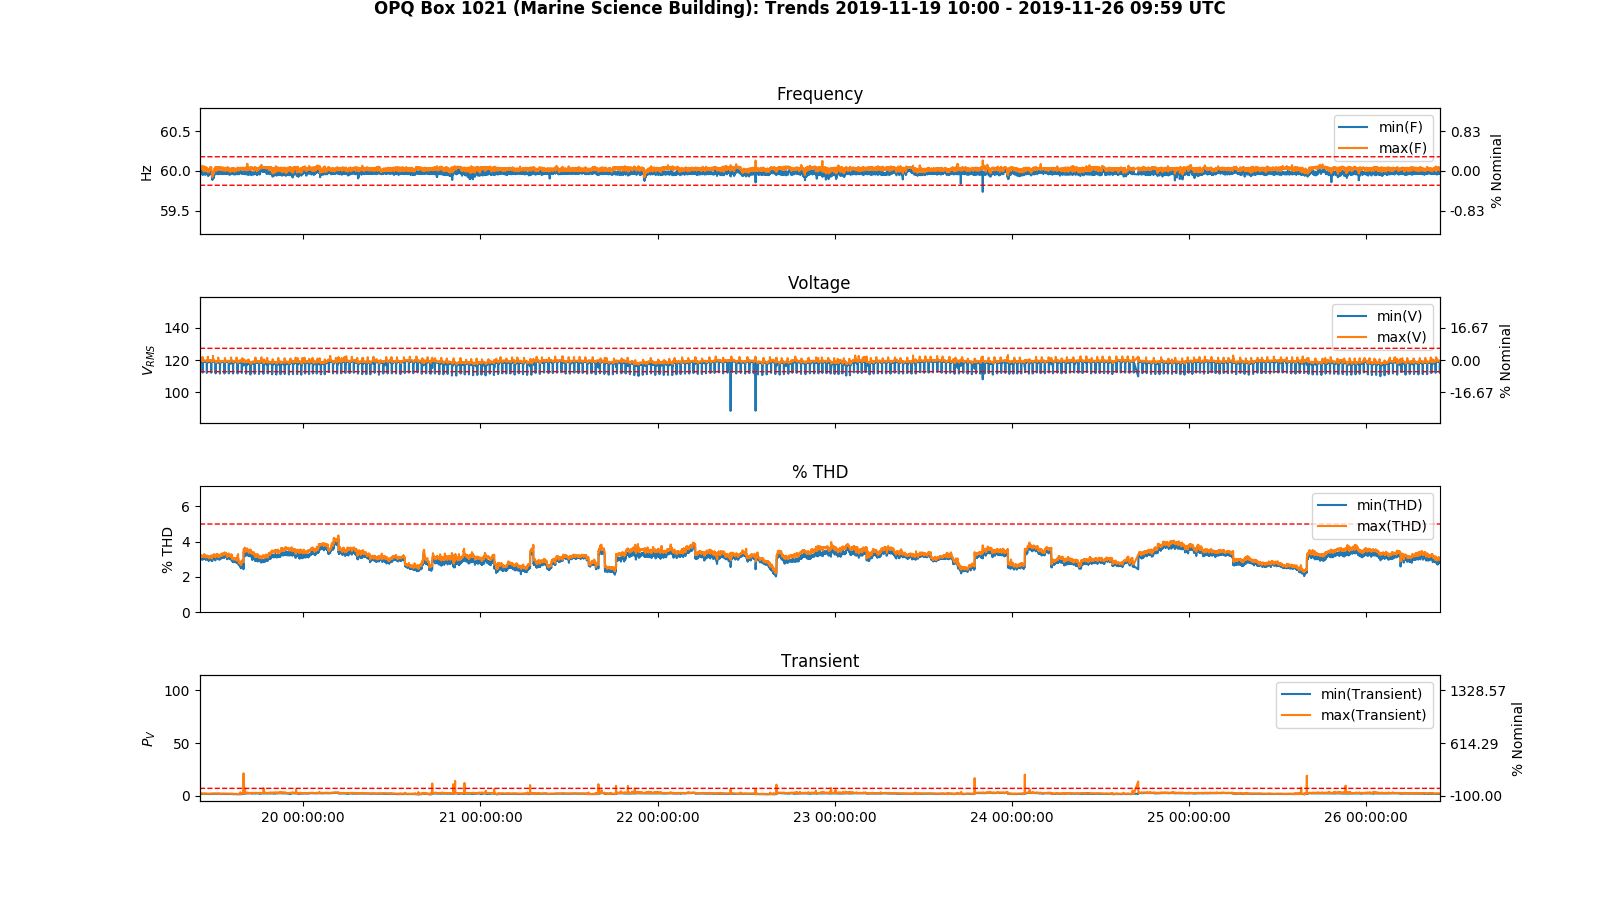
\includegraphics[width=\linewidth]{figures/v_perio.png}
    \caption{Periodic Voltage Sags}
    \label{fig:v_perio}
\end{figure}

The above figure shows many periodic Voltage sags over the course of one week. These Voltages sags have been present over the entire deployment of the OPQ network and were not observed by Boxes outside of MSB.

These Voltage sags were identified as periodic within Mauka's Periodicity Plugin. The original signal had its DC offset removed by subtracting the mean of the signal from the signal. Then the signal was filtered using a 4th order Butterworth high-pass filter. The filtered signal was then autocorrelated with itself. The distance between the peaks of the autocorrelation provide the period between peaks in the original signal. The mean of the peaks is the mean period of the Periodic signal. The Periodicity Plugin also finds the standard deviation of of the peaks found during autocorrelation. The combination of the mean period and the standard deviation of the period are then used to find the original times of the peaks and to produce Future Phenomena.

Once the plugin has a measure of mean period and standard deviation of the period, peak finding is employed to find the peaks of the original signal (as opposed to the autocorrelated signal). The peak finding algorithm is parameterized to not find peaks with a width less than that of the mean period minus the standard deviation of the period. These newly identified peaks provide timestamps and deviations from nominal for original periodic signal.

Figure~\ref{fig:periodic_example_2} shows an example of the Periodic Phenomena observed by Box 1021.

\begin{figure}[h]
    \centering
    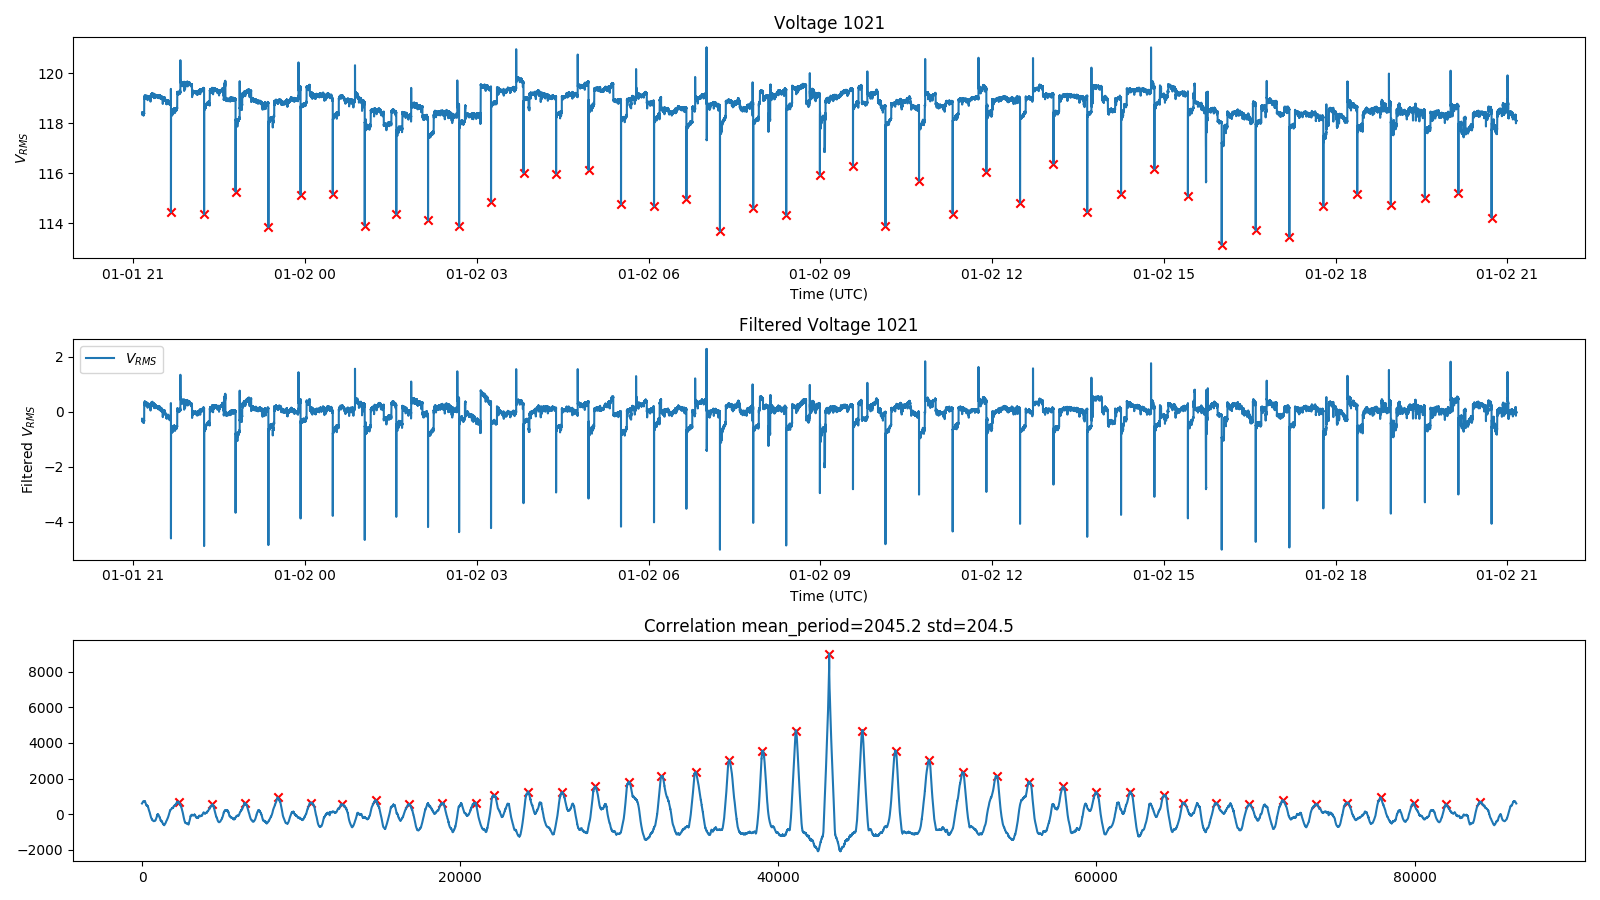
\includegraphics[width=\linewidth]{figures/periodic_example.png}
    \caption{Periodic Phenomena Example}
    \label{fig:periodic_example_2}
\end{figure}

The above figure shows the original signal in the top panel, the filtered signal in the middle panel, and the autocorrelated signal in the bottom panel. The mean and standard deviation of the autocorrelation peaks were used to identify the Voltage sag peaks in the original signal on the first panel. The timestamps and deviations from nominal are then extracted from the peaks in the first panel and stored in the database to be utilized by Future Phenomena.

Phenomena are designed to provide adaptive optimizations to the DSN. Periodic Phenomena provide optimizations in several ways. First, Periodic Phenomena get better over time. Because of the stability of the signal, consecutive runs of the Periodicity Plugin provide more accurate results during times when there is less noise in the periodic signal. Over time, the plugin is able to identify periodic signals with smaller standard deviations than previous runs. As the standard deviation becomes smaller, the accuracy of detecting periodic signals becomes higher.

As an example, when the periodic signal at Box 1021 was originally identified, the plugin identified a signal with a period of 44 minutes and a standard deviation of close to 9 minutes. Over the course of about a week, the Periodic Phenomena self optimized and now provides a period of about 35.5 minutes and a standard deviation on the order of 8 seconds. This matches what I observed empirically and in the ground truth data.

Periodic Phenomena self-optimizes by utilizing data gathered from Future Phenomena. Future Phenomena adjust the underlying Event thresholds and the Measurement and Trend rates of OPQ Boxes. During the time window of a future Phenomena, Measurement and Trend rates are increased while Event thresholds are decreased. The net result of this is the ability to detect Events that would not have otherwise been detected. More importantly, by increasing the Measurement rate, the periodicity plugin gains higher fidelity data from the increased data rate which in turn provides Periodic Phenomena the ability to better classify periodic signals of interest, thus decreasing the standard deviation and increasing the accuracy of the plugin. The Periodicity Plugin and Future Plugins work in conjunction to optimize each other. The more accurate the Periodic Phenomena become, the more accurate the Future Phenomena become and vice versa.

One of the tenants of Periodic Phenomena (or one of the tenants of Phenomena in general) is to identify groupings of Events and Incidents that occurred during the period identified by the Phenomena. The summary Table presented in the beginning of this section provides counts for the number of Events and the number of Incidents that correspond with periodic signals of interest. For example, OPQ Box 1021 identified a total of 463 periods that should have observed a Voltage drops. Of those 463 periods, 332 (or about 72\%) of the periods contained Events that were identified by Mauka. Four Voltage sag Incidents were also observed during these periods. This is to be expected as most of the Voltage sags observed by 1021 do cross the Event thresholds, but the deviation from nominal is not large enough to pass the Voltage Incident thresholds. This Phenomena provides groupings of Events and Incidents that are related to the periodic signal of the sensor. This is important because previously these were just Voltage sags Events and Voltage sag Incidents. This Phenomena adds context to these Events and Incidents by providing a grouping that shows that they were part of a periodic signal rather than individual PQ issues. The next section will show how Future Phenomena modifies Event thresholds in order to capture Events that might otherwise be missed due to not passing the Event thresholds.

I have attempted unsuccessfully to determine the cause of the periodic Voltage sags at this location. My original hypothesis was that the cycling of the building's HVAC units caused the Voltage sags. If that was the case, then it should be possible to see pressure changes in the infrasound range as the HVAC system cycled on and off. Going off of this assumption, I co-located a Lokahi sensor with the OPQ Box in MSB in an attempt to measure the HVAC cycles using the onboard barometer of the Lokahi sensor. After collecting data for one week, I was not able to observe any signals in the barometer data that correlated with the Voltages sags.

It is possible that the HVAC system is constantly pushing air through the building, but the coolant machinery kicks in once every 34 minutes. If this is the case, then the Lokahi sensor would not be able to identify changes in air pressure. One way to test this would be to install a temperature sensor on the OPQ Box to track changes in temperature. This would make for an interesting future direction allowing OPQ to track if changes in the environment are related to changes in PQ readings.

It should be noted that although Lokahi sensors record the temperature, they mainly record the internal temperature of the sensor's processor and these readings are generally not affected by the ambient temperature that the sensor resides in.

I've provided evidence in this section that show OPQ Mauka was able to identify Periodic Phenomena. I also showed how this Phenomena is able to provide optimizations to the DSN. I've shown the Periodic Phenomena is able to provide groupings for Events and Incidents, providing added context and actionable insights.

\subsubsection{Results of Future/Predictive Phenomena}

Future Phenomena are generated from Periodic Phenomena as described in Section~\ref{subsec:future-phenomena}. Future Phenomena predict when signals of interest should be observed by a particular sensor. Future Phenomena store information about its time window, the OPQ Boxes affected, and the expected feature that is predicted to be non-nominal. Future Phenomena also directly perform optimizations on the OPQ network. They are capable of modifying Event thresholds for the Frequency, Voltage, and THD features as well as modifying the data rate of OPQ Boxes. Because the Future Phenomena is capable of modifying the system, I expected to detect Events that would have otherwise been missed due to the threshold being too high.

The Periodic Phenomena that were discussed in the previous section play an important role in creating Future Phenomena. Future Phenomena are created based off of the mean period and standard deviation of the period from the Periodic Phenomena. Future Phenomena attempt to predict four hours of Events and Incidents from the last known timestamp of a Periodic Phenomena.

The value of four hours was chosen due the the interplay between the Periodicity plugin and Future Phenomena plugin. The Periodicity plugin runs once per hour and checks for periodic signals of interest using Measurements gathered over the previous 24 hours. Since I want the Future Phenomena to be optimized by Periodic Phenomena, I wanted to choose a value that was larger than one hour period used by the Periodicity plugin. I also didn't want to chose a large value for the similar reasons. The further out predictions are made, the less likely they are to be accurate. I expect the interplay between Future Phenomena and Periodic Phenomena to be such that predictions stay accurate due to the fact that the Phenomena optimize each other. By choosing a low number such a four hours instead of say twelve hours, a day or more, the system is more likely to make correct predictions.

Future work should investigate with changing these value or even creating multiple layers of predictions at different time scales to see how they affect the underlying system's ability to identify and predict periodic signals of interest.

Future Phenomena were generated from all four of the previous Periodic Phenomena discussed in the previous section. Table~\ref{table:future_summary} summarizes the results of Future Phenomena as implemented by OPQ Mauka.

\begin{table}[H]
    \centering
    \caption{Summary of Future Phenomena}
    \begin{tabularx}{\textwidth}{llll}
        \toprule
        \textbf{Box} & \textbf{Future Phenomena} &\textbf{Unrealized} & \textbf{Realized} \\
        \midrule
        1021 & 9 & 185 & 210 \\
        1003 & 113 & 52 & 61 \\
        1023 & 173 & 113 & 60 \\
        2001 & 91 & 91 & 0 \\
        \bottomrule
    \end{tabularx}
    \label{table:future_summary}
\end{table}

I use the term ``realized" to specify whether a Future Phenomena observed Events or Incidents. If a Future Phenomena does not contain any Events or Incidents, I use the term ``unrealized". The summary above shows that just over 53\% of all Future Phenomena for Box 1021 are realized. I had hoped that this value would be higher, but not all is lost. First, the amount of realized Events increases over time as the Future Phenomena self-optimize in conjunction with Periodic Phenomena.

Figure~\ref{fig:future_opt} shows the percentage of realized Future Phenomena over time.

\begin{figure}[h]
    \centering
    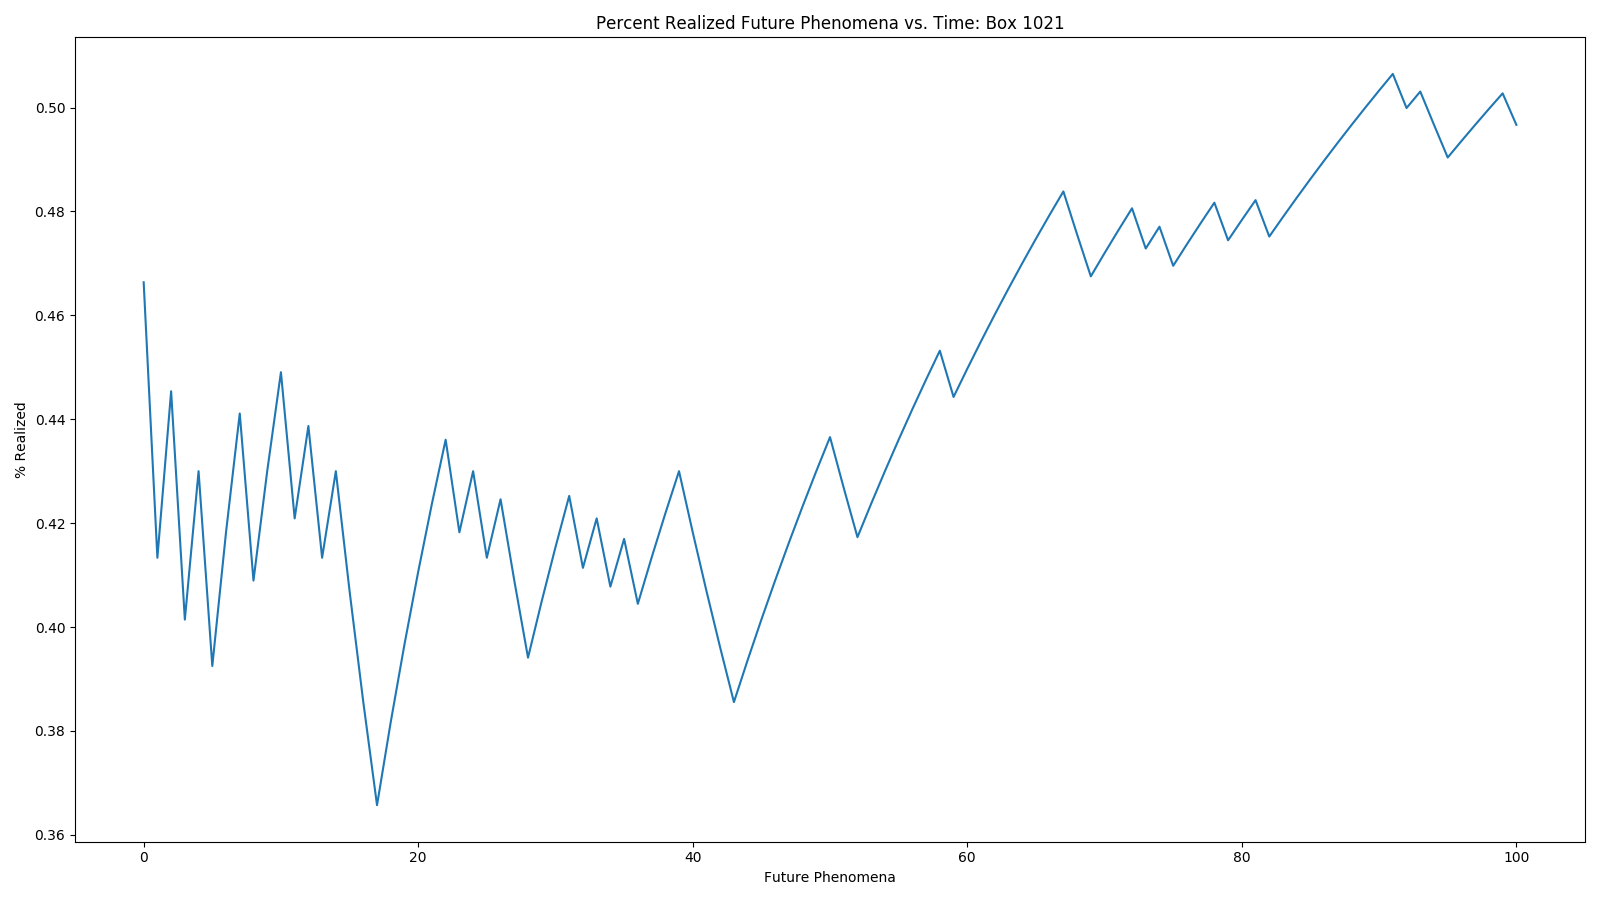
\includegraphics[width=\linewidth]{figures/future_opt.png}
    \caption{Future Phenomena Self-Optimization}
    \label{fig:future_opt}
\end{figure}

The Figure above shows that initially, the percentage of realized Events is fairly sporadic. Over time, as Future Phenomena and Periodic Phenomena apply optimizations to the underlying DSN, the amount of realized Future Phenomena increase.

Future Phenomena provide multiple optimizations to the underlying DSN. Future Phenomena can modify Event thresholds and data rates. These modifications increase data fidelity (which in turn helps to produce more accurate Periodic Phenomena), and also decrease Event thresholds. Because of the decreased Event thresholds, I expect Mauka to detect Events that would otherwise not have been detected.

Of the 210 realized Future Phenomena for Box 1021, exactly 37 of them contained sub-threshold Events, that is Voltage sag Events that are smaller than the default sag threshold of 2.5\% or 117.0 Volts. These 37 Events would not have been captured by the default Event trigger without modifications applied by Future Phenomena. Not only were these Events found using Future Phenomena, but they are also part of the Periodic Phenomena data set that created the Future Phenomena in the first place.

Figure~\ref{fig:sub_thresh_event} shows an example of a sub-threshold Event found utilizing Future Phenomena.

\begin{figure}[h]
    \centering
    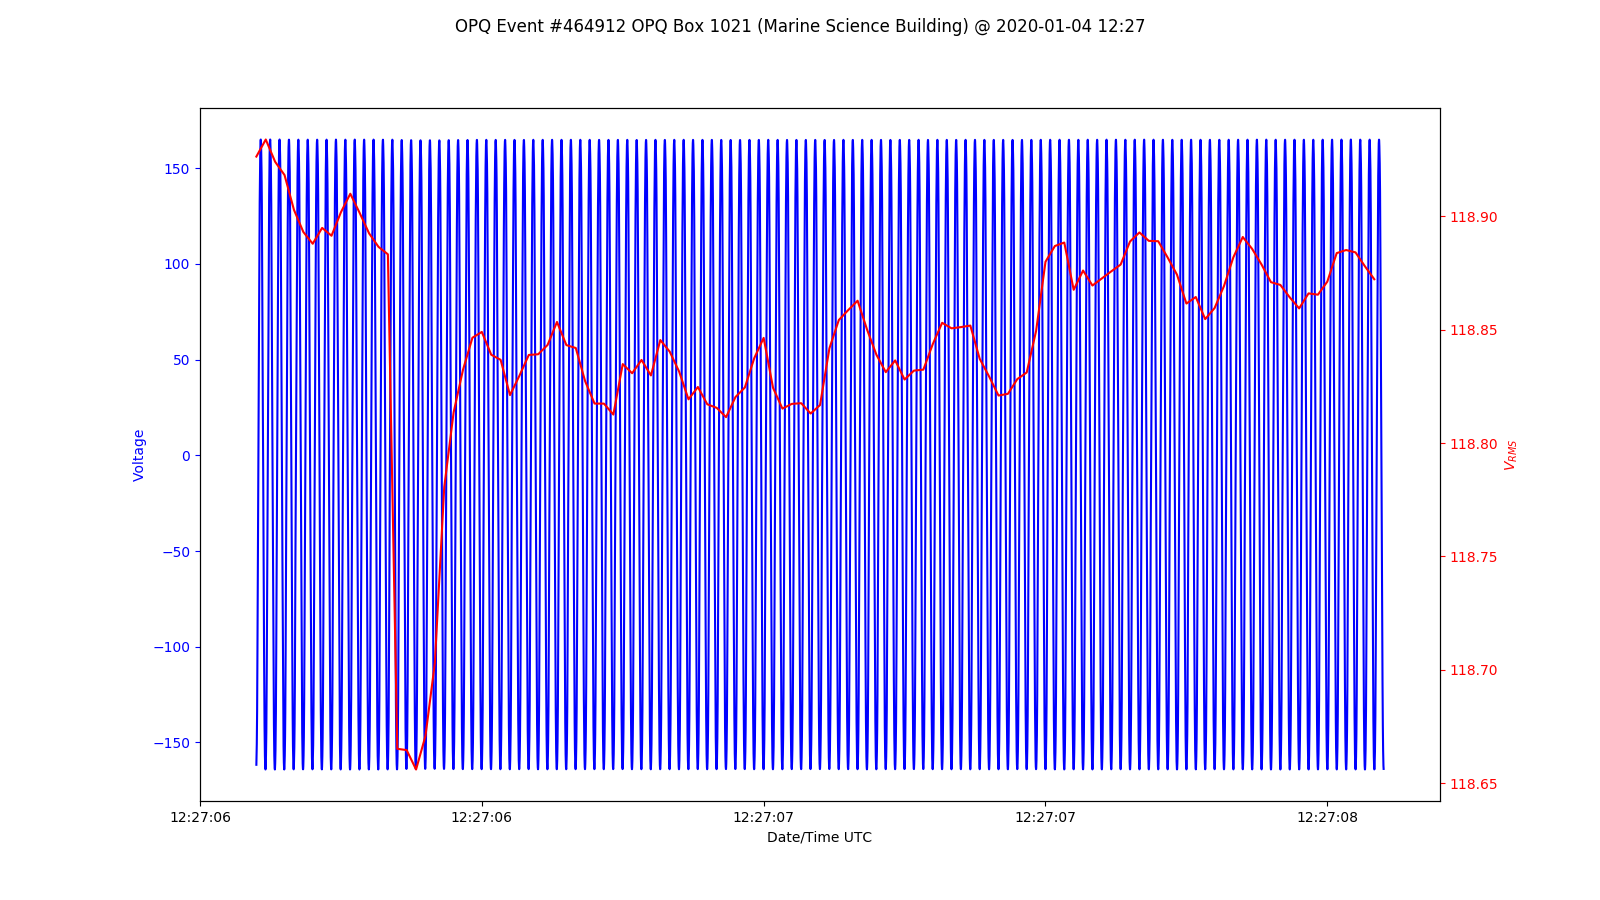
\includegraphics[width=\linewidth]{figures/event-single-464912.png}
    \caption{Sub-Threshold Event}
    \label{fig:sub_thresh_event}
\end{figure}

Here we can observe a Voltage sag of of just over 1\% deviation from nominal. This Voltage sag would not have been observed without modifying the Event thresholds using this Future Phenomena.

I have provided evidence that shows that the Future Phenomena are able to predict Future Events better than half of the time. I have shown that the Future Phenomena are capable of improving over time based off of optimizations applied by the Periodic Phenomena and Future Phenomena. I have shown that Future Phenomena are capable of detecting sub-threshold Events that would have otherwise been missed by normal triggering algorithms.

\subsubsection{Results of Similarity Phenomena}

% TODO
TODO

\subsubsection{Summary of Results for Converting Raw Data into Actionable Insights}

I've shown in previous sections that data for both the OPQ and Lokahi networks utilize the Laha hierarchy and that primitive data is indeed converted into actionable insights at higher levels within the hierarchy. I've shown how raw ADC samples are converted from level to level and provided discussion on what types of actionable insights can be gathered from each level within the Laha hierarchy.

I've shown that Phenomena add context to groups of Events and Incidents and that they are able to provide optimizations to the DSN which in turn increases the accuracy of the Phenomena.

\section{Results of Tiered Management of Big Data}\label{sec:dsn-system-requirements}

In the Introduction~\ref{subsec:tiered-big-data-management}, I provided tired management of big data as one of the major claims of Laha. In the Evaluation chapter~\ref{subsec:eval-big-data}, I examined the theoretical bounds of DSN system requirements both with TTL (Section~\ref{sssec:evaluation_of_ttl}) and without TTL (Section~\ref{sssec:eval_of_dsn_system_requirements}) for the OPQ and Lokahi networks.

This section will focus on examining the actual DSN system requirements for the OPQ and Lokahi networks.

All results in this section were gathered directly from the OPQ and Lokahi networks and no estimated parameters or simulations were used.

\subsection{DSN System Requirements: OPQ}\label{subsec:dsn-system-requirements:-opq}

System utilization metrics were collected during the deployment of the OPQ DSN. The metrics that were collected are provided in the description of the SystemStatsPlugin (Section~\ref{lbl:SystemStatsPlugin}). In summary, I collected metrics on plugin utilization, system resource utilization, garbage collection, tunable Laha parameters, and storage requirements for each level within the Laha hierarchy. Evaluations for these results are provided in Sections~\ref{sssec:eval_of_dsn_system_requirements} and~\ref{sssec:evaluation_of_ttl}.

There were several schema changes to the stored metric data, with the most significant change taking place on September 20, 2019. For these results, I only used metrics collected after this date as they contain the most useful data. Because of this, all actual data measurements have an offset that is greater than zero. That is, there was already data stored at each level before I started collecting detailed metrics. This offset is removed from the actual data when comparing to the theoretical data bounds in order to provide a more accurate comparison between the series.

Further, the astute reader will notice that there are often times more than 15 Boxes in the metric data when only 15 Boxes were deployed for the UHM deployment. This is attributed to the fact that several Boxes were sent to the Electric Power Research Institute (EPRI) to evaluate if our Boxes could be used as a test bed for their power quality analysis needs. The metrics collected by Laha are collected for the total set of all Boxes sending to OPQ, and thus, also sometimes include metrics from the Boxes that EPRI are evaluating.

First I will examine the storage requirements at each level within the hierarchy. I performed a linear regression on the total size at each level which can server as yet another measure for estimating the size of the OPQ network. Once the actual storage requirements have been examined in detail, I will compare the actual results to the theoretical results founds in previous sections.

\subsubsection{DSN System Requirements OPQ: IML}

The Instantaneous Measurements Level (IML) contains a window of raw samples from sensors. In the case of OPQ, these consist of the samples of data stored in the main memory of each OPQ Box. The IML has a TTL of 15 minutes which is determined by the available storage capacity of each OPQ Box.

The IML is unique in that data from the IML is never ``saved" by higher levels in the hierarchy. Instead, IML data is copied into Detections, Incidents, and Phenomena. Because of this, the size of the IML over time is function of the number of OPQ Boxes sending data at any particular time. Figure~\ref{fig:actual_iml_opq} shows the actual OPQ IML data growth over the deployment period. As can be observed, the IML size is a simple function of the number of OPQ Boxes sending data.

\begin{figure}[H]
    \centering
    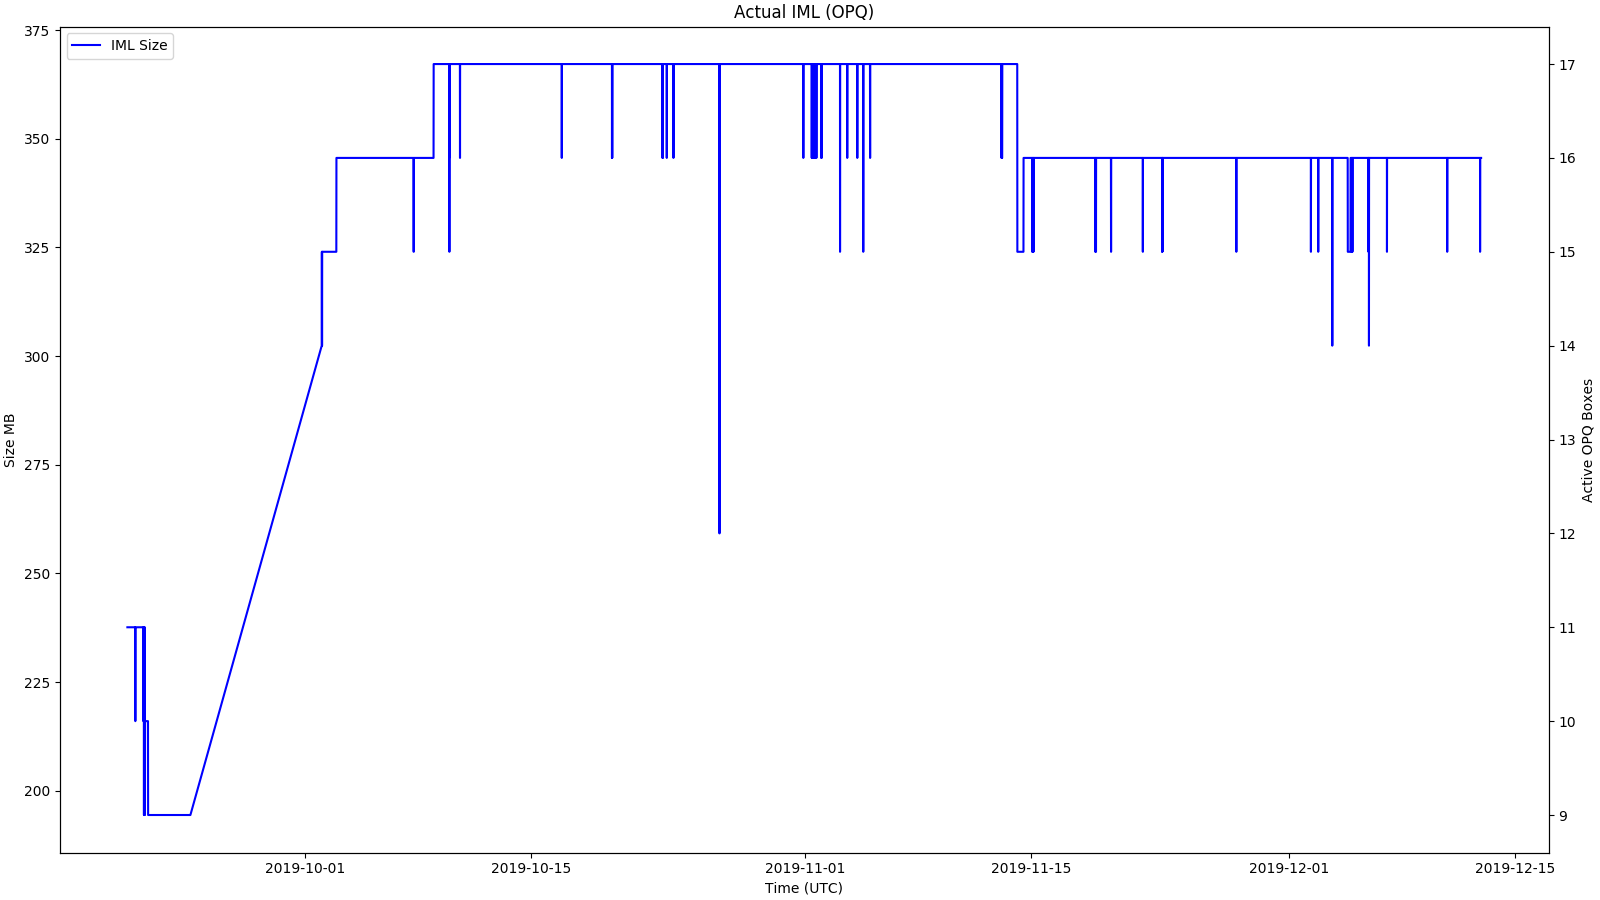
\includegraphics[width=\linewidth]{figures/actual_iml_opq.png}
    \caption{Actual IML for OPQ}
    \label{fig:actual_iml_opq}
\end{figure}

A deployment of 15 OPQ Boxes will consume about 325 MB of IML space. The changes in data size are attributed to the fact that OPQ Boxes came on and offline during the period of the OPQ deployment. At the lowest point, only 9 OPQ Boxes were sending and at the highest point 17 OPQ Boxes were sending data. Garbage collection doesn't take place in the traditional sense in the cloud at this level as the IML samples are stored on the OPQ Boxes and bounded by the available memory that each Box can store. This plot assumes that at each Box is storing 15 minutes worth of data in a circular buffer. The spikes in IML size are from data gaps in sensor data. Either the sensor was powered off or there were network connectivity issues.

I will compare this result to the theoretical results in following sections.

\subsubsection{DSN System Requirements OPQ: AML}

The Aggregate Measurements Level (AML) contains summary statistics of features extracted from the IML. OPQ contains two sub-levels within the AML (Measurements and Trends). Data within the AML can be saved by higher levels within Laha (DL, IL, and PL). If AML data is saved, it receives the TTL of the highest level that the data was saved by.

I examine the AML data growth for OPQ by looking at the data growth of Measurements, Trends, and the total AML. Figure~\ref{fig:actual_aml_opq} displays the AML growth for the OPQ network as well as statistics about garbage collection.

\begin{figure}[H]
    \centering
    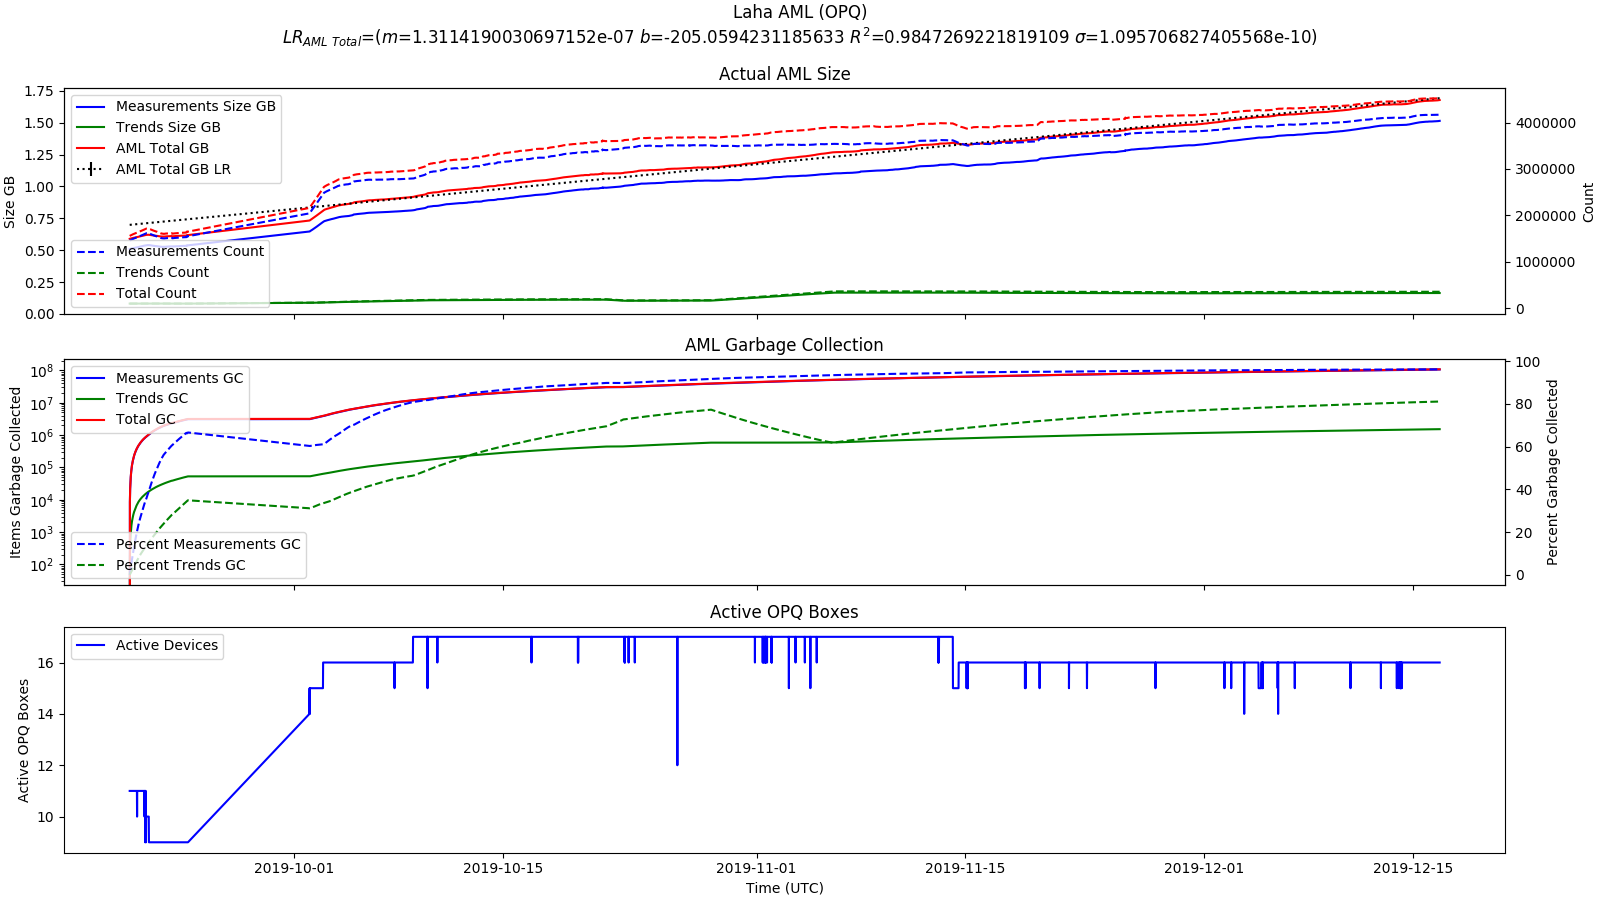
\includegraphics[width=\linewidth]{figures/actual_aml_opq.png}
    \caption{Actual AML for OPQ}
    \label{fig:actual_aml_opq}
\end{figure}

The top panel displays the AML data growth with size in GB on the left Y-axis and the count of AML items on the right Y-axis. Over a period of two and a half months the AML in OPQ has reached a size of about 1.75 GB containing over 4 million AML items.

The middle panel displays the number of Measurements and Trends that were garbage collected over time on the left Y-axis and the percentage of items that were garbage collected on the right Y-axis. About 98\% of all AML data was garbage collected. About 2\% of all AML data is either awaiting garbage collection or was ``saved" by a higher level in the Laha hierarchy.

The bottom panel displays the number of active OPQ Boxes over time. It's possible to see how the number of Boxes impacts the size of the AML. For example, the increase in Boxes in September and the decrease of Boxes in mid-November have noticeable impacts on the AML storage size.

Equation~\ref{eq:aml_si} provides the best fit linear regression for the total AML size in GB with an $R^2$ value = 0.98.

\begin{equation}
    y = 1.3114190030697152e-07 * x + 0.6987665459751351
    \label{eq:aml_si}
\end{equation}

This linear equation can be used to estimate the total AML data stored per OPQ Box over a given time period $x$. Simply substitute $x$ with the duration in seconds in the above equation, subtract the offset, and then divide by the mean number of active OPQ Boxes (15). Equation~\ref{eq:aml_si_ex} can be used to find the estimated AML size per OPQ Box over a duration of one month (28 days or 2419200 seconds) which is close to 0.3 GB per OPQ Box per month.

\begin{equation}
    y = \frac{(1.3114190030697152e-07 * 2419200 + 0.6987665459751351) - 0.58918365}{15}
    \label{eq:aml_si_ex}
\end{equation}

I will compare this result to the theoretical results in following sections.

\subsubsection{DSN System Requirements OPQ: DL}

The Detections Level (DL) contains metadata and data bounded by a time window that may or may not contain signals of interest. Detections are generated by threshold based triggering algorithms. Detections can be saved by higher levels in the Laha hierarchy (IL and PL) and will receive the same TTL as the highest level the DL data is saved by. The DL contains metadata about the window it examines, but the bulk of data is produced by the raw samples that get copied into the DL when a Detection is created.

Figure~\ref{fig:actual_dl_opq} shows the DL data growth for the OPQ network over time.

\begin{figure}[H]
    \centering
    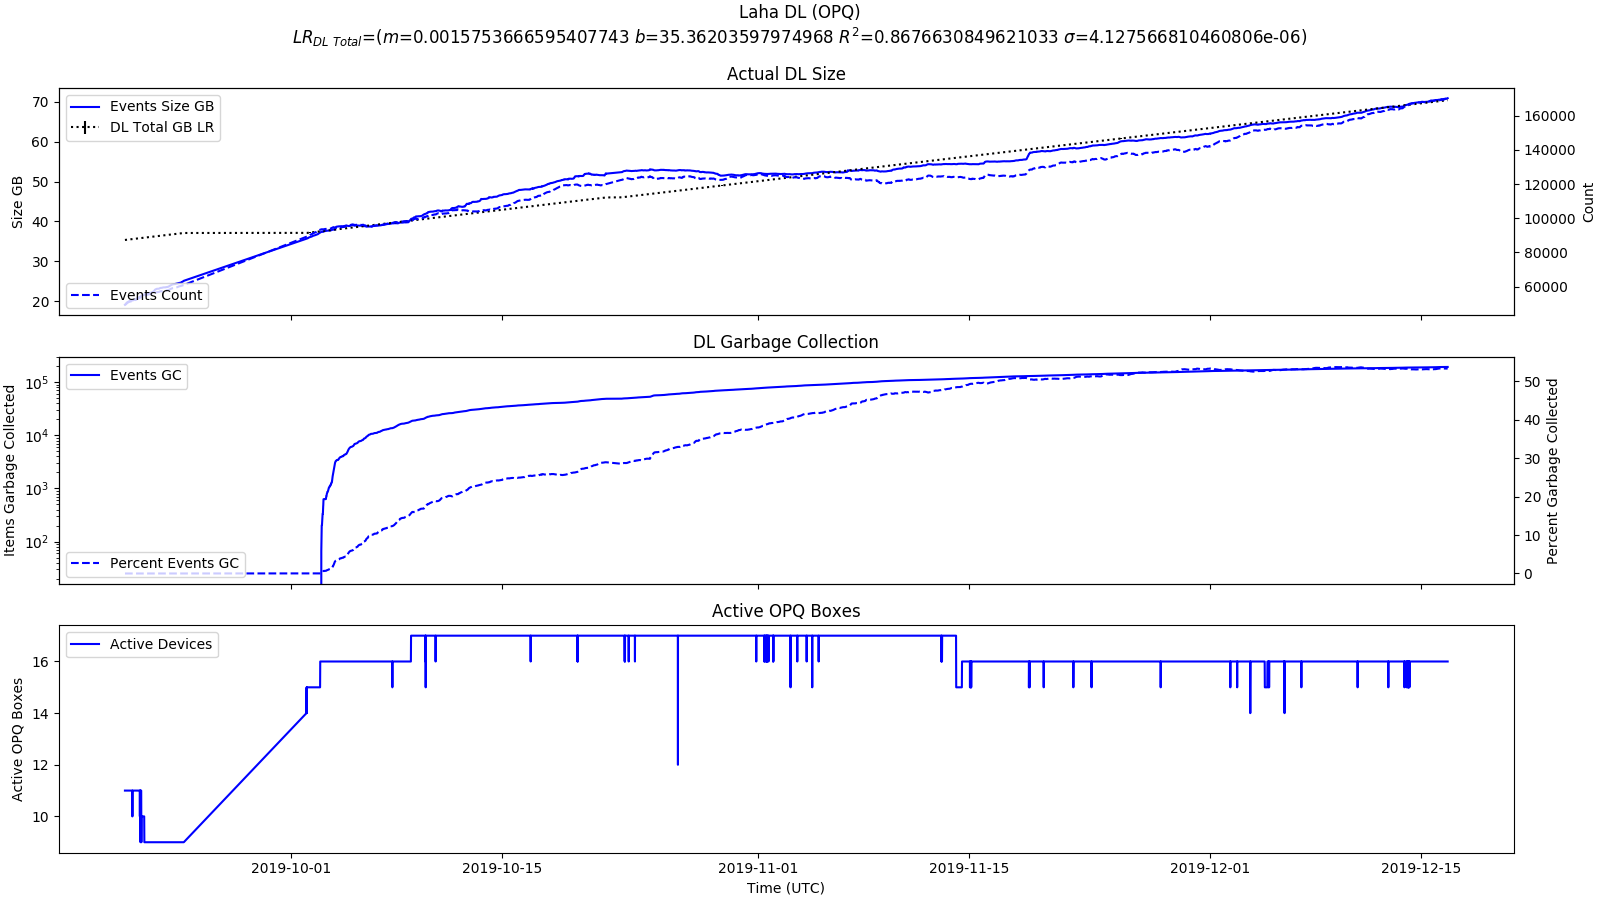
\includegraphics[width=\linewidth]{figures/actual_dl_opq.png}
    \caption{Actual DL for OPQ}
    \label{fig:actual_dl_opq}
\end{figure}

The top panel shows the size of the DL over time with the size in GB on the left Y-axis and the count of Detections on the right Y-axis. The size of the DL for the OPQ network has grown to close 70 GB over the period of two and half months containing a total of 160,000 Detections.

The middle panel shows the garbage collection statistics for the DL. Of note is the delayed uptick in garbage collection until October 1, 2019. This is a direct result of the fact that Detections have a TTL of 1 month, and thus, no Detections were garbage collected during the first month of data collection. As of two and a half months of data collection, about 50\% of all Detections generated have been garbage collected while the other 50\% are wither awaiting garbage collection or have been saved by Incidents or Phenomena.

The bottom panel shows the number of active OPQ Boxes sending data over time.

Equation~\ref{eq:dl_si} provides the best fit linear regression for the total DL size in GB with an $R^2$ value = 0.90.

\begin{equation}
    y = 5.0185766274104244e-06 * x + 32.21305865745437
    \label{eq:dl_si}
\end{equation}

This linear equation can be used to estimate the total DL data stored per OPQ Box over a given time period $x$. Simply substitute $x$ with the duration in seconds in the above equation, subtract the offset, and then divide by the mean number of active OPQ Boxes (15). Equation~\ref{eq:dl_si_ex} can be used to find the estimated DL size per OPQ Box over a duration of one month (28 days or 2419200 seconds) which is close to 1.68 GB per OPQ Box per month.

\begin{equation}
    y = \frac{(5.0185766274104244e-06 * 2419200 + 32.21305865745437) - 19.131860232}{15}
    \label{eq:dl_si_ex}
\end{equation}

I will compare this result to the theoretical results in following sections.

\subsubsection{DSN System Requirements OPQ: IL}

The Incidents Level (IL) contains metadata and data relating to classified signals of interest. Incidents are created when a Mauka plugin classifies a signal of interest from a Detection. Incidents can be saved by Phenomena.

Figure~\ref{fig:actual_il_opq} shows the IL growth for the OPQ network over a period of two and a half months.

\begin{figure}[H]
    \centering
    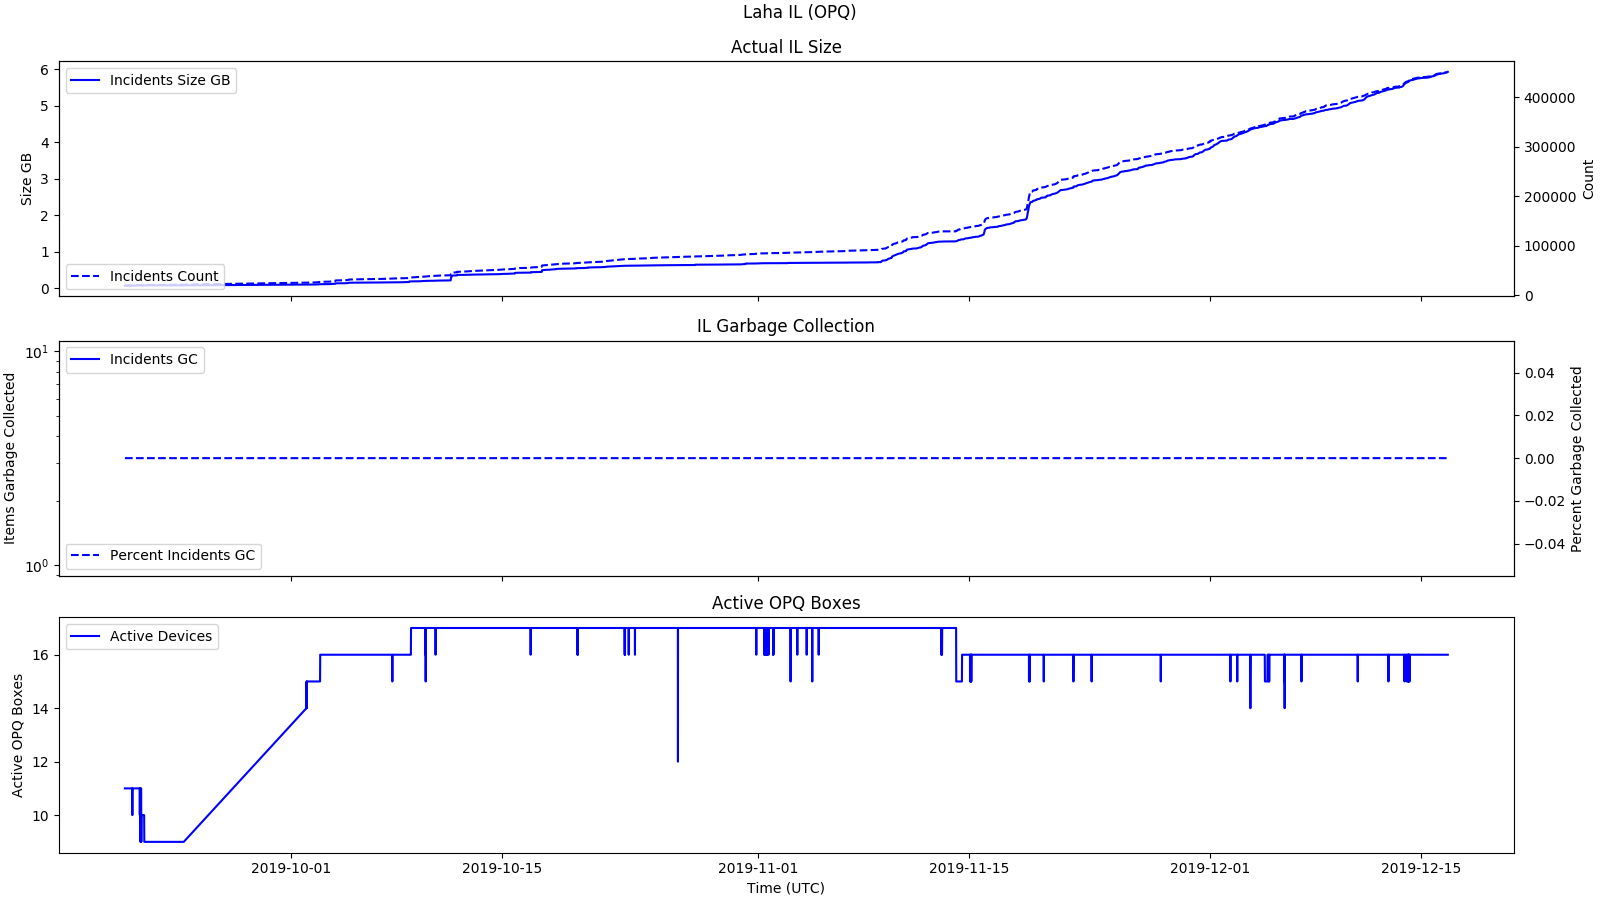
\includegraphics[width=\linewidth]{figures/actual_il_opq.png}
    \caption{Actual IL for OPQ}
    \label{fig:actual_il_opq}
\end{figure}

The top panel shows the growth of the IL with the size in GB on the left Y-axis and the number of Incidents on the right Y-axis. Over a period of two and a half months, the IL of OPQ has grown to near 6GB containing over 400,000 Incidents. The update in Incidents around mid-November is due to the fact that I performed maintenance on many of my Incident classification algorithms and also added a slew of Incident plugins. This also caused our linear regression fit to be the least accurate of any of the Laha levels.
The top panel shows the growth of the IL with the size in GB on the left Y-axis and the number of Incidents on the right Y-axis. Over a period of two and a half months, the IL of OPQ has grown to near 6GB containing over 400,000 Incidents. The update in Incidents around mid-November is due to the fact that I performed maintenance on many of my Incident classification algorithms and also added a slew of Incident plugins. This also caused our linear regression fit to be the least accurate of any of the Laha levels.

The middle panel shows the garbage collection statistics for the IL. You'll note that the GC statistics are flat lining at 0. This is due to the fact that Incidents are given a default TTL of 1 year and this deployment has only been collecting data for 3 months.

This brings up the question, is a TTL of 1 year for Incidents too long? It's clearly not useful over a deployment of 3 months, but DSNs utilizing Laha are expected to operate in a stable fashion for long durations. Incidents, only being one step below Phenomena, contain a wealth of information in the form of classified signals of interest. I believe that data that has been classified should live for a long time duration. Since Events live for a month and Phenomena live for a 2 years, it makes sense to me to have a TTL of 1 year for Incidents. One of the reasons I decided to simulate Laha in terms of data storage requirements was so that I could show expected results for time periods larger than that of the OPQ deployment. We could scale back the TTL of Incidents to 6 months, but this would still be beyond the range of the OPQ deployment duration. Future work on Laha will examine how altering TTLs of the various levels affect the underlying data storage characteristics.

The bottom panel shows the number of active OPQ Boxes sending data over time.

Equation~\ref{eq:il_si} provides the best fit linear regression for the total IL size in GB with an $R^2$ value = 0.83.

\begin{equation}
    y = 8.114350243481761e-07 * x + -1.4797678575319322
    \label{eq:il_si}
\end{equation}

This linear equation can be used to estimate the total IL data stored per OPQ Box over a given time period $x$. Simply substitute $x$ with the duration in seconds in the above equation, subtract the offset, and then divide by the mean number of active OPQ Boxes (15). Equation~\ref{eq:il_si_ex} can be used to find the estimated IL size per OPQ Box over a duration of one month (28 days or 2419200 seconds) which is close to 0.3 GB per OPQ Box per month.

\begin{equation}
    y = \frac{(8.114350243481761e-07 * 2419200 + -1.4797678575319322) - 0.072925535}{15}
    \label{eq:il_si_ex}
\end{equation}

I will compare this result to the theoretical results in following sections.

\subsubsection{DSN System Requirements OPQ: PL}

% TODO
TODO

\subsubsection{DSN System Requirements OPQ}

I will now examine the results of combining all Laha levels within OPQ. Figure~\ref{fig:actual_laha_opq} provides the results of data collection for the entire OPQ network over a period of 2 and a half months.

\begin{figure}[H]
    \centering
    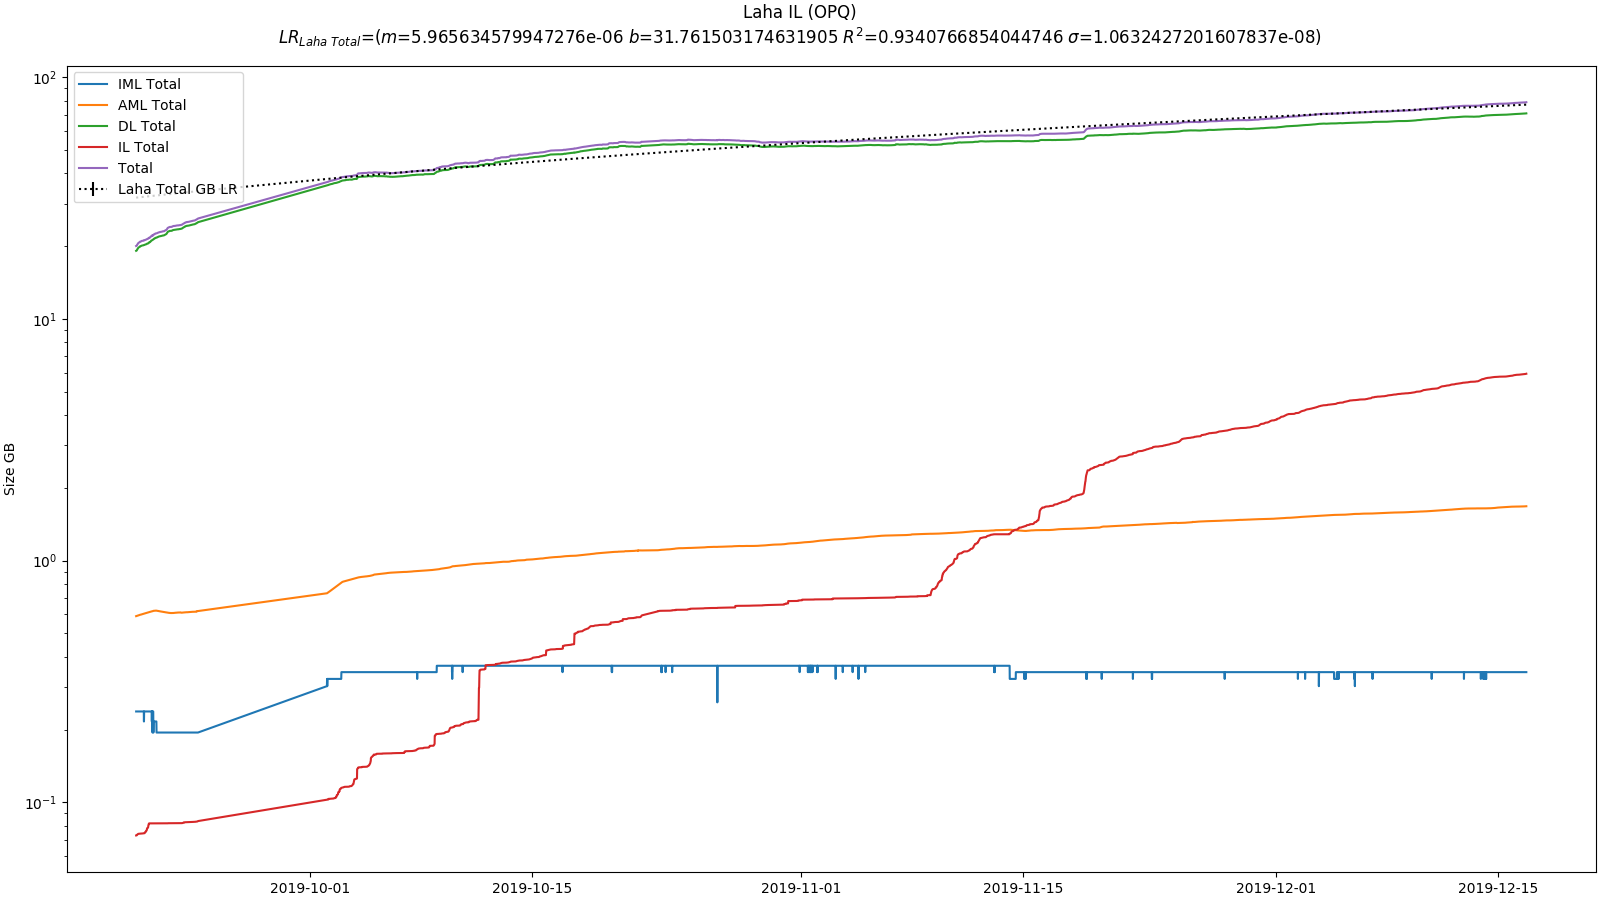
\includegraphics[width=\linewidth]{figures/actual_laha_opq.png}
    \caption{Actual Laha for OPQ}
    \label{fig:actual_laha_opq}
\end{figure}

First, please note that the Y-axis is using a log scale in order to better display the data growth of some of the smaller Laha levels. Next, we observe that the size of the entire network is just under 100 GB over a period of two and a half months with an average of 15 OPQ Boxes.

We can observe that the IML level converges to the smallest of the levels due to its strict 15 minute TTL.

The IL starts out small, but as Incidents are identified, the IL surpasses the IML at about 1 month and surpasses the AML in size at about 2 months. The Detections level is the largest and this makes sense since we treat Detections relatively cheaply and they contain windows of data that are generally larger than the signal of interest if there even is a signal of interest at all.

Equation~\ref{eq:laha_si} provides the best fit linear regression for the total Laha size in GB with an $R^2$ value = 0.93.

\begin{equation}
    y = 5.965634579947276e-06 * x + 31.761503174631905
    \label{eq:laha_si}
\end{equation}

This linear equation can be used to estimate the total Laha data stored per OPQ Box over a given time period $x$. Simply substitute $x$ with the duration in seconds in the above equation, subtract the offset, and then divide by the mean number of active OPQ Boxes (15). Equation~\ref{eq:laha_si_ex} can be used to find the estimated Laha size per OPQ Box over a duration of one month (28 days or 2419200 seconds) which is close to 1.74 GB per OPQ Box per month.

\begin{equation}
    y = \frac{(5.965634579947276e-06 * 2419200 + 31.761503174631905) - 20.031569417}{15}
    \label{eq:laha_si_ex}
\end{equation}

I will compare this result to the theoretical results in following sections.

\subsubsection{DSN System Requirements OPQ: Comparing Results to Estimates}

Now that I have shown the results for the actual DSN storage requirements, I will next compare these results to the estimated storage requirements with and without TTL\@.

Let us first compare the results to the estimated storage requirements without TTL found in Section~\ref{sssec:eval_of_dsn_system_requirements}. This might feel a bit contrived, but the purpose of these results is to show how OPQ compares to a similar system that would collect everything.

One interesting thing to note is that I expected the estimated values to be much higher than the actual values due to the fact that I was not including TTL explicitly anywhere in the estimations. It turns out this is not always the case. The reason for this is that the estimated values are computed by multiplying the amount of time the system has been running with the data rate obtained from the OPQ database for Events, Incidents, and Phenomena, and on the surface, it does not appear that TTL is being used in these estimations. However, this is not exactly the case. The data rate parameters obtained from the OPQ database implicitly have the TTL built in. That is because I measure the data rate over all available Events, Incidents, and Phenomena, but this data rate does not include Incidents, Events, or Phenomena that have been garbage collected! Unfortunately, I do not have detailed metrics on data that was garbage collected (only counts). Any future DSN utilizing Laha should consider recording detailed metrics about data that was garbage collected (duration, data stored, etc).

This really only affects Detections, Incidents, and Phenomena which use estimated database parameters. Samples, Measurements, and Trends are not affected because they are computed directly from the time length without using any estimated database parameters.

The end result of this is that it turns out that the method I use to estimate Events, Incidents, and Phenomena without TTL pretty accurately portray the size of the actual data with TTL.

There was already data in the database before we started collected enhanced metrics. This is true for the AML, DL, IL, and PL. In order to accurately compare data growths from zero, the first value at each level is subtracted from the entire data set at each level. This essentially ``forces" the data set to start at 0 so that we can compare it directly to the estimates.

\paragraph{IML Versus Estimated Growth}
The Instantaneous Measurements Level (IML) consists of raw samples from sensors. Figure~\ref{fig:actual_iml_vs_unbounded_opq} shows the actual IML vs unbounded IML\@.

\begin{figure}[H]
    \centering
    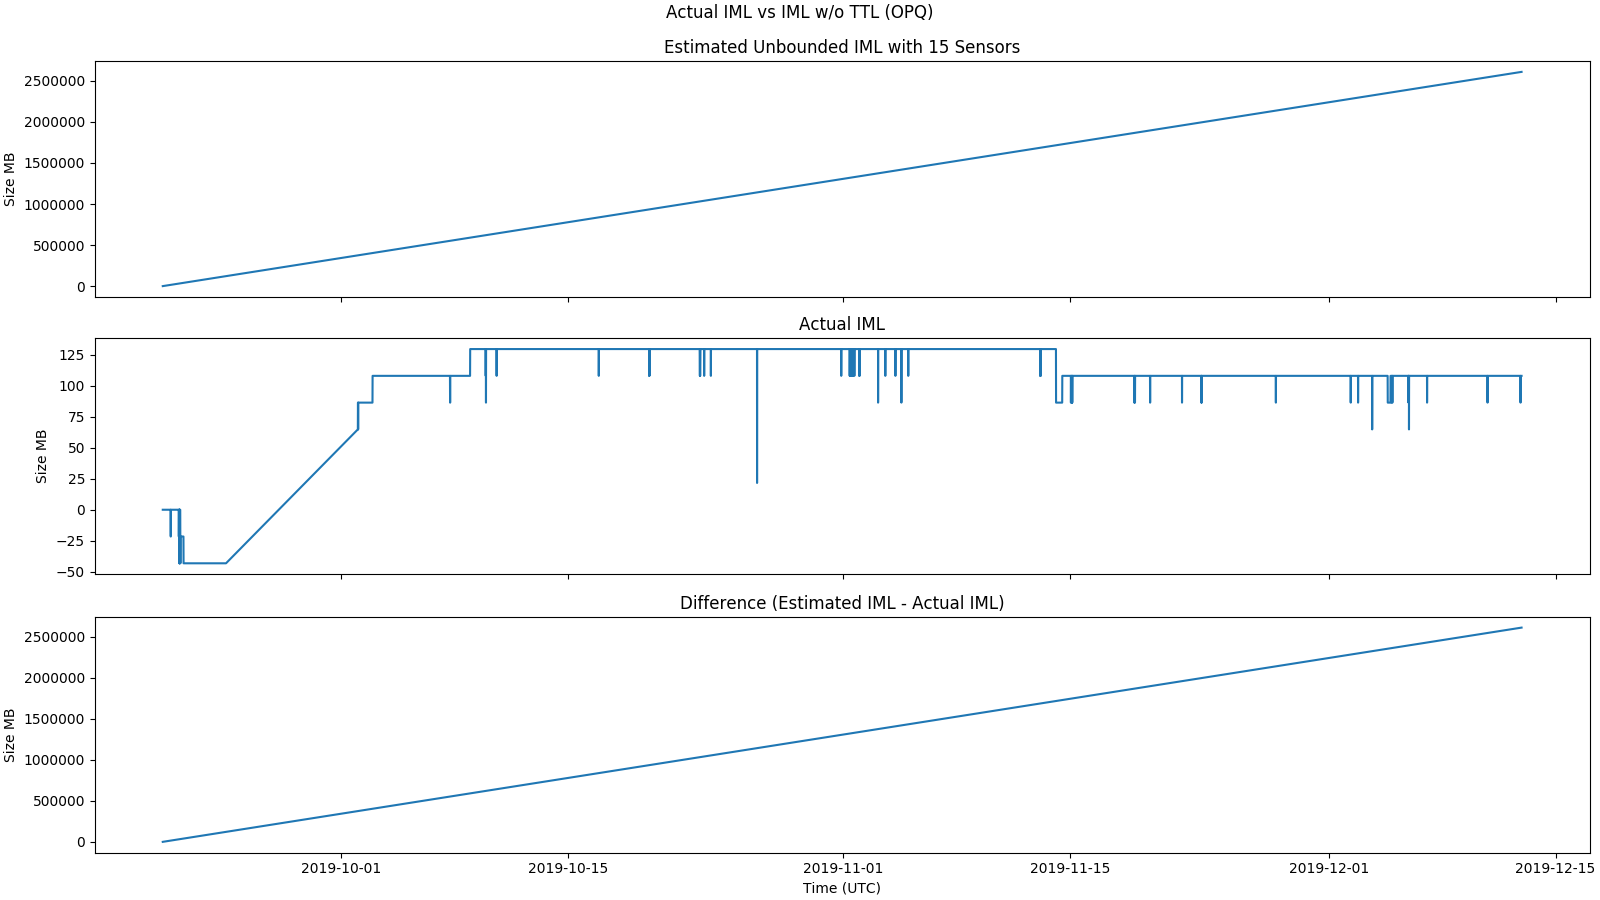
\includegraphics[width=\linewidth]{figures/actual_iml_vs_unbounded_opq.png}
    \caption{Actual IML vs Unbounded IML for OPQ}
    \label{fig:actual_iml_vs_unbounded_opq}
\end{figure}

This plot is a little uninteresting. The difference is lost by the shear imbalance between magnitudes. With the IML producing the most data consisting of raw samples, without a TTL of 15 minutes the unbounded IML grows very quickly. By having bounds on the data, OPQ saves over 2.5 TB worth of data storage.

\paragraph{AML Versus Estimated Growth}
Figure~\ref{fig:actual_aml_vs_unbounded_opq} shows the actual AML vs unbounded AML. The AML level contains aggregate measurements which are rolled up summary statistics extracted from the IML\@.

\begin{figure}[H]
    \centering
    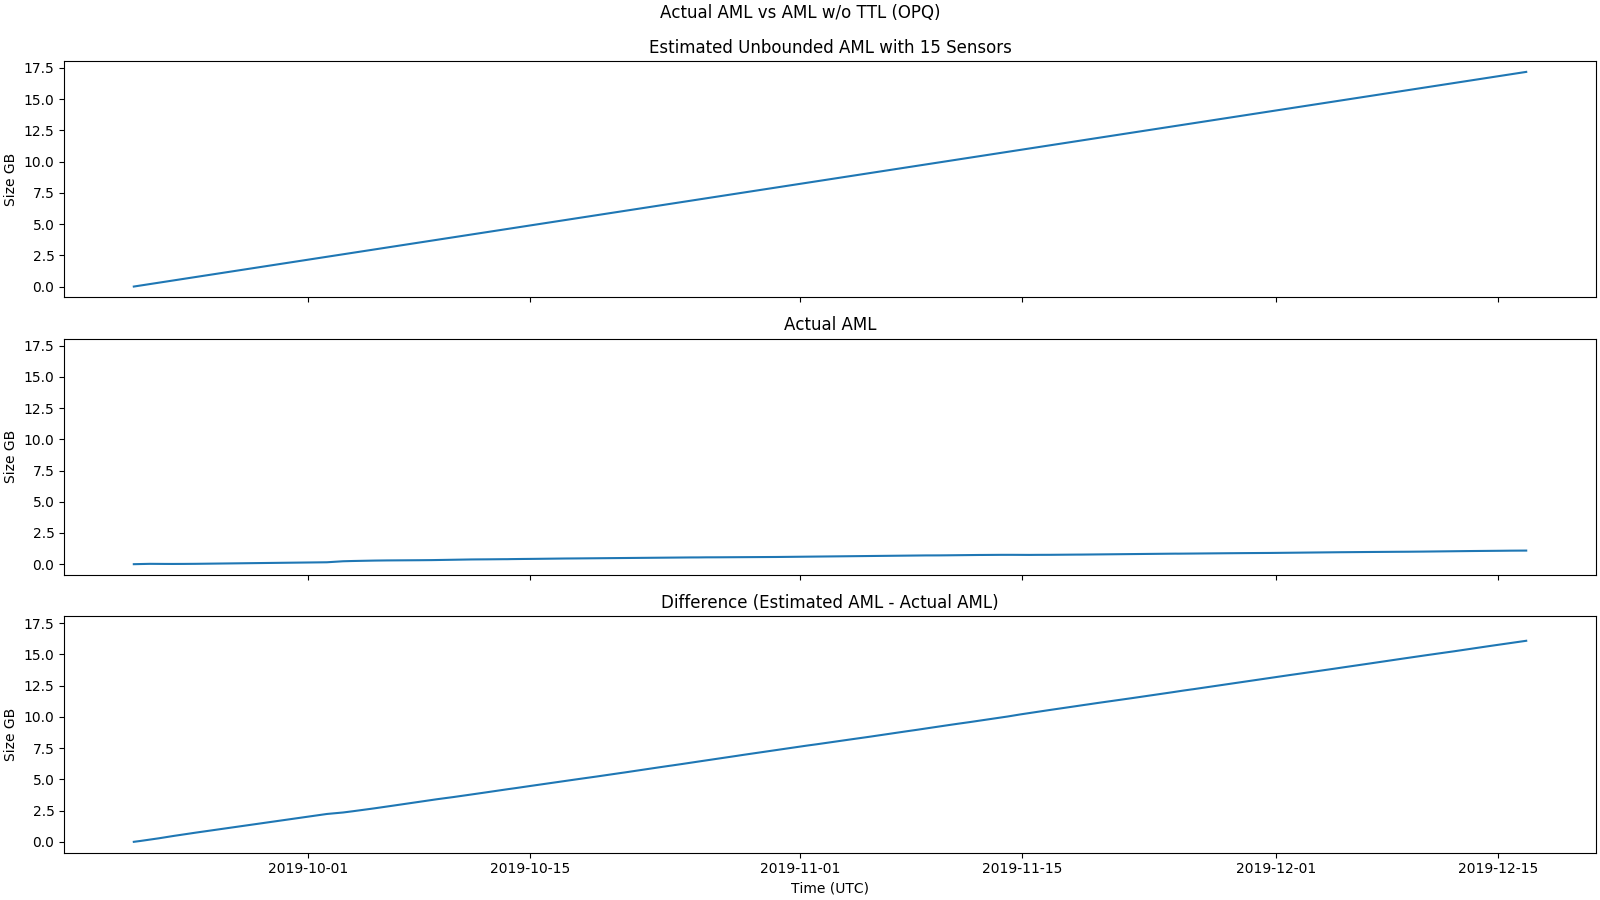
\includegraphics[width=\linewidth]{figures/actual_aml_vs_unbounded_opq.png}
    \caption{Actual AML vs Unbounded AML for OPQ}
    \label{fig:actual_aml_vs_unbounded_opq}
\end{figure}

This data was not affected by the implicit TTL parameter and portrays accurate unbounded versus bounded growth. We can see that over the same time period, AML with TTL saved us about 17.5 GB worth of data versus a store everything approach.

\paragraph{DL Versus Estimated Growth}
Figure~\ref{fig:actual_dl_vs_unbounded_opq} shows the actual DL vs unbounded DL. The Detection Level contains metadata and data bounded by a window which may or may not include signals of interest.

\begin{figure}[H]
    \centering
    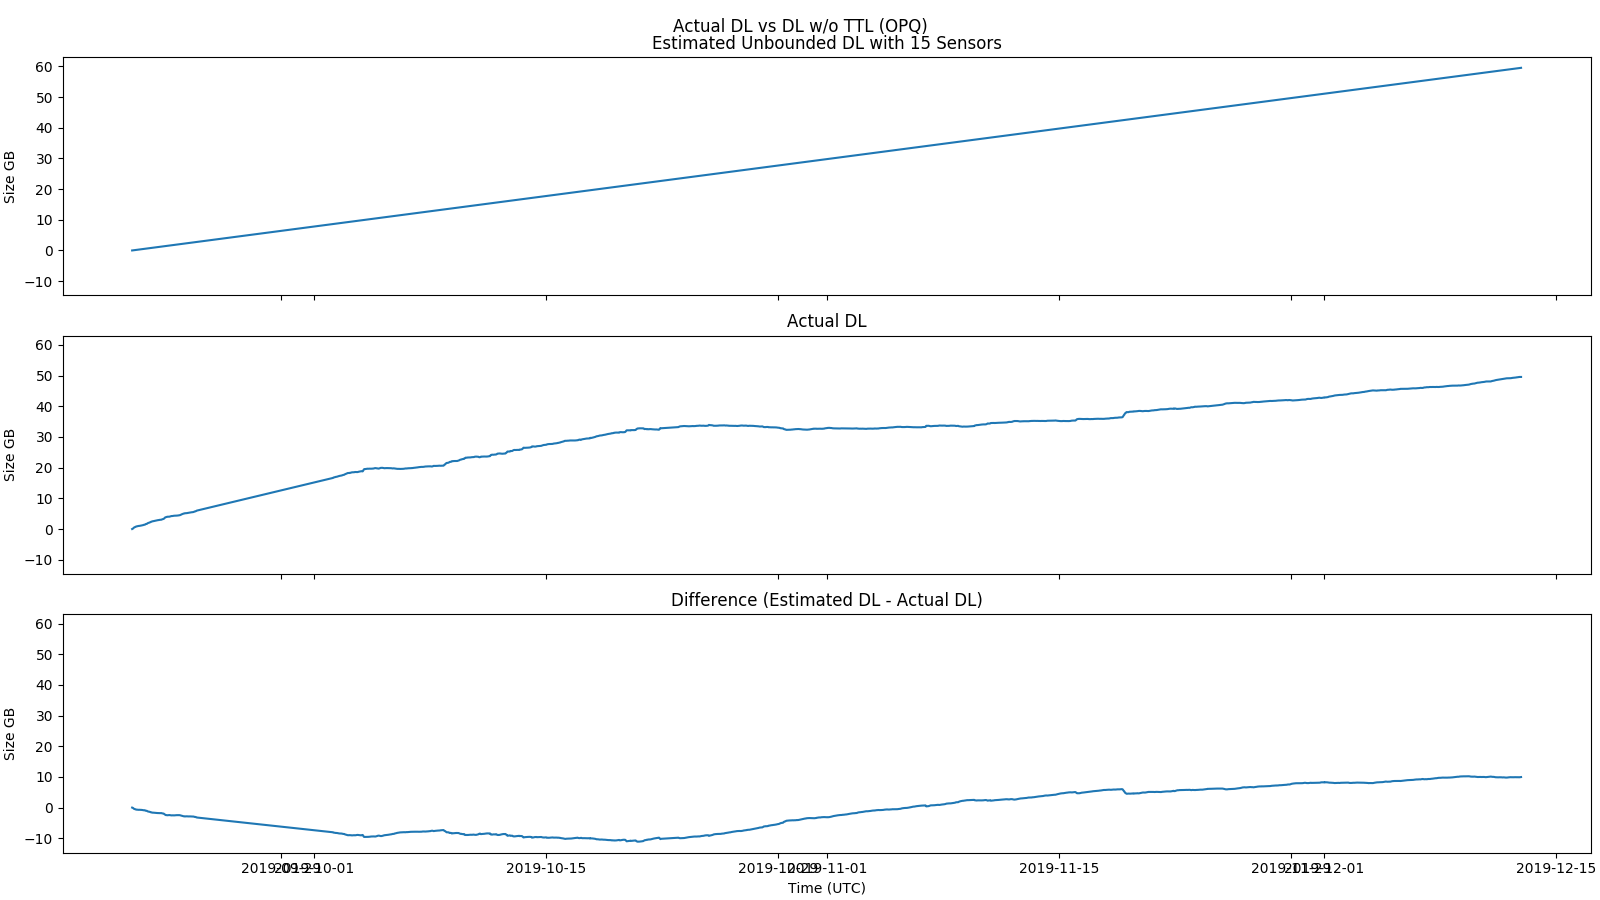
\includegraphics[width=\linewidth]{figures/actual_dl_vs_unbounded_opq.png}
    \caption{Actual DL vs Unbounded DL for OPQ}
    \label{fig:actual_dl_vs_unbounded_opq}
\end{figure}

This data was affected by the implicit TTL parameter and does not portray accurate unbounded versus bounded growth. Instead, the implicit TTL parameter models are actual growth pretty closely and the actual data is about 20 GB larger than the estimated data growth.

\paragraph{IL Versus Estimated Growth}
Figure~\ref{fig:actual_il_vs_unbounded_opq} shows the actual IL vs unbounded IL. The Incident Level contains metadata and data over window that contains classified signals of interest.

\begin{figure}[H]
    \centering
    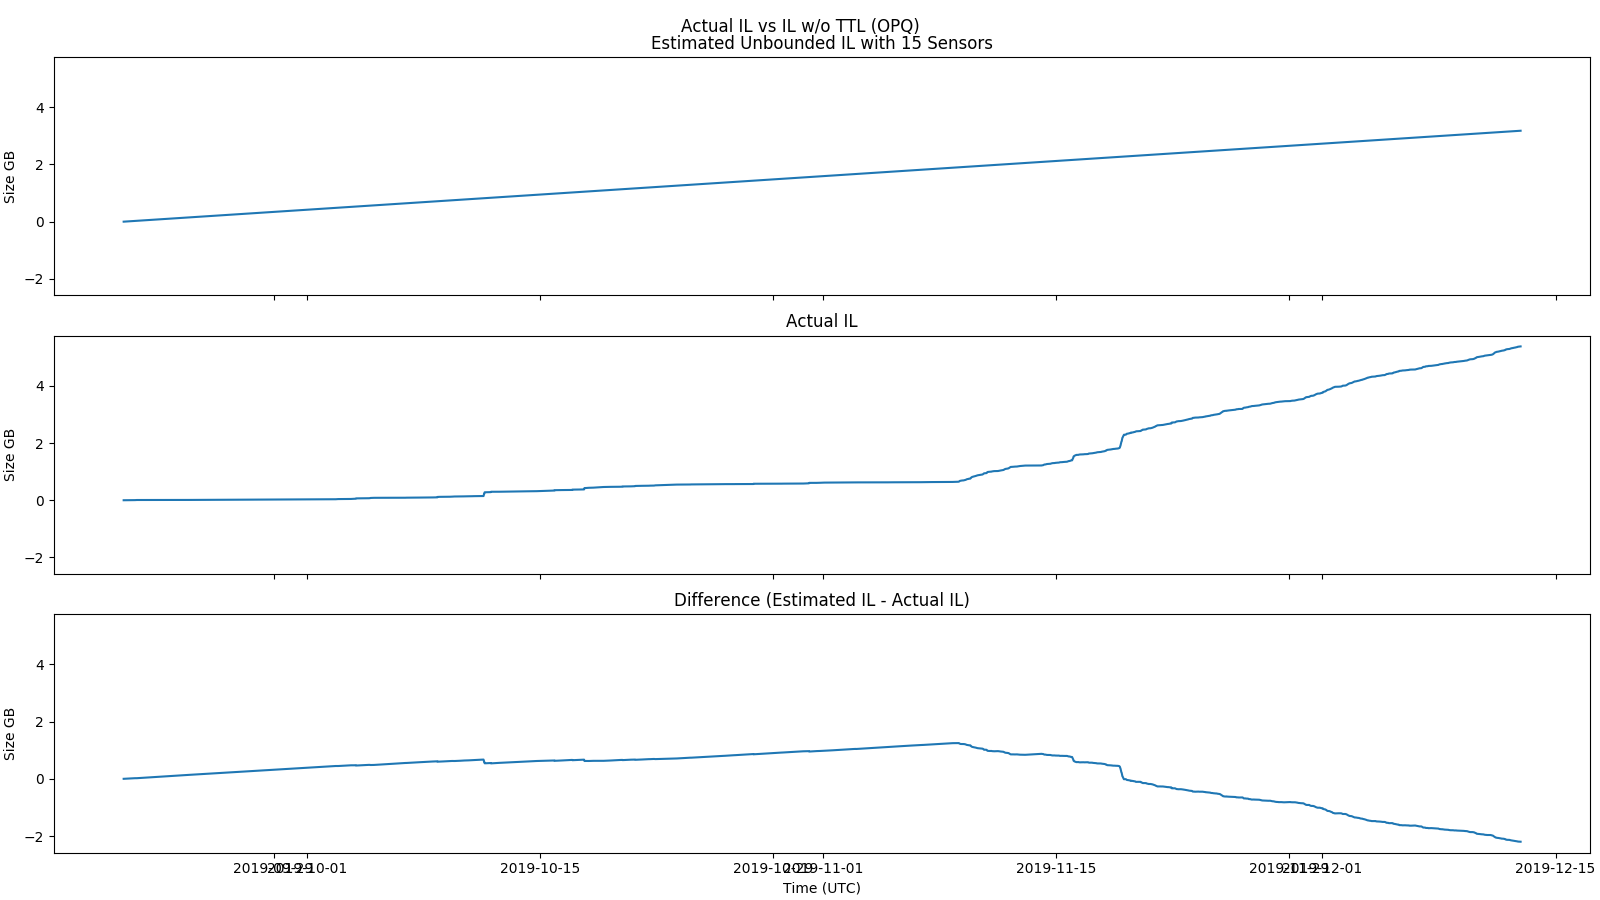
\includegraphics[width=\linewidth]{figures/actual_il_vs_unbounded_opq.png}
    \caption{Actual IL vs Unbounded IL for OPQ}
    \label{fig:actual_il_vs_unbounded_opq}
\end{figure}

This data was affected by the implicit TTL parameter and does not portray accurate unbounded versus bounded growth. Instead, we can see that the actual size of the IL tracks pretty closely to the estimated maximum bounds. At the end of the data collection period, OPQ collected about 4GB less worth of data than what was estimated.

\paragraph{PL Versus Estimated Growth}
Figure shows the actual PL vs unbounded PL.

% TODO
TODO

\paragraph{Laha Versus Estimated Growth}
Finally, I examine the total size of Laha and compare it to the estimated bounds of Laha without TTL. This takes into account all levels within the Laha hierarchy.

Figure~\ref{fig:actual_laha_vs_unbounded_opq} compares the actual bounds of the entire network to the estimated bounds.

\begin{figure}[H]
    \centering
    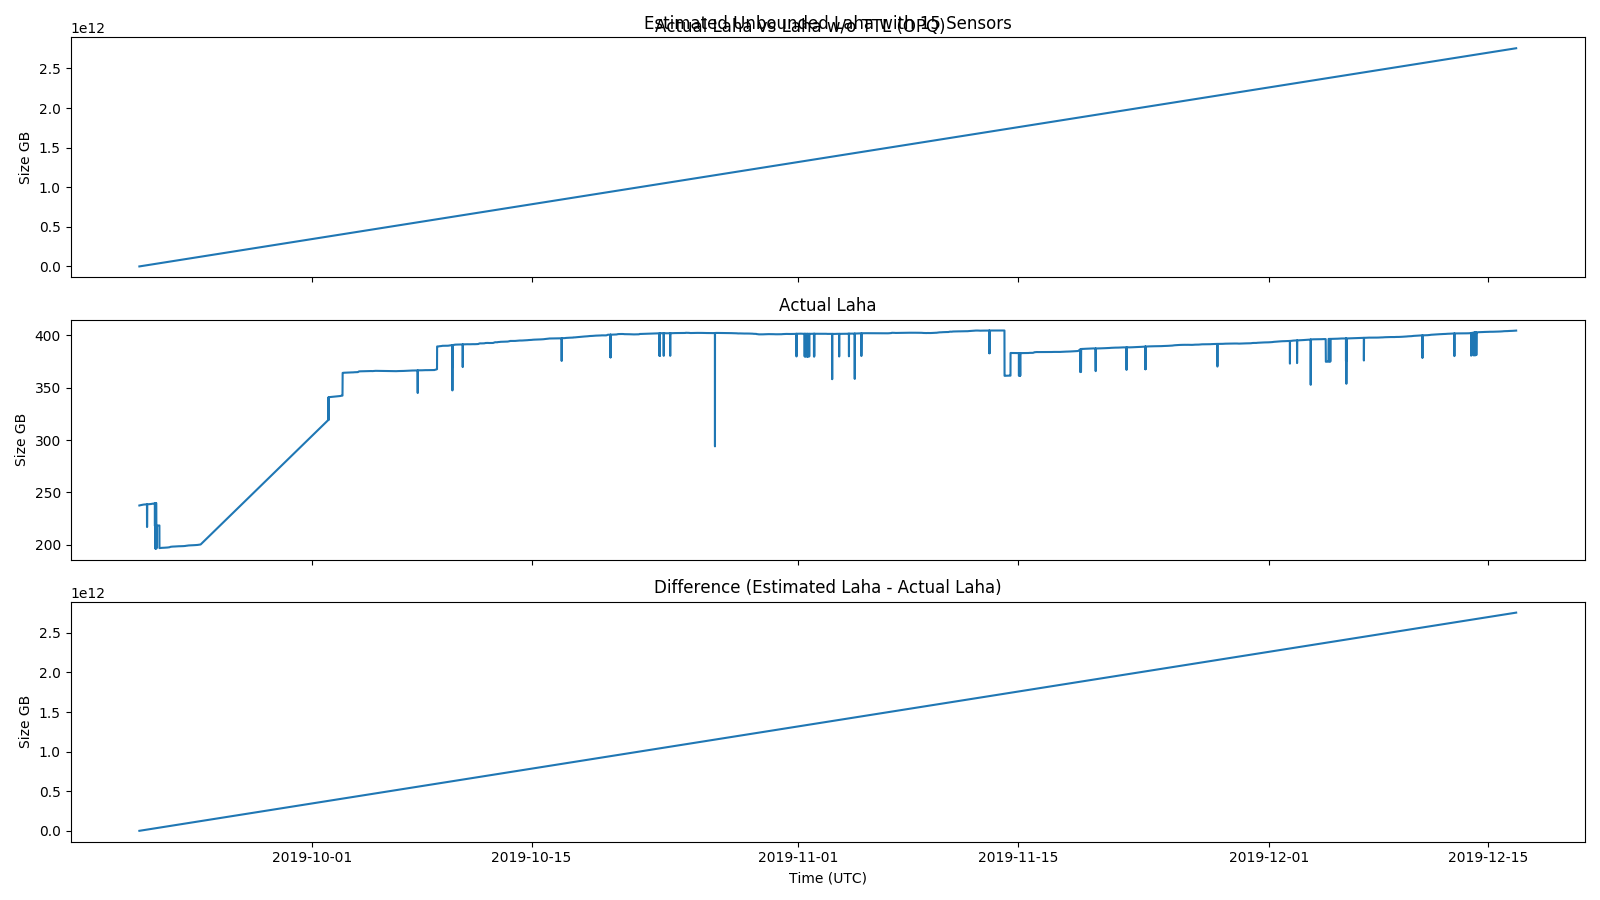
\includegraphics[width=\linewidth]{figures/actual_laha_vs_unbounded_opq.png}
    \caption{Actual Laha vs Unbounded Laha for OPQ}
    \label{fig:actual_laha_vs_unbounded_opq}
\end{figure}

This result is a little unsatisfying. The data growth of the IML is pretty much the only feature evident in this plot. To better understand the growth of the entire system, I removed the IML as shown in Figure~\ref{fig:actual_laha_vs_unbounded_no_iml_opq}.

\begin{figure}[H]
    \centering
    \includegraphics[width=\linewidth]{figures/actual_laha_vs_unbounded_opq_no_iml.png}
    \caption{Actual Laha vs Unbounded Laha for OPQ (No IML)}
    \label{fig:actual_laha_vs_unbounded_no_iml_opq}
\end{figure}

Over a time period of 2 and a half months, the OPQ network saved about 20GB of data as compared to a store everything approach (not including the IML which saved about 2.5 TB of data). Of course, I would expect this difference to be greater if I had actual metrics for the DL, IL and PL that did not have a built-in implicit TTL parameter. Even with the built-in parameter, the savings gained from the AML alone is significant.

\subsubsection{DSN System Requirements OPQ: Comparing Results to Simulated Data}

Next I will compare the results gathered from the OPQ deployment to the simulated bounds found in Section~\ref{sssec:evaluation_of_ttl}.

Similar to the previous comparisons, I will offset the actual data to ``force" the data to start from zero.

The simulated data had to be aligned with the collected metrics to perform this evaluation. The alignment works by binning all relevant timestamps to the nearest minute between the two data series.

\paragraph{IML Versus Simulated Growth}
The Instantaneous Measurements Level (IML) contains raw samples from sensors. Figure~\ref{fig:actual_iml_vs_sim_opq} shows the actual IML vs estimated IML.

\begin{figure}[H]
    \centering
    \includegraphics[width=\linewidth]{figures/actual_iml_vs_sim_opq.png}
    \caption{Actual IML vs Simulation IML for OPQ}
    \label{fig:actual_iml_vs_sim_opq}
\end{figure}

The simulation tracks the actual data pretty closely with a difference hovering around 0 MB. The simulation assumes that 15 sensors are always sending, whereas the actual data fluctuates with the number of active sensors.

\paragraph{AML Versus Simulated Growth}
The Aggregate Measurements Level (AML) contains rolled up summary statistics of selected features generated from IML data. Figure~\ref{fig:actual_aml_vs_sim_opq} shows the actual AML vs estimated AML.

\begin{figure}[H]
    \centering
    \includegraphics[width=\linewidth]{figures/actual_aml_vs_sim_opq.png}
    \caption{Actual AML vs Simulation AML for OPQ}
    \label{fig:actual_aml_vs_sim_opq}
\end{figure}

The simulated AML data trends closely with the actual data. There is a slight underestimation early on, but converges to close to 0 GB by the end of the data collection.

\paragraph{DL Versus Simulated Growth}
The Detection Level (DL) contains metadata and a window of raw data that may or may not include signals of interest. Figure~\ref{fig:actual_dl_vs_sim_opq} shows the actual DL vs estimated DL.

\begin{figure}[H]
    \centering
    \includegraphics[width=\linewidth]{figures/actual_dl_vs_sim_opq.png}
    \caption{Actual DL vs Simulation DL for OPQ}
    \label{fig:actual_dl_vs_sim_opq}
\end{figure}

Although the simulated data has a similar shape to the actual data for the DL, there is a large offset between the simulation and the actual data. There are several reasons for this offset. The parameters passed into the simulation have somewhat large variances. The leading issue though, is that the simulation assumes that each device produces the same amount of Detections. In practice, certain boxes produce many Detections while others produce relatively few Detections. These differences can likely be attributed to the offset. On the bright side, at least the actual data is less than the simulated data and not the other way around!

OPQ saves near 150 GB of data as compared to the simulation.

\paragraph{IL Versus Simulated Growth}
The Incidents Level (IL) contains metadata and a window of data that contains classified signals of interest. Figure~\ref{fig:actual_il_vs_sim_opq} shows the actual IL vs estimated IL.

\begin{figure}[H]
    \centering
    \includegraphics[width=\linewidth]{figures/actual_il_vs_sim_opq.png}
    \caption{Actual IL vs Simulation IL for OPQ}
    \label{fig:actual_il_vs_sim_opq}
\end{figure}

The simulated IL data is better than the simulated DL data, but still displays an offset, likely for the same reasons as the DL. OPQ saves 20 GB in the IL compared to the simulated IL.

\paragraph{PL Versus Simulated Growth}
Figure shows the actual PL vs estimated PL.

% TODO
TODO

\paragraph{Laha Versus Simulated Growth}
Figure~\ref{fig:actual_laha_vs_sim_opq} shows the actual Laha vs estimated Laha.

The large offsets in the simulated DL and IL data create the overall trends in this plot. The shapes of the trends are similar but the offset shows that OPQ saves near 150 GB of data over the same time period as the simulation.

\begin{figure}[H]
    \centering
    \includegraphics[width=\linewidth]{figures/actual_laha_vs_sim_opq.png}
    \caption{Actual Laha vs Simulation Laha for OPQ}
    \label{fig:actual_laha_vs_sim_opq}
\end{figure}

\paragraph{Discussion on Estimation Versus Simulation}

I compared actual data for each level in the Laha hierarchy to both estimated bounds and simulated bounds. Both approaches show promising results for certain levels. The estimated bounds are better suited for examining the DL, IL, and PL whereas the simulated bounds are better for examining the IML and AML. The estimated bounds include an implicit TTL parameter where the simulated bounds actually performs TTL in the simulation.

One thing that the simulation provides is the ability to tune many of the underlying simulation parameters. The estimated data provides parameters scraped from the database and if a fairly simply estimation. The simulation allows individual parameters to be tuned providing the means to alter any part of a simulated Laha DSN. This is something that is not easily accomplished only using estimation methods.

Future work should look at expanding the collection of parameters saved when items are garbage collected. This would allow better estimated bounds without TTL and provide better parameters to the simulation.

Both approaches showed significant data savings when utilizing the data management techniques within Laha.

\subsubsection{DSN System Requirements OPQ: CPU, Memory, and Disk Utilization}

We collected CPU, memory, and disk utilization during the deployment of the OPQ network. It is useful to first discuss the details of the system that the OPQ network is running on.

Makai, Mauka, View, MongoDB, and Health are all running on the same virtual server hosted by the University's Information Technology Services. The server is running Red Hat Enterprise Linux Server release 7.7 (Maipo). Due to a configuration error, the server only ran with a single virtual CPU up until October 28, 2019. After that time period, a second virtual CPU was added. Each virtual CPU is an Intel Xeon E5-2687W v3 running at 3.10 GHz. The system has 8 GB of main memory and 8 GB of swap space. The system has 1 TB of hard disk storage.

These system statistics are for the entire virtual server and include loads of all virtualized OPQ services. Mauka is certainly doing the most work of any of the virtualized services, but it should be noted that these statistics also include overhead incurred from other OPQ and OS services.

It should be noted that I attempted to collect the same statistics from the Lokahi network, but due to system requirements and a complicated distributed architecture, we were not able to collect metrics for the entire system. For example, many of Lokahi's services use specialized Amazon Web Services (AWS) services which do not expose similar metrics that are exposed by OPQ. For that reason, we will only examine the OPQ network in detail.

Figure~\ref{fig:actual_system_opq} shows the OPQ system resource utilization over a period of two and a half months.

\begin{figure}[H]
    \centering
    \includegraphics[width=\linewidth]{figures/actual_system_opq.png}
    \caption{System Utilization for OPQ}
    \label{fig:actual_system_opq}
\end{figure}

You'll note gaps in the data in early and mid October. These were caused by a mix-up in deployed branches where one of the branches did not have collection of system statistics enabled.

The top panel shows the minimum, mean, and maximum CPU load. Each triplet of min, mean, and max values are aggregated over 30 sample points. So even though the CPU hits 100\% utilization quite often, the mean of the CPU utilization is much lower, rarely rising over 40\%. A slight decrease (~5\%) in CPU load can be observed when the second virtual CPU was added to the system.

I expect that we could double the amount of deployed sensors to 30 and still see mean CPU utilization less than 80\%. Beyond that would require either more powerful hardware or distributing OPQ services over multiple servers.

The second panel shows memory utilization. OPQ utilizes on average close to 75\% of the available memory. I dug a little bit deeper into how the memory was being utilized and found a perhaps unsurprising result. Table~\ref{table:mem_utilization} shows the breakdown of largest memory utilization on our system.

\begin{table}[H]
    \centering
    \caption{OPQ Large Memory Utilization}
    \begin{tabularx}{\textwidth}{Xl}
        \toprule
        \textbf{Process} & \textbf{\% Memory} \\
        \midrule
        MongoDB & 51 \\
        OPQ Mauka & 8 \\
        OPQ View & .8 \\
        OPQ Makai & .3 \\
        Docker & .3 \\
        OPQ Box Updater & .1 \\
        JournalD & .1 \\
        \bottomrule
    \end{tabularx}
    \label{table:mem_utilization}
\end{table}

MongoDB uses over half of our available memory! This should be somewhat unsurprising because MongoDB aggressively caches data in-memory for efficient queries. No matter how much memory is on our system, MongoDB will use a large chunk of it. All of the OPQ Mauka processes combined only add up to about 8\% memory utilization with 15 sensors. I estimate that on current hardware, Mauka could handle up to about 100 sensors and still remain within 80\% memory utilization (of course this would have an adverse affect on MongoDB caching).

The third panel shows disk usage over time. As of about two and a half months into data collection, the server is storing about 130 GB worth of data. One interesting feature of this plot are the periodic spikes. The periodic spikes are caused by daily database backups. Every day, a backup of the database is performed, compressed, and written to disk. It is then uploaded to cloud storage and on successful upload, deleted locally. There is a large gap of these spike near the end of October and beginning of November. This gap is the result of a Docker bug that inhibited our system from performing daily backups. I changed the backup routine to use a local MongoDB client rather than one provided by Docker and the daily backups resumed.

The bottom panel shows the number of active OPQ Boxes sending over time. There does not appear to be a large correlation between the number of boxes sending and system resource utilization. This is likely due to the fact that the standard deviation between the number of active OPQ Boxes is quite small ($\sigma=1.63$).

\subsection{DSN System Requirements: Lokahi}\label{subsec:dsn-system-requirements:-lokahi}

The requirements of the Lokahi network stipulate that all data be saved. This is broadly due to the fact that many of our collaborators request data long after it would have been garbage collected by TTL. Because of this requirement, TTL was not implemented for the Lokahi network. I believe this is a feature, not a bug. This gave me the opportunity to compare a network that does utilize TTL (OPQ) to a network that does not utilize TTL (Lokahi). Evaluations for these results are provided in Sections~\ref{sssec:eval_of_dsn_system_requirements} and~\ref{sssec:evaluation_of_ttl}.

I've shown in the previous section the data savings OPQ experienced against estimated data growth and simulated data growth. In this section, I will show the amount of data actually stored in Lokahi versus how much data could have been saved using TTL. This will compare the actual data collected from the Lokahi network to the estimated and simulated data found in the Evaluation chapter.

Data was scraped from the Lokahi servers over the same time period as the OPQ data, October 1 to December 15, 2019. The first sample of all data sets are subtracted from subsequent data in order to ``zero out" the data at the origin and show data growth from zero rather than data growth from an unknown previous point.

\subsubsection{DSN System Requirements Lokahi: IML}

The Instantaneous Measurements Level (IML) contains raw samples collected by sensors. Because Lokahi does not utilize a TTL, the IML data is stored indefinitely. Here, I only consider IML data collected by microphone sensors which is the focus of the Lokahi deployment.

Figure~\ref{fig:active_lokahi_sensors} shows the number of active Lokahi sensors at different sampling rates over the period of the deployment.

\begin{figure}[H]
    \centering
    \includegraphics[width=\linewidth]{figures/lokahi_num_sensors.png}
    \caption{Active Lokahi Sensors}
    \label{fig:active_lokahi_sensors}
\end{figure}

The above Figure shows the number of active Lokahi sensors at different sampling rates. Unlike OPQ, the Lokahi network provides sensors that can be configured to sample at 80, 800, or 8000 Hz depending on the target signal of interest. Differences in sampling rates affect both the IML and the AML. IML data is affected because more samples require more storage. The AML is affected because Trend rates are dependent on the sampling rate. At any one time, the Lokahi network observed a mean of close to 100 active sensors. Sensors recording at 800 Hz are most prevalent, followed by sensors at 80 Hz, and finally sensors at 8000 Hz.

Figure~\ref{fig:lokahi_actual_iml} shows the actual data growth of the IML over the course of the Lokahi deployment.

\begin{figure}[H]
    \centering
    \includegraphics[width=\linewidth]{figures/lokahi_actual_iml.png}
    \caption{IML Growth: Lokahi}
    \label{fig:lokahi_actual_iml}
\end{figure}

A linear regression has been fitted to the total IML growth size and is provided by Equation~\ref{eq:lokahi_iml_lr}.

\begin{equation}
    y = 0.0002934630429487022 * x + -460888.760172118
    \label{eq:lokahi_iml_lr}
\end{equation}

Most of the IML data is made up of 800 Hz sampled data. This is unsurprising since most active sensors are sampling at 800 Hz. Over a period of two and a half months, the total IML size reaches near 2 TB.

Next, I will examine how the actual data compares to the estimated data and the simulated data found in the Evaluation chapter.

Figure~\ref{fig:lokahi_actual_iml_vs_est} compares the estimated IML data to the actual IML data.

\begin{figure}[H]
    \centering
    \includegraphics[width=\linewidth]{figures/lokahi_actual_iml_vs_est.png}
    \caption{IML Growth: Estimated vs Actual}
    \label{fig:lokahi_actual_iml_vs_est}
\end{figure}

As can be observed, the estimated IML data ends up being close to 1 TB larger than that of the actual IML data. This is attributed to the fact that the estimated data only works with the mean number of active sensors whereas the actual data uses the actual number of active sensors.

Figure~\ref{fig:lokahi_actual_iml_vs_sim} compares the simulated IML data to the actual IML data.

\begin{figure}[H]
    \centering
    \includegraphics[width=\linewidth]{figures/lokahi_actual_iml_vs_sim.png}
    \caption{IML Growth: Simulated vs Actual}
    \label{fig:lokahi_actual_iml_vs_sim}
\end{figure}

Here, the simulated data shows data savings of near 2 TB. This makes sense because the simulated data utilizes TTL whereas the actual Lokahi network does not. This provides evidence that TTL within the IML provides for significant data savings.

\subsubsection{DSN System Requirements Lokahi: AML}

The Aggregate Measurements Level (AML) stores summary statistics from feature extracted streams and metadata relating to the data streams. In Lokahi, the AML only contains Trends whereas OPQ contains both Measurements and Trends. Trend rates vary depending on IML sampling rate.

Figure~\ref{fig:lokahi_actual_aml} shows the actual AML growth of the Lokahi network over its deployment.

\begin{figure}[H]
    \centering
    \includegraphics[width=\linewidth]{figures/lokahi_actual_aml.png}
    \caption{AML Growth: Lokahi}
    \label{fig:lokahi_actual_aml}
\end{figure}

Equation~\ref{eq:lokahi_aml_lr} provides the linear regression found for the total AML data growth.

\begin{equation}
    y = 5.309751501193485e-06 * x + -8339.047270943533
    \label{eq:lokahi_aml_lr}
\end{equation}

Over the course of the Lokahi deployment, the total size of the AML grew to just over 35 GB.

Next, I will examine how the actual data compares to the estimated data and the simulated data found in the Evaluation chapter.

Figure~\ref{fig:lokahi_actual_aml_vs_est} shows the estimated AML versus the actual AML.

\begin{figure}[H]
    \centering
    \includegraphics[width=\linewidth]{figures/lokahi_actual_aml_vs_est.png}
    \caption{AML Growth: Estimated vs Actual}
    \label{fig:lokahi_actual_aml_vs_est}
\end{figure}

Actual AML data ends up being about 15 GB smaller that the estimated data. Again, this is likely caused by the fact that the estimated data uses the mean number of active sensors while the actual data uses the actual number of active sensors for any period of time.

Figure~\ref{fig:lokahi_actual_aml_vs_sim} shows the simulated AML compared to the actual AML.

\begin{figure}[H]
    \centering
    \includegraphics[width=\linewidth]{figures/lokahi_actual_aml_vs_sim.png}
    \caption{AML Growth: Simulated vs Actual}
    \label{fig:lokahi_actual_aml_vs_sim}
\end{figure}

Simulated data provides upwards of 20 GB in data savings utilizing TTL compared to the actual AML data which does not utilize TTL. This provides evidence that a TTL approach could provide significant data savings for the AML.

\subsubsection{DSN System Requirements Lokahi: DL}

The Detections Level (DL) is responsible for bounding data with a window that may or may not contain signals of interest. Figure~\ref{fig:lokahi_actual_dl} shows the actual growth of the DL within Lokahi over the deployment duration.

\begin{figure}[H]
    \centering
    \includegraphics[width=\linewidth]{figures/lokahi_actual_dl.png}
    \caption{Lokahi DL Growth}
    \label{fig:lokahi_actual_dl}
\end{figure}

Equation~\ref{eq:lokahi_dl_lr} provides the linear regression found for the total DL data growth.

\begin{equation}
    y = 4.241184190694421e-07 * x + -0.29152838226742694
    \label{eq:lokahi_dl_lr}
\end{equation}

Over the deployment duration, the DL has grown over 2.5 GB with over 200 Events.

Next I will compare the actual DL data growth to the estimated and simulated data growth from the Evaluation chapter. Figure~\ref{fig:lokahi_actual_dl_vs_est} compares the actual Lokahi DL to the estimated DL.

\begin{figure}[H]
    \centering
    \includegraphics[width=\linewidth]{figures/lokahi_actual_dl_vs_est.png}
    \caption{Lokahi DL Growth vs Estimated Growth}
    \label{fig:lokahi_actual_dl_vs_est}
\end{figure}

The actual DL growth matches the estimated DL growth almost perfectly. The difference between the two trends towards 0 GB.

Figure~\ref{fig:lokahi_actual_dl_vs_sim} compares the simulated DL to the actual DL.

\begin{figure}[H]
    \centering
    \includegraphics[width=\linewidth]{figures/lokahi_actual_dl_vs_sim.png}
    \caption{Lokahi DL Growth vs Simulated Growth}
    \label{fig:lokahi_actual_dl_vs_sim}
\end{figure}

The simulated DL is about 1.5 GB smaller than the actual DL. This is due to the simulated DL utilizing TTL while the actual DL for Lokahi does not. This provides evidence that TTL based approaches can provide data savings within the DL.

\subsubsection{DSN System Requirements Lokahi: IL}

The Incidents Level (IL) is responsible for bounding data with a window that contains classified signals of interest. Figure~\ref{fig:lokahi_actual_il} shows the actual growth of the IL within Lokahi over the deployment duration.

\begin{figure}[H]
    \centering
    \includegraphics[width=\linewidth]{figures/lokahi_actual_il.png}
    \caption{Lokahi IL Growth}
    \label{fig:lokahi_actual_il}
\end{figure}

Equation~\ref{eq:lokahi_il_lr} provides the linear regression found for the total IL data growth.

\begin{equation}
    y = 1.982441768799792e-08 * x + -0.02980347263345723
    \label{eq:lokahi_il_lr}
\end{equation}

Over the deployment duration, the IL has grown to about 0.125 GB consisting of 6 Incidents. Incidents are much more rare in Lokahi as compared to OPQ.

Next I will compare the actual IL data growth to the estimated and simulated data growth from the Evaluation chapter. Figure~\ref{fig:lokahi_actual_il_vs_est} compares the actual Lokahi IL to the estimated IL.

\begin{figure}[H]
    \centering
    \includegraphics[width=\linewidth]{figures/lokahi_actual_il_vs_est.png}
    \caption{Lokahi IL Growth vs Estimated Growth}
    \label{fig:lokahi_actual_il_vs_est}
\end{figure}

The actual IL trends closely with the estimated IL.

Figure~\ref{fig:lokahi_actual_il_vs_sim} compares the simulated IL to the actual IL.

\begin{figure}[H]
    \centering
    \includegraphics[width=\linewidth]{figures/lokahi_actual_il_vs_sim.png}
    \caption{Lokahi IL Growth vs Simulated Growth}
    \label{fig:lokahi_actual_il_vs_sim}
\end{figure}

The simulated IL is just slightly smaller than the actual IL. Over this time period, the simulated IL does not have a good opportunity to show off the data savings provided by TTL. I suspect that if the deployment were long enough, we would see similar simulated data savings to what was displayed for the IML, AML, and DL. Although the simulated TTL is not in use here, Laha is designed to work for extremely long durations. In those scenarios, the larger TTL of Incidents will come into play.

\subsubsection{DSN System Requirements Lokahi: PL}

% TODO
TODO

\subsubsection{DSN System Requirements Lokahi: Laha}

Figure~\ref{fig:lokahi_actual_laha} shows the total size of all levels collected from actual data from the Lokahi network.

\begin{figure}[H]
    \centering
    \includegraphics[width=\linewidth]{figures/lokahi_actual_laha.png}
    \caption{Lokahi Laha Growth}
    \label{fig:lokahi_actual_laha}
\end{figure}

The total size of the Lokahi deployment reaches close to 2 TB over two and a half months. This is mostly due to the large IML that this network produces. Next I will compare the total size of Laha to the estimated and simulated results from the Evaluation chapter.

Figure~\ref{fig:lokahi_actual_laha_vs_est} shows actual Laha growth compared to estimated Laha growth.

\begin{figure}[H]
    \centering
    \includegraphics[width=\linewidth]{figures/lokahi_actual_laha_vs_est.png}
    \caption{Lokahi Laha Growth vs Estimated Laha Growth}
    \label{fig:lokahi_actual_laha_vs_est}
\end{figure}

The actual data growth of Laha is close to 1 TB smaller than that of the estimated data growth. This should come as no surprise since these match estimated results for all of the sub-levels that make up the Laha hierarchy.

Figure~\ref{fig:lokahi_actual_laha_vs_sim} shows actual Laha growth versus simulated Laha growth.

\begin{figure}[H]
    \centering
    \includegraphics[width=\linewidth]{figures/lokahi_actual_laha_vs_sim.png}
    \caption{Lokahi Laha Growth vs Simulated Laha Growth}
    \label{fig:lokahi_actual_laha_vs_sim}
\end{figure}

The estimated data growth of Laha for Lokahi ends at close to 2 TB smaller that the actual data growth. As discussed for the previous levels, this is due to the fact that Lokahi doesn't implement TTL whereas the simulated does implement TTL. This provides evidence that a TTL approach would be useful in networks similar to Lokahi to achieve substantial data savings.

In this section, I have compared the actual amount of data collected to estimated data and simulated data outlined in the Evaluation chapter. The estimated data tends to be slightly larger than the actual data for all instances. This difference was caused by errors in the estimations due to utilizing the mean number of active sensors rather than the actual number of active sensors. The simulated results showed that a TTL approach would be useful in providing data savings.

\section{Results of Tertiary Goals}\label{sec:results-of-tertiary-goals}

In the introduction Section~\ref{subsec:tertiary-goals-and-claims}, I provided tertiary goals for the Laha framework. The evaluation of these tertiary goals were provided in Section~\ref{sec:evaluation-of-tertiary-goals}. In general, two out of the three tertiary goals were implemented to some degree. Not all of the results mentioned in the Evaluation chapter for the tertiary goals were fulfilled. This section examines to what extent the tertiary goals were fulfilled and discusses how these results might be improved.

\subsection{Results of Adaptive Optimizations for Triggering}\label{subsec:results-of-adaptive-optimizations-for-triggering}

In the previous discussion on Future Phenomena, I showed how Future Phenomena have the ability to modify the Measurement and Trend rates for OPQ Boxes. These rates are increased over the duration that a Future Phenomena signal is predicted. The measurement rate is increased from one Measurement per 60 cycles to one Measurement per 10 cycles. Once the Future Phenomena duration ends, the rates are adjusted back to default values.

This increase in fidelity provides triggering algorithms with more data to work with and provides a smaller window ($\frac{1}{6}$ of a second compared to 1 second) in which deviations can be identified. This increases the network's chance of observing Events and Incidents that may have originally been missed.

The increased fidelity during Future Phenomena adds a small overhead cost in terms of bandwidth and storage. As shown in the Evaluation of Tiered Management of Big Data chapter, the mean size of a Measurement is 145 bytes. The added overhead can be found by Equation~\ref{eq:added_overhead} where $P_i$ is a given Future Phenomena and $D$ is a function that returns the duration of the Phenomena in seconds.

\begin{equation}
    added\_overhead\_bytes = \sum_{i=1}^{P_{N}} D(P_i) * 145 * 6
    \label{eq:added_overhead}
\end{equation}

Over a period of one week, 772 Future Phenomena were created for four OPQ Boxes. These contributed to an increase of 130.51 MB of data transferred from OPQ Boxes under Future Phenomena. Considering that four OPQ Boxes transfer 365.50 MB in Measurements and Trends without Future Phenomena, this is about a 35\% increase in data transfer for OPQ Boxes utilizing Future Phenomena for adaptive triggering optimizations.

These optimizations were designed to increase fidelity and reduce window size, providing triggering algorithms the chance to better identify Events. Future directions should include looking to information theory for ideas on how to decrease fidelity while still maintaining a high signal-to-noise ratio. Another future direction should experiment with modifying the sampling rates of the sensors themselves to determine if possible to decreases bandwidth and storage requirements while increasing signal-to-noise.

\subsection{Results of Adaptive Optimizations for Detection and Classification}\label{subsec:results-of-adaptive-optimizations-for-detection-and-classification}

In the previous discussion on Future Phenomena, I showed that Future Phenomena are capable of optimizing the classification of Events by dynamically modifying the feature thresholds used for detecting Events. This is in contrast to what I claimed I would do in the Evaluation section which stated that I would change the window sizes to dynamically increase or decrease signal-to-noise.

I decided to switch directions with optimizations for Events because the time windows for Events and Incidents are already well characterized and I don't believe modifying these windows would provide any additional benefits. For instance, Event windows are characterized by the times that thresholds crossed from nominal into non-nominal and back. We could increase the size of the Event window to provide a buffer of data on either end, but Event windows are already large enough to provide valid Incidents. Incident windows are strictly defined by the start and stop of the classified signal. If Incident windows were smaller, we would miss data that is important to characterizing the Incident. The Incident window does not need to be increased, because the Incident data is a subset of the Event data. The Event waveform will live for as long as the Incident, making it possible to look up data around the Incident from the Event that generated it.

I decided to dynamically alter detection thresholds in an attempt to provide Event detection with the ability to detect sub-threshold Events predicted by Future Phenomena that would have otherwise not been detected.

As discussed in the Results for Future Phenomena, out of 210 Future Phenomena, 37 Events were sub-threshold and would not have been identified without these adaptive optimizations.

Future directions should look at providing a signal-to-noise parameter that is used to dynamically adjust detection thresholds based on the required signal compared to the noise of a particular data stream.

\subsection{Results of Model of Underlying Sensor Field Topology}\label{subsec:results-of-model-of-underlying-sensor-field-topology}

I had difficulties finding a model that accurately predicts the underlying sensor field topology and as such do not have any results for this tertiary goal. I attempted to use Voltage sags and swells because they tend to show the largest differences in readings between Boxes at any one time. This is compared to THD and Frequency which tend to track more similarly between Boxes. I expected the signal caused by Voltage fluctuations to attenuate as a function of the distance from the source signal. This in conjunction with a map of the UH micro-grid provided the basis for me to explore this hypothesis.

I attempted to find the amount of ``hops" from each OPQ Box to every other OPQ Box on the UHM micro-grid. I did this by counting the number of buildings each main electrical line went through in order to go from an OPQ Box to every other OPQ Box. The UHM micro-grid is serviced by two sub-stations, one on upper campus and one on lower campus. This complicated counting the hops because different electrical routes are taken dependent on the substation that was servicing the micro-grid at any one time. I do not have any information on when each substation was active.

I compared the number of hops to the amount of attenuation observed in Voltage signals and was not able to identify any clear correlation. For certain pairs of sensors, the data made sense, but the correlation broke down for the vast majority of Voltage signals analyzed using this method leading me to believe that the small set of data points that did make sense are likely just coincidence.

There are also a lot of electrical switches, filters, and transformers that exist between each building and sometimes within buildings that further complicate counting hops. Also, just because a sensor observes a large Voltage signal that attenuates as it reaches other sensors does not mean that the source signal originated at the sensor with the largest signal. It could have originated in a near by building that does not have a OPQ Box inside of it.

I think one of the largest issues with this tertiary goal is my lack of knowledge relating to electrical engineering. I simply don't understand the movement of electricity within a grid well enough to be able to model the topology of the grid correctly only based off of Voltage signals and a map of the grid.

Although the OPQ Box deployment attempts to cover large parts of the campus, a larger deployment would make it much easier to follow signals as they propagate through the micro-grid. I suspect that a Box per building would almost make this a trivial problem, even with my lack of knowledge in the electrical engineering domain.

Multiple commercial software packages provide electrical grid simulation. It would be interesting to attempt to convert provided blueprints of the UHM micro-grid into a power grid simulation. With the ability to control signal sources, amplitudes, and locations of simulated sensors, I suspect this would provide an enlightening view of how power signals propagate through a grid. This could provide a fascinating future study on how and where renewable energy sources affect PQ based on the topology of the grid.

\subsection{Summary of Tertiary Goals}\label{subsec:summary-of-tertiary-goals}

I detailed 3 tertiary goals in the Evaluation chapter including adaptive optimizations of triggering, adaptive optimizations of detections and classification, and attempting to model the topology of a sensor field. I showed that adaptive triggering optimizations occur in the form of modifying data rates from OPQ Boxes. I showed that adaptive detection optimizations occur in the form of modifying detection thresholds. I was not able to provide a valid result for modeling the topology of the sensing field, but instead provides discussions on those results could be improved.

\section{Summary of Results}\label{sec:summary-of-results}

I designed, built, and deployed two Laha compatible DSNs. The Lokahi network collects signals in the infrasound range and is able to identify a large variety of source modalities such as rocket launches, earthquakes, atmospheric entries, storms, and explosions. The OPQ network was designed to detect anomalous signals in PQ data such as Frequency sags and swells, Voltage sags and swells, transients, and excessive THD.

I evaluated these DSNs as described in the Evaluation chapter.

First, I showed results comparing ground truth data to the OPQ network. I showed comparisons for collected metrics such a Frequency, Voltage, and THD, and I also provided results that compare how well Events and Incidents match what was observed by ground truth sensors. I found that most of the OPQ network accurately track the ground truth data with the largest deviations taking place within Frequency Incidents.

Next, I provided evidence to show how well Lokahi tracks ground truth data. I used results from Asmar's dissertation to show that infrasound signals are able to be detected with mobile sensors within accordance of the International Monitoring System.

I then provided results showing that the generality of Laha framework allows it to be used in multiple domains all the while fulfilling the requirements of those domains. Within the OPQ network, I showed examples of classified Incidents for common PQ issues and the ability to detect local, semi-global, and global signals-of-interest. Within the Lokahi network I provided Incidents that showcase the wide variety of source signal modalities that the network is able to accurately detect. Finally, I provided other tangible claims showing the usefulness and generality of the Lokahi network.

I then provided an in-depth discussion on the types of DSNs that the Laha framework would be suitable followed by a discussion on the Laha level hierarchy.

Next, I provided evidence that the system is able to convert primitive data into actionable insights by discussing the transformations of data at each level in the Laha hierarchy and examining the results of Phenomena which directly provide actionable insights. I examined each Phenomena is detail and discussed what value it adds and how it is able to optimize the underlying system.

Then, I provided results for tiered management of big data which focused on determining data storage requirements and system requirements in systems with TTL and without TTL. I compared results scraped from the data to estimations and simulations that were designed in the Evaluation chapter. I showed that Laha is able to reduce storage and computational requirements by removing noise from the system using garbage collection.

Finally, I provided results of the tertiary goals stated in the Evaluation chapter. I showed that adaptive optimizations of both triggering and detections take place and help to further improve the system's accuracy.

These items provide evidence that the Laha framework is a generally useful framework for distributed sensor networks in select domains, providing data storage management, actionable insights, and self-optimizing capabilities.

\section{Future Directions}\label{sec:future-directions}

The longer I've had to work with these networks, the more I realized that they could be expanded in a multitude of ways.

I think the lowest hanging fruit for Laha is to implement a machine learning layer. I believe machine learning could be used for triggering, detection, and classification of signals of interest. This is an active area of research within the Lokahi network as we are currently planning to augment our architecture with machine learning over the year of 2020. The goals for machine learning within Lokahi are to implement robust detection algorithms using a training set of labeled data collected at our lab and at various national laboratories.

I also believe machine learning could be useful at the Phenomena level, providing models for predicting Events and Incidents and identifying groupings of data. It would be great to augment Annotation Phenomena with the ability to automatically create new Annotations from past data.

In terms of creating Events and Incidents, I believe it would be useful to experiment with changing window sizes used to compute low level metrics such as Frequency, THD, and Voltage. As shown in the ground truth analysis, the current implementation uses cycle sized windows for computing THD and Frequency with the cost of added noise. These window sizes should me modified to find an optimum length that minimizes noise but still accurately reflects the data.

Although I created a simulation to simulate Laha itself, I believe it would be useful to simulate the power grid as well. Multiple commercial options exist that provide grid simulations. It would be useful to create a copy of the UHM micro-grid in simulation to help fill in some of the missing puzzle pieces about sensor topology and how signals travel through the UHM micro-grid. This would also afford us the opportunity to simulate PQ signals at will instead of waiting for them to arrive.

I would like to experiment with adding and/or combining levels within the Laha hierarchy as described in the ``Discussion of Laha Levels" section.

I believe that Laha is a perfect test bed for data fusion. I would like to integrate multiple data streams into the DSNs to find correlations in the data providing more context for the signals that we observe. For instance, solar production and other environmental would provide useful data streams for the OPQ network to compare signals against.

I believe Laha could do a better job at collecting metrics about system performance. It would be good to know exactly when data is garbage collected. It would also be useful to collect more memory and system utilization metrics per plugin to determine the performance overhead of individual pieces of analysis.

Future deployments should investigate utilizing more detailed ground truth metrics. The ground truth metrics utilized by OPQ only provided high level trends for Voltage, Frequency, and THD. It would be useful to have ground truth metrics that include some sort of indication of anomalous PQ events.

I would like to do a direct study on how intermittent renewable energy sources affect PQ on the grid. The Hawaiian islands are a perfect test bed for this and the Laha framework is capable of providing insights into this issue.

Finally, I would like to develop and deploy more sensors for OPQ outside of the UHM micro-grid. It would be useful to discover the interactions in PQ between multiple grids, island wide, and between islands.

